
%\documentclass[a4paper]{article}
\documentclass[10pt, conference, letterpaper]{IEEEtran}
\usepackage{ifthen}
\def\Context{}


%For conference version put the next line in comments
\def\Context{WITHCOMMENTS}
\ifthenelse{\equal{\Context}{WITHCOMMENTS}}{
  % using Technical Report
    \newcommand{\comment}[1]{\textcolor{red}{#1}}
}
{
    \newcommand{\comment}[1]{}
}

% \ifthenelse{\equal{\Context}{FULLPAPER}}{
%   % using Technical Report
%     \newcommand{\TR}[1]{{#1}}
%     \newcommand{\Conf}[1]{}
%     \newcommand{\refAppendix}[1]{Appendix \ref{#1}}
% }
% {
%     \newcommand{\TR}[1]{}
%     \newcommand{\Conf}[1]{{#1}}
%     \newcommand{\refAppendix}[1]{Appendix of \cite{TR}}
% }
\newcommand{\ten}{\textrm{\tiny{$\cdot10$}}}

\newcommand{\svdots}[1]{\vspace{-4ex} \[ \hspace{0mm}  \raisebox{2pt}{\scalebox{.65}{\vdots}} \hspace{#1mm} \] \vspace{-5ex}}

% Title formatting
\newcommand{\subparagraph}{}
\usepackage{titlesec}
\titleformat{\subsubsection}[block]{\bfseries}{\thesubsubsection}{.2em}{}
\titlespacing{\subsubsection}{0pc}{*2.5}{*2}[1pc]
\titlespacing{\subsection}{0pc}{*3}{*2}[1pc]
\titlespacing{\section}{0pc}{*3}{*2}[1pc]

%% Language and font encodings
%\documentclass[a4paper,twocolumn]{article}
\usepackage[english]{babel}
%Maya Commented:3
%\usepackage[utf8x]{inputenc}
%\usepackage[T1]{fontenc}
\usepackage{tikz}
%\usepackage{verbatim}
%\usepackage[active,tightpage]{preview}
\usetikzlibrary{arrows,patterns}
\usepackage{mathtools}

\newcommand{\red}[1]{\textcolor{red}{#1}}
\newcommand{\brown}[1]{\textcolor{brown}{#1}}
\newcommand{\Distances}[1]{}

%% Sets page size and margins
%Maya comented- %
%\usepackage[a4paper,top=3cm,bottom=2cm,left=3cm,right=3cm,marginparwidth=1.75cm]{geometry}

%% Useful packages
\usepackage{amsmath}
\usepackage{amsthm}
\usepackage{algorithm, caption}
\usepackage[noend]{algpseudocode}
\usepackage{amsfonts}
\usepackage{amssymb}
\algrenewcommand\alglinenumber[1]{\scriptsize #1:} %Determines the size of line-numbers in pseudocodes
\usepackage{enumerate}
\usepackage{mathrsfs}
\usepackage{multirow}
\usepackage{wasysym}

\usepackage{graphicx}
\graphicspath{ {./images/} }
\usepackage[colorinlistoftodos]{todonotes}
\usepackage[utf8]{inputenc}
\usepackage{todonotes}
\sloppy

\usepackage[colorlinks=true, allcolors=blue]{hyperref}
\usepackage{forest}
\usepackage{subfigure}
\usepackage{url}
%\usepackage{lmodern}
%\usepackage{fullpage}
\usepackage{pgfplots}
% for algorithm description
\usepackage{alltt}
% for algorithm description in a box
\usepackage{boxedminipage}
% for colorful comment
\usepackage{color}
% for decimal precision
\usepackage{siunitx} % Required for alignment
% \usepackage[page,toc,titletoc,title]{appendix}

%\usepackage[titletoc]{appendix}
%\usepackage[ruled,vlined]{algorithm2e}
%\usepackage[nottoc,notlot,notlof]{tocbibind}
%\usepackage{verbatim}
\sisetup{
  round-mode          = places, % Rounds numbers
  round-precision     = 4, % to 4 places
}
\renewcommand{\footnoterule}
    {\noindent\smash{\rule[3pt]{2in}{0.4pt}}}
    
% algorithm definitions for indentation
\algdef{SE}[SUBALG]{Indent}{EndIndent}{}{\algorithmicend\ }%
\algtext*{Indent}
\algtext*{EndIndent}
%\makeatletter
%\def\BState{\State\hskip-\ALG@thistlm}
\makeatother
\newtheoremstyle{nodot}{\topsep}{\topsep}{\itshape}{0pt}{\textbf}{}{.5em}{}
\theoremstyle{nodot}
\newtheorem{theorem}{Theorem}
\newtheorem{proposition}[theorem]{Proposition}
\newtheorem{corollary}[theorem]{Corollary}
\newtheorem{definition}[theorem]{Definition}
\newtheorem{const}[theorem]{Construction}
\newtheorem{example}[theorem]{Example}
\newtheorem{observation}[theorem]{Observation}
\newtheorem{technique}[theorem]{Technique}
\newtheorem{lemma}[theorem]{Lemma}
\newtheorem{claim}[theorem]{Claim}
\newtheorem{fact}[theorem]{Fact}
\newtheorem{remark}[theorem]{Remark}
\newtheorem{property}[theorem]{Property}
\newtheoremstyle{dot}{\topsep}{\topsep}{\itshape}{0pt}{\bfseries}{.}{.5em}{}
\theoremstyle{dot}
\newtheorem{lemmadot}[theorem]{Lemma}
\newtheorem{claimdot}[theorem]{Claim}
\newtheorem{factdot}[theorem]{Fact}
\newtheorem{Obs}{Observation}%[section]
\newtheorem*{claim*}{Claim}

%\newtheorem{algo}{Algorithm}%[section]
\newcommand{\ep}{\end{proof}}
\newcommand{\bp}{\begin{proof}}
\newcommand{\bpo}{ \begin{proof}[Outline] }
\newcommand{\norm}[1]{\left\lVert#1\right\rVert}
\newcommand{\toc}[1]{\pagenumbering{roman}\setcounter{tocdepth}{#1}\tableofcontents\newpage\pagenumbering{arabic}}

\makeatletter
\let\@@pmod\pmod
\DeclareRobustCommand{\pmod}{\@ifstar\@pmods\@@pmod}
\def\@pmods#1{\mkern4mu({\operator@font mod}\mkern 6mu#1)}
\makeatother

\DeclareMathAlphabet{\mathpzc}{OT1}{pzc}{m}{it}


%Font shortcuts
\newcommand{\MC}{\mathcal}
\newcommand{\MBI}{\mathbf{I}}
\newcommand{\MBC}{\mathbf{C}}
\newcommand{\MBP}{\mathbf{P}}
\newcommand{\MBB}{\mathbf{B}}
\newcommand{\MBG}{\mathbf{G}}
\newcommand{\MBCI}{\mathbf{CI}}

\newcommand{\name}{Helix }
\newcommand{\nameNS}{Helix}

\IEEEoverridecommandlockouts
\begin{document}


\title{\nameNS: A Scalable and Fair Consensus Algorithm Resistant to Ordering Manipulation
\\
\begin{large}
\end{large}}
\author{Avi Asayag, Gad Cohen, Ido Grayevsky, Maya Leshkowitz,\\ Ori Rottenstreich, Ronen Tamari and David Yakira \\ \\  
Orbs Research (\href{www.orbs.com}{orbs.com})
\\ V.1.3
}
\maketitle
\thispagestyle{empty}
\pagestyle{plain}

\begin{abstract}
We present \emph{\nameNS}, a Byzantine fault tolerant and scalable consensus algorithm for fair ordering of transactions among nodes in a distributed network. In \nameNS, one among the network nodes proposes a potential set of successive transactions (block). The known PBFT protocol is then run within a bounded-size committee in order to achieve agreement and commit the block to the blockchain indefinitely. 
%Scalability is facilitated under limited committees as the network enlarges.
In \nameNS, transactions are encrypted via a threshold encryption scheme in order to hide information from the ordering nodes, limiting censorship and front-running. The encryption is further used to realize a verifiable source of randomness, which in turn is used to elect the committees in an unpredictable way, as well as to introduce a correlated sampling scheme of transactions included in a proposed block. The correlated sampling scheme restricts nodes from promoting their own transactions over those of others.
%Nodes are elected to participate in committees in proportion to their relative reputation, measuring nodes' obedience to the protocol instructions. This guarantees the fair composition of committees.   
Nodes are elected to participate in committees in proportion to their relative reputation. Reputation, attributed to each node, serves as a measure of obedience to the protocol's instructions. Committees are thus chosen in a way that is beneficial to the protocol.
\end{abstract}

\section{Introduction}
%Background
%Nakamoto consensus 
As the blockchain space matures, different variants of the technology emerge, each with its different strengths and weaknesses. The Nakamoto consensus~\cite{Bitcoin} was first to realize a permissionless membership model, mitigating Sybil attacks and reducing communication complexity by integrating the ingenious Proof-of-Work~\cite{PoW} (PoW) mechanism. While the incentive structure of PoW-based blockchains proved successful in bringing many competitors to the mining game, thereby increasing the security and resilience of the system, it created a paradigm that is extremely slow and expensive. Its exceptionally open nature coincides with its ability to facilitate a large number of miners, but restricts its transaction throughput. Transaction confirmation is slow and finality is asymptotically approached but never really obtained. Moreover, miners' interests are only partially aligned with those of the users---they first and foremost wish to solve PoW puzzles rather than execute and validate smart contracts~\cite{Verifier's_Dilemma}.
%Gruffalo takes this a step further and improves on scalability and fairness that are material to business viable open networks. It also relies on...

%PoW variants
Variants of the original PoW-based blockchain protocol try to improve certain aspects of it, while maintaining PoW as a key factor. Byzcoin~\cite{Byzcoin} offers finality in a PoW-based blockchain by introducing a PBFT~\cite{PBFT} layer among a committee of recent block finders. Technologies based on block-DAGs are good examples for recently suggested solutions to some scalability and speed issues with PoW. These include %IOTA~\cite{IOTA} that offer a fee-less block-DAG and 
GHOST~\cite{Ghost}, which offers an alternative to the longest chain rule whose resilience does not deteriorate when the block rate is high; and SPECTRE~\cite{Spectre}, which gives up the concept of a chain of blocks altogether and suggests a virtual voting algorithm to determine the order of blocks in a block-DAG.

%Non PoW
Parallel to Nakamoto consensus variants, we see proliferation of additional protocols and blockchains, inspired by ideas from the domain of distributed systems. These try to mitigate some of the fundamental problems with PoW, and develop cheap and fast consensus without the excess work associated with the latter. 
%Many of these ideas comply with the so-called Proof-of-Stake (PoS) paradigm that replaces miners for stake holders. 
An interesting protocol in this regard is Algorand~\cite{AlgorandV9}, which cleverly introduces a cheap way to incorporate common randomness and use it to select a block leader, emulating the native randomness incorporated in PoW. Another protocol that alternates block leaders is Tendermint~\cite{Tendermint}, which introduces a procedure for continuous primary rotation over a PBFT~\cite{PBFT} variant. Other attempts to design consensus protocols for a business-oriented environment focus on assuring a degree of fairness among the participating nodes by being resilient to transaction censorship. A good example is HoneyBadgerBFT~\cite{HoneyBadger}, where initially encrypted transactions are included in blocks, and only after their order is finalized, the transactions are revealed.
%Federated consensus, developed by Ripple~\cite{Ripple} and Stellar~\cite{Stellar} is an innovative approach that aims to open classic consensus protocols by allowing nodes to set \emph{trust groups} individually. While these ideas show promising future and may be proven secure and scalable, for the time being, they still serve as an experiment. 
%Classic consensus
%A more conservative approach is to take classic consensus protocols, formally proven and widely tested in production environments, and tweak them to . Suggestions such as these include HoneyBadgerBFT~\cite{HoneyBadger} which ties together a few protocols to construct a leader-less consensus protocol which is censorship resilient.  


%PBFT and committees
%improve this paragraph
\name borrows from these ideas to achieve a fast, scalable, and fair consensus protocol that is highly suited to the business requirements of modern applications. \name relies on PBFT for Byzantine fault tolerance. In fact, \name can be interpreted as a blockchain construction on top of PBFT, based on randomly-elected committees, which enables it to run many individual instances of PBFT sequentially, each responsible for a single value (block). It inherits PBFT's finality, eliminating the possibility of natural forks in the blockchain. And it restricts the agreement process to a bounded-size committee, selected from the larger set of all consensus nodes, in order to mitigate PBFT's inherent difficulty to scale to large networks. 
The committee size is determined according to some conservative upper bound on the number of faulty nodes, $f$. In PBFT, whenever the number of participating nodes $n$ satisfies $n > 3f+1$,  performance is sacrificed for redundant security.
%The committee size is determined according to the strictest bound on the number of faulty nodes that can be assumed, $f$. In PBFT, if $f < \lfloor \frac{n-1}{3} \rfloor$, then performance is sacrificed for redundant security. 
In \nameNS, performance is optimized even when $n$ is large, by setting the elected committee's size to be $m=3f+1$, possibly satisfying $m < n$, which is the smallest committee size that retains PBFT's properties. To provide resilience against DoS attacks, the re-election of these committees is frequent and unpredictable. 

%Incentives
\name explicitly defines the interests driving its consensus nodes and emphasizes fairness among them in regard to these definitions. Specifically, it focuses on ensuring fair distribution of power among the nodes and on guaranteeing that the order of transactions on the blockchain cannot be manipulated by a single node (or a small coalition). \name also takes into account the end-users of the protocol and aims to protect them from being censored. 
%It also strives to comply with the scalability requirements driven by the \red{market's direction}.

%Ordering -> encryption -> randomness
\name concentrates on the \emph{ordering} of transactions. It does not attribute semantics to the transactions it arranges and is completely unaware of state changes these transactions may invoke\footnote{The execution and validation of transactions is beyond the scope of this paper. We mention though, that under the abstraction of a well-defined order (obtained by \nameNS), invalid transactions can simply be skipped by the execution service.}. It is therefore possible to use threshold encryption to obfuscate the transactions from the nodes. Once the position of a transaction becomes final, its content is revealed.  
%The threshold encryption scheme is further used to produce publicly-verifiable randomness within the protocol. As was shown in~\cite{BticoinPublicRandomSource}, public randomness is produced also in the Bitcoin blockchain. While in Bitcoin this is a side effect, in \name this randomness has two distinct uses. One use is to elect the committees mentioned above in a non-predictable or manipulable manner. The other use is to realize correlated sampling and use it to emulate random sampling of one's pool of pending transactions in a verifiable way.
%The threshold encryption scheme is further used to produce verifiable randomness within the protocol. As was shown in many previous works such as~\cite{SCRAP},~\cite{AlgorandV9},~\cite{Dfinity}, verifiable randomness can be produced in MPC in many ways, requiring more or less communication. Helix incorporates the randomness generating scheme into the blockchain such that no extra communication is needed. In addition, the randomness has two distinct uses. One use is to elect the committees mentioned above in a non-predictable or manipulable manner. The other use is to realize correlated sampling and use it to emulate random sampling of one's pool of pending transactions in a fair and verifiable way.

%The threshold encryption scheme is further used to produce verifiable randomness within the protocol. \name incorporates a randomness generation scheme into the protocol without requiring any additional rounds of communication. It then makes use of randomness in two places: first, to elect the committees in a non-predictable and non-manipulable manner; and second, to realize correlated sampling~\cite{HashSample1}, which is used to select pending transactions to blocks in a fair and verifiable way. The problem of using multiparty computation to produce verifiable randomness has a long history both in and apart from the context of cryptocurrencies~\cite{SCRAP},~\cite{AlgorandV9},~\cite{Dfinity}. 

The threshold encryption scheme is further used to produce verifiable randomness within the protocol. \name realizes a randomness beacon without requiring additional rounds of communication\footnote{We note that the problem of using multi-party computation to produce verifiable randomness has a long history both in and apart from the context of blockchains~\cite{SCRAP,AlgorandV9,Dfinity}.}. It then makes use of the randomness in two respects: first, to elect leaders (and committees, which are used to address scalability concerns, as PBFT does not scale adequately to large networks) in an unpredictable and non-manipulable manner; and second, to realize correlated sampling~\cite{HashSample1}, which is used to force nodes to randomly sample their pool of pending transactions when constructing blocks. The correlated sampling scheme enables new fee models (e.g., constant fees) that differ from traditional approaches and prevent the emergence of undesired fee markets.



%membership model
%While PoW permits an open membership model among the consensus nodes, classic consensus protocols normally assume closed membership that can change only periodically (and not continuously). 
\name assumes a known list of consensus nodes responsible for constructing and validating blocks. Such a list can be defined and modified frequently with various governance schemes---permissioned, based on an authority that explicitly determines the composition of the list; or permissionless, based on stake in the system, PoW or other criteria. For simplicity, through the course of this paper we assume that a set of consensus nodes is given. 
%The periodic closeness of the consensus nodes and the assumption they are identified allows Gruffalo to introduce a reputation measure which estimates a node's compatibility with the protocol's instructions and is used to compensate/punish a node in order to incentivize correct behavior.
The fact that consensus nodes are identified allows \name to introduce a reputation measure, which estimates a node's compatibility with the protocol's instructions. The reputation measure is used to compensate or punish a node, incentivizing correct behavior. %A more elaborate discussion of the reputation measure is left for a future work.

We explicitly mention our three main contributions. First, \name achieves consensus over a \textbf{fair} ordering of transactions, where each block includes an unbiased set of transactions. Put differently, a node cannot prioritize transactions she favors and include them in the block she constructs. Such a restriction enables scenarios where transactions fees cover only the processing costs of a transaction but bare no revenue. In such scenarios nodes prioritize transactions according to other criteria\footnote{For example, we can think of nodes as application developers that prioritize transactions made by their own users.} and such type of fairness becomes relevant. Second, in \name \textbf{end-users}, which do not take active part in the consensus protocol, enjoy protection from being censored or discriminated against by the nodes that connect them to the network. This is achieved by having the users encrypt their transactions prior to transferring them to their nodes. Finally, while many consensus protocols rely on a stable leader to progress rapidly and suffer great latencies from leader substitution, \nameNS, under normal flow, efficiently rotates leaders (and committee members). The leader rotation comes only with negligible communication overhead and, unlike other protocols that use a round-robin scheme, is unpredictable and can be weighted non-equally between the nodes. 

%Paper overview
The remainder of the paper is organized as follows. We begin with some short background in Sec.~\ref{section_background}, covering basic concepts in distributed systems and a few cryptography primitives used by \nameNS. Then, in Sec.~\ref{section_model} we describe our system model. In Sec.~\ref{section_Protocol} we give a detailed description of the \name protocol. Sec.~\ref{section_properties} is dedicated to prove basic properties \name satisfies. In Sec.~\ref{section_highload} we focus on epochs with high transaction rates and suggest a sampling scheme to construct blocks in a fair manner. Finally, in Sec.~\ref{section_syncs} we propose a method to synchronize nodes rapidly.

\section{Background}
\label{section_background}
\subsection{Distributed systems}
In a distributed system independent entities run local computations and exchange information in order to complete a global task. A fundamental problem in the field is reaching agreement on a common output value. In this problem we consider $n$ entities, each associated with an input value, and the goal is to design a protocol, executed locally by each entity, which ensures all entities output the same value. Existing agreement protocol are designed with various execution environments in mind, or possible behaviors by entities, and result in different performance characteristics.

The properties of a distributed protocol are affected by the quality of the underlying network communication. A few types of synchronous environments we refer to throughout the paper, taken from~\cite{SynchronyDefs} are given hereafter:
\begin{definition}[Strong synchronous network]
A network is said to be strongly synchronous if there exists a known fixed bound, $\delta$, such that every message delays at most $\delta$ time when sent from one point in the network to another.
\end{definition}

\begin{definition}[Partial synchronous network]
A network is said to be partially synchronous if there exists a fixed bound, $\delta$, on a message's traversal delay and one of the following holds:
\begin{enumerate}
\item $\delta$ always holds, but is unknown.
\item $\delta$ is known, but only holds starting at some unknown time.
\end{enumerate}
\end{definition}

% \begin{definition}[Weak Synchronous Network] %taken from Honeybadger
% A network is said to be weakly synchronous if there exists an upper bound on a message's traversal delay, which is time varying, but it does not grow faster than a polynomial function of time.
% \end{definition}

%\red{Networks are often characterized based on their synchronism. While in asynchronous networks message delay can be arbitrary, delay is bounded in synchronous networks. 
%\begin{definition}[Asynchronous and Synchronous Networks]
%A network is said to be asynchronous if there is no upper bound on message's traversal delay. When such a bound exists, we refer to the network as synchronous. 
%\end{definition}
%We later further distinguish between various kinds of synchronous network based on the properties of the delay bound.}
\noindent A particular execution environment, considered to be general and least constraining with regards to the communication synchrony is the asynchronous network.
\begin{definition}[Asynchronous network]
A network is said to be asynchronous if there is no upper bound on a message's traversal delay.
\end{definition}
\noindent In the settings presented above, network links can either be \emph{reliable} or \emph{unreliable}. Reliable links are guaranteed to deliver all sent messages, while with unreliable links, messages may be lost in route. In both cases, and in all the environments described above, dispatched messages can be delivered out of order. 

We formulate a primitive that captures the essence of agreement by the three following requirements:

%Citations required
\begin{definition}[Non-triviality] 
If a correct entity outputs a value $v$ then some entity proposed $v$.
\end{definition}

\begin{definition}[Agreement]
If a correct entity outputs a value $v$ then all correct entities output the value $v$.
\end{definition}

\begin{definition}[Liveness]
If all correct entities initiated the protocol then, eventually, all correct entities output some value. 
\end{definition}

An early protocol to propose a solution to the agreement problem was Paxos~\cite{Paxos}. In Paxos, entities either follow the protocol's prescriptions, or have crashed and thus do not participate at all. Paxos is non-trivial and maintains the agreement property under all circumstances, but is guaranteed to be live only when the network is synchronous and less than half of the entities have crashed. Raft~\cite{Raft}, a modern Paxos variant, explicitly defines a timeout scheme that achieves liveness when communication is synchronous and reliable.

Fischer, Lynch and Paterson~\cite{FLP} showed that a deterministic agreement protocol in an asynchronous network can not guarantee liveness if one entity may crash, even when links are assumed to be reliable\footnote{When links are unreliable reaching an agreement is impossible even in a strongly synchronous network, a result known as the two generals problem~\cite{2Generals}.}. A key idea there is that in an asynchronous system one cannot distinguish between a crashed node and a correct one. Hence, deciding the full network's state and deducing from it an agreed-upon output is impossible.

A variant of the agreement problem assumes a more involved failure model, where nodes may act maliciously in addition to crashing. A Byzantine entity does not follow the protocol's instructions and behaves arbitrarily. This problem is often called \emph{Byzantine agreement} (BA) and was introduced by Lamport, Shostak and Pease~\cite{GeneralsByzantine}. A well known result in the field of distributed systems is that in an asynchronous network, agreement cannot be reached unless less than $1/3$ of the participants are Byzantine.

A natural extension of the single-value agreement problem is to agree on a set of values. In agreement on a sequence (log) of values, the agreement needs to cover both, the output values and their order. Given a solution for a single-value agreement, it can be used as a black box to achieve agreement on a sequence of values. However, a version of Paxos (sometimes called Multi-Paxos or multi-decree Paxos) optimizes it by dividing the consensus protocol to a fast ``normal mode” and a slow ``recovery mode”. The recovery mode (which is also run initially when the protocol starts) selects a leader with a unique (monotonically increasing) ballot number. In the normal mode, the leader coordinates agreement on a sequence of values using an expedited protocol. If the leader fails or is suspected to have failed, the slow recovery mode is run to elect a new one. Similarly, Castro and Liskov proposed Practical Byzantine Fault Tolerance (PBFT)~\cite{PBFT} which was the first efficient protocol to implement agreement on a sequence of values in the presence of (less than a third) Byzantine entities, employing similar type of optimization.

%with the SMR approach\footnote{The method of implementing a fault tolerant service by replicas of coordinating servers that manifest strong consistency to any client’s query is often called State Machine Replication \cite{ClocksDistributed},~\cite{StateMachineReplication}.}.

We further formulate a primitive that satisfies \emph{agreement on a sequence of values} written to a log, through the previous requirements, together with an additional requirement. In agreement on a sequence of values, values are written to a specific slot or index in the log.
%Citation required
\begin{definition}[Strong consistency]
For any pair of correct entities $i,j$ with corresponding logs $(v_0^i,v_1^i,\dots,v_l^i)$ and $(v_0^j,v_1^j,\dots,v_{l'}^j)$ where $l \leq l'$, it holds that $v_k^i=v_k^j$ for every $k \leq l$.
\end{definition}

A protocol that satisfies strong consistency is said to be \emph{safe}. Intuitively, this means that for every position in the log, or index, only one value can be agreed upon and once a value was agreed upon in a certain position, it will stay there indefinitely.

%In the context of the famous Nakamoto consensus~\cite{Bitcoin}, the value agreed-upon is a block, an ordered collection of transactions. In this context, the common term for having both agreement and strong consistency is \emph{finality} (instead of \emph{safety}), and because strong consistency is never formally achieved, we measure the probability of finality to break, which approaches zero as subsequent blocks are added. Because finality is never entirely achieved, it is possible for alternative blocks to have the same index, or \emph{height}, resulting in a data structure that can be interpreted as a tree of blocks rather than a chain. Of the alternative chains within this tree, each entity selects the longest chain it sees and considers it as valid. Over time, this rule should yield a single prefix-chain that is agreed upon by all.

A different approach to reach agreement on a sequence of values is referred to as Nakamoto consensus~\cite{Bitcoin}. The fundamental data structure that underlies the consensus is the famous \emph{blockchain}.
A blockchain, similarly to a linked list, is a sequential data structure composed of blocks, each pointing to the previous one by storing its hash. This yields a very strong property where any modification to the data included in a block utterly changes the output of its hash. Hence, modification of one block in the blockchain causes any succeeding block to change. Therefore, securing the hash of the current block guarantees that any previous block was not tampered and consensus on the history can be kept.

Reaching consensus on the current block remains the main problem. The Nakamoto consensus allows multiple values (blocks) to exist in the same index (height), resulting in a data structure that is better interpreted as a tree of blocks rather than a chain. Of the branches within this tree an entity is aware of, she selects the longest one as the valid chain (more accurately, she selects the branch that admits to the most amount of accumulative work according to the PoW principle~\cite{PoW}, which we do not explain in this paper). Over time, this rule yields a single prefix-chain that is agreed upon by all. Nakamoto consensus is thus said to satisfy \emph{eventual consistency}, rather than strong consistency or \emph{finality}. 

The eventual consistency of the Nakamoto consensus highly depends on the network being strongly synchronous, where new blocks propagate to the network in negligible time relative to the average block creation rate~\cite{AsyncAnalysisBlockchain}. In case this assumption does not hold, the resilience of the longest chain rule may become fragile, facilitating an attacker to successfully re-organize the valid chain\footnote{The GHOST~\cite{Ghost} protocol suggests the ``heaviest subtree'' rule to determine the valid chain, partially mitigating this problem.}.

\subsection{Cryptographic primitives}
\label{section_cryptoprimitives}
\subsubsection*{Threshold Cryptography}
\label{Threshold_Cryptography}
Threshold cryptography~\cite{thresholdcrypto} refers broadly to techniques for allowing only \emph{joint groups} of parties to use a cryptosystem, be it to compute signatures, or to decrypt data. In particular, a $(t,n)$-threshold encryption cryptosystem is executed by $n$ entities, any of which can encrypt messages, while the cooperation of $t+1$ $\big( \text{for some fixed } t \in \{1,\dots,n-1\} \big)$ is necessary in order to decrypt messages successfully. Threshold security guarantees that any attempt by up to $t$ of the entities to decrypt a ciphertext is bound to fail. The $(t,n)$-threshold cryptosystem we refer to in this paper consists of the following components: 
%\red{Let's use lower case in a similar format for all keys (encryption and signatures). We should use the same term of secret keys in both if they are different. What's in between verification and public? Do we need also public for decryption?}
\begin{enumerate}
\item A distributed key generation scheme executed once to set up a common public key $PK$, secret keys $S_0,\dots,S_{n-1}$ and verification keys $V_0,\dots,V_{n-1}$.
\item A non-malleable encryption scheme\footnote{A non-malleable encryption scheme guarantees that it is impossible to transform a given ciphertext, of a plaintext $m$, into another ciphertext which decrypts to a related plaintext, $f(m)$ (for a known function $f$).}~\cite{malleable} which uses $PK$ for encryption.  %what is "related ciphertexts"?
\item A threshold decryption scheme which consists of two parts. In the first part, individual (and secret) key shares obtained by each entity are used in order to produce decrypted shares (from the ciphertext). The second part allows joining $t+1$ decrypted shares in order to retrieve the original message. A non-malleable threshold encryption scheme must include two local verification steps. First, to validate the ciphertext before producing a share, and second, to validate the shares before joining them.
\end{enumerate}
We note that one appropriate choice for a such a threshold encryption cryptosystem is~\cite{Shoup-Gennaro}.


\subsubsection*{Hash Functions}
\label{Hash_Functions}
We rely on an efficiently computable cryptographic hash function, $H$, that maps arbitrarily long strings to binary strings of fixed length. One property we will explicitly assume our hash function admits to is \textit{collision-resistance}:
\begin{definition}
	A hash function $H$ is said to be \emph{collision resistant} if it is infeasible to find two different strings $x$ and $y$ such that $H(x)=H(y)$.
\end{definition}
\noindent Additionally, we model $H$ as a random oracle~\cite{RandomOracleModel} as is often assumed in the literature.


\subsubsection*{Digital Signatures}
\label{Digital_Signatures}
Digital signature schemes enable authenticating a message by verifying it was created by a certain entity.
Digital signatures usually require a secret key, denoted by $sk_i$, used by entity $i$ for signing a message, and a public key, denoted by $pk_i$, used for verifying the signature of entity $i$. To prevent anyone else from signing on her behalf, an entity should not share her secret key. Any entity with knowledge of the public key can verify the signature. 
A digital signature scheme typically consists of three algorithms: a key generation algorithm, a signing algorithm, and a verification algorithm.
In order to produce a new pair of keys, $sk$ and $pk$, the generation algorithm is used. The binary string $\sigma_{i}(m)$ is referred to as the digital signature of entity $i$ over a message $m$ and is produced using the signing algorithm and $sk_i$.
%The signature message of entity $i$ for message $m$ is the tuple $\langle m \rangle _{\sigma_i}:=\left(m,pk_i,sig_i(m)\right)$ which contains the message $m$, the public key of the signer $i$, and the corresponding digital signature. 

The main properties required from a digital signature scheme are:
\begin{enumerate}
\item Legitimate signatures pass verification. $\sigma_i(m)$ passes the verification algorithm under $i$'s public key and the message $m$.
\item Digital signatures are secure. Without knowledge of $sk_i$ it is infeasible to find a string that passes the verification algorithm, for a message $m$ that was never signed by $i$ beforehand, even to an adversary that is allowed to view signatures under $sk_i$ (for other messages).
\end{enumerate}
\noindent We denote by $\langle m \rangle_{\sigma_i}$ the signature message which contains the message $m$, the identity of the signer $pk_i$ and the signature $\sigma_i(m)$.


\section{Model}
\label{section_model}
In this section we introduce the model assumptions that the \name protocol relies on to achieve safety, liveness and fairness. We assume a strongly synchronous distributed system where participants are connected by a network over which they exchange messages in order to achieve consensus. The participants are presented first, then the network topology and finally the adversarial model. We also mention two communication schemes used in our protocol.

\subsection{Participants}
In \name there are two types of participants---users and nodes. Both locally generate cryptographic key pairs which serve as unique identifiers and help to ensure message authenticity (as described in Sec.~\ref{Digital_Signatures}).

\textbf{Nodes}.
The nodes participating in the protocol form a fixed set of ids (public keys) known to all. 
%The closed membership model is often referred to as a \emph{permissioned} environment. 
Nodes are run by strong machines with practically non-limited storage and abundant computation power (partially justified by parallelism capabilities).  
This assumption implies that reasonable local computations are done instantaneously, e.g., signature verification, hash function computation or decryption of encrypted messages. Conversely, we assume nodes cannot break the cryptographic primitives used in the protocol, e.g., forging digital signatures or finding hash collisions. We further assume that each node owns an internal clock, and that all clocks tick at the same speed; we do not, however, require that the clocks be synchronized across nodes.

\textbf{Users}. Users form an open set of public keys and can join or leave the network as they please. They do not actively engage in the consensus process and can be seen as a virtual fragment of the node they are connected to.

\subsection{Network topology}
There are two types of network connections: \emph{node-node} connections and \emph{user-node} connections. A node-node connection exists between each pair of nodes, such that the nodes are characterized by a clique topology.  
User-node connections are organized differently, where each user is connected to exactly one node. We assume there are many more users than nodes. 


Node-node connections are assumed to be strongly synchronous\footnote{We emphasize that if our network violates the synchrony assumption, i.e., it is asynchronous, our protocol nonetheless satisfies the safety property as shown in Sec.~\ref{section_properties_safety}.}, i.e., messages transmitted over them, are guaranteed to be delivered within a known time period $\delta$. This is a reasonable assumption under our circumstances, where the protocol assures limited-sized messages, and node participation is conditioned.
%\footnote{One of the criteria of joining the permissioned network is complying with the synchrony requirement.}
In the design of our protocol, we would like both connection types to consume a limited amount of bandwidth\footnote{While many existing BFT protocols assume to be run over a LAN (local-area network) where bandwidth is not the bottleneck, we consider a WAN (wide-area network) where bandwidth constraints are more strict.}.
%Both connection types are assumed to be low-bandwidth \red{TODO: need more formal description.}
%\footnote{A lot of the work in scaling BFT protocols has concentrated in optimizing computation over a LAN (local-area network) where bandwidth is not the bottleneck. Since our network is constructed over a WAN (wide-area network), our protocol's main focus is on reducing bandwidth usage as the number of participants grow. \red{TODO: add ref}}

\subsection{Adversary}
We distinguish between \emph{correct} nodes, defined as nodes that follow the protocol’s instructions precisely, and \emph{faulty} nodes, which do not. Among the faulty nodes, we further distinguish between \emph{Byzantine} faulty nodes, defined as nodes that act arbitrarily, and \emph{benign} faulty (or sleepy) nodes, which are unresponsive due to a crash or lack of information. We denote the total number of nodes in the network as $n$, the number of Byzantine nodes among them as $f_\text{Byz}$, and the number of sleepy nodes as $f_\text{Slp}$. Thus, the number of faulty nodes is $f=f_\text{Byz}+f_\text{Slp}$. 
We restrict the adversary to control at most $f$ faulty nodes, where\footnote{We further limit the adversary in the amount of resources she controls, which in our protocol is attributed to reputation. We assume the adversary controls at most $f / n$ of the accumulative reputation of all nodes. This assumption is analogous to the common restriction of Byzantine hash power in PoW chains or stake in PoS chains.} $3f+1 \leq n$.
%\footnote{As noted before, since our protocol is safe under asynchronous networks, violation of the bound on $f_\text{Slp}$ is not safety-endangering as sleepy nodes may always be attributed to slow message passing}.  
Note that to achieve safety, it is enough to bound $f_\text{Byz}$ rather than $f=f_\text{Byz}+f_\text{Slp}$. 
%\red{but do not commit to a specific value or to a specific relation between $n$ and $f$. In a real deployment, the performance of Gruffalo depends (almost) solely on $f$ and not $n$.}

We assume a single powerful \emph{adversary} that determines which nodes are correct and which nodes are faulty. Generally speaking, the protocol is divided into \emph{terms}, where in each term a single block is added to the blockchain. The adversary is \emph{static} in the sense that she must pre-determine which nodes will be faulty during a given term $r$, before the term starts. The adversary is \emph{adaptive} in the sense that in different terms she can choose different faulty nodes. In a specific term, the adversary is restricted to sign only on behalf of the nodes she controls in that term\red{\footnote{One practical way to achieve such a restriction is to utilize ephemeral keys for signing messages. In general, a node creates a pairwise ephemeral key for each term, composed of a secret key and a corresponding public key, which is uniquely associated both to the identity of the node and to some term number. The node publishes in advance (e.g., for the next thousand rounds) a commitment for these exclusive keys (one way of creating such a commitment is by using a Merkle tree and publishing the root). Every term the node signs messages with the term's ephemeral secret key and destroys it when the term ends. Hence, if the adversary takes control over the node in a subsequent term, she cannot sign messages from an earlier term.}}.
The adversary controls all the faulty nodes and coordinates their behavior. In addition, she delivers messages between the faulty nodes instantaneously. Hence, the adversary may perfectly coordinate attacks she wishes using all the corrupted nodes. 

%justifications to the model: incentives, permissioned environment, etc..
We maintain that in the context of our environment, assuming network synchronization and a small number of faulty nodes is realistic.
First, strong synchronization can be justified by constructing a highly connected network and requiring nodes to obtain high speed connections\footnote{Centralized relay services such as Bitcoin's FIBRE network (see: \url{http://bitcoinfibre.org/}) serve as a good example for a fast, synchronous and reliable network.}. 
%First, strong synchronization can be justified due to the highly connected, permissioned nature of the network among participating nodes\footnote{Centralized relay services such as Bitcoin's FIBRE network (see: \url{http://bitcoinfibre.org/}) serve as a good example for a synchronous and reliable network.}.
Second, a reputation mechanism maintained in our system incentivizes correct participation and increases nodes reliability (see Sec.~\ref{Reputation} for details). The assumed bound on the number of faulty nodes is implied by the chances of each node to be faulty. We note that \nameNS's performance increases as this bound can be tuned smaller.
%Second, the permissioned characteristic of node participation along with a reputation mechanism maintained in our system, increases nodes reliability (see Sec.~\ref{Reputation} for details). The assumed bound on the number of faulty nodes is implied by the small chances of each node to be faulty. 
% \textbf{Regarding the number of faulty nodes.} Obviously, it makes no sense to assume $f\geq \frac{n}{2}$ when considering consensus problems because the consensus should reflect the majority. If no correct majority exists, there is no reason for the consensus protocol to take place. Many BFT agreement protocols are designed to handle at most $\lfloor \frac{n-1}{3} \rfloor$ Byzantine nodes, as was showed is the theoretical bound~\cite{GeneralsByzantine}. Some of the means by which networks are constructed to actually satisfy this bound are: different-version implementations and proactive recovery~\cite{PBFTLong}. In general it is reasonable to associate a corruption probability to each node, indicating its probability to turn faulty. In our model, we are safe to assume low corruption probabilities since the network is permissioned and the nodes are assumed to be reliable. In addition, we assume the nodes participating in the protocol are guided by individual interests. The incentive layer aims to align the rational behavior with the protocol's instructions. A rather naive qualitative explanation is postponed to the Appendix.
% \textbf{Regarding the synchrony assumption.} Since the network is assumed to be permissioned, rather small and over a reliable network, and since we take a rather large bound, it is safe to assume synchrony. \red{Bitcoin's relay network serves as a good example~\cite{FIBRE}}. 

Fig.~\ref{fig_illustration_network} shows an example of a fully-connected \name network with eight nodes (illustrated by black large circles), serving various numbers of users (appearing as small red circles). 

\subsection{Communication schemes}
\label{communication_schemes}
The protocol uses two high level approaches for communication. The first aims to reduce message dissemination time 
while the second aims to maximize originator anonymity. 
In both approaches, nodes' bandwidth consumption is limited, i.e., a node is restricted in the number of nodes she sends messages to.

According to the \emph{fast broadcast} scheme, a message is multicast to at most $2 (f+1)$ by each node and is propagated to the whole network within $\zeta=O(\log({n/f}))$ hops. If we denote by $\Delta$ the bound over propagation time in fast broadcast, it is clear that $\Delta=\zeta\cdot\delta$ (under the assumption that $f$ is small enough).
%Ronen: The cast of the multicast to $2f+1$ nodes is neglected here, but in practice for large $m$ it can be a bottleneck due to finite node bandwidth. 
When anonymity is of interest, a second approach is used. This approach, which we shall refer to as \emph{anonymous broadcast}, generalizes a simple ring topology and uses different heuristics.

We emphasize that the fast scheme is deterministic rather than using random gossip. This implies a deterministic bound for the time a message may propagate in the network. Moreover, it is resilient to $f$ Byzantine nodes that refuse to follow instructions and act arbitrarily. The fast scheme is described in detail in App.~\ref{appendix_comm}, together with general methods to increase anonymity in broadcast schemes.
%We shall public a separate paper describing in detail the communication schemes used in Gruffalo.
% \subsubsection{Coalitions}
% \subsubsection{Network partitioning}
% \subsubsection{DDoS}
% \subsubsection{Spam}


\section{The \name protocol}
\label{section_Protocol}
\begin{figure}[!]%[!ht]
	\centering
\begin{tikzpicture}[thick,scale=0.55, every node/.style={transform shape}] 
\tikzstyle{every loop}=[]
\node[style={circle,draw,thick,align=center, fill={black}, minimum size=1cm},pattern=dots] (1) at (2.8284, 2.8284) {}; 
\node[style={circle,draw,thick,align=center, fill={black}, minimum size=1cm},pattern=dots] (2) at (4, 0) {};
\node[style={circle,draw,thick,align=center, fill={white}, minimum size=1cm}] (3) at (2.8284, -2.8284) {}; 
\node[style={circle,draw,thick,align=center, fill={white}, minimum size=1cm}] (4) at (0, -4) {};
\node[style={circle,draw,thick,align=center, fill={black}, minimum size=1cm},pattern=dots] (5) at (-2.8284, -2.8284) {}; 
\node[style={circle,draw,thick,align=center, fill={white}, minimum size=1cm}] (6) at (-4, 0) {}; 
\node[style={circle,draw,thick,align=center, fill={black}, minimum size=1cm},pattern=dots] (7) at (-2.8284, 2.8284) {};
\node[style={circle,draw,thick,align=center, fill={white}, minimum size=1cm}] (8) at (0,4) {};


  \foreach \angle in {30,60,...,150}
    {\pgfpathcircle{
    \pgfpointadd{\pgfpointpolar{\angle}{1.5cm}}{\pgfpoint{0cm}{4cm}}
    }{0.1cm}
    \draw[red, thick,-] (0,4) -- +(\angle:1.5);
    }
  \pgfusepath{fill};
  
    \foreach \angle in {210,240,...,330}
    {\pgfpathcircle{
    \pgfpointadd{\pgfpointpolar{\angle}{1.5cm}}{\pgfpoint{0cm}{-4cm}}
    }{0.1cm}
    \draw[red, thick,-] (0,-4) -- +(\angle:1.5);
    }
  \pgfusepath{fill};
  
  \foreach \angle in {100,120,140,160,180,200,220,240,260}
    {\pgfpathcircle{
    \pgfpointadd{\pgfpointpolar{\angle}{1.5cm}}{\pgfpoint{-4cm}{0cm}}
    }{0.1cm}
    \draw[red, thick,-] (-4,0) -- +(\angle:1.5);
    }
  \pgfusepath{fill};
  
    \foreach \angle in {300,320,340,0,20,40,60}
    {\pgfpathcircle{
    \pgfpointadd{\pgfpointpolar{\angle}{1.5cm}}{\pgfpoint{4cm}{0cm}}
    }{0.1cm}
    \draw[red, thick,-] (4,0) -- +(\angle:1.5);
    }
  \pgfusepath{fill};
  
  
      \foreach \angle in {190,210,230,250,270}
    {\pgfpathcircle{
    \pgfpointadd{\pgfpointpolar{\angle}{1.5cm}}{\pgfpoint{-2.8284cm}{-2.8284cm}}
    }{0.1cm}
    \draw[red, thick,-] (-2.8284, -2.8284) -- +(\angle:1.5);
    }
  \pgfusepath{fill};
  
        \foreach \angle in {270,290,310,330,350}
    {\pgfpathcircle{
    \pgfpointadd{\pgfpointpolar{\angle}{1.5cm}}{\pgfpoint{2.8284cm}{-2.8284cm}}
    }{0.1cm}
    \draw[red, thick,-] (2.8284,-2.8284) -- +(\angle:1.5);
    }
  \pgfusepath{fill};
  
          \foreach \angle in {110,130,150,170}
    {\pgfpathcircle{
    \pgfpointadd{\pgfpointpolar{\angle}{1.5cm}}{\pgfpoint{-2.8284cm}{2.8284cm}}
    }{0.1cm}
    \draw[red, thick,-] (-2.8284,2.8284) -- +(\angle:1.5);
    }
  \pgfusepath{fill};
  
            \foreach \angle in {10,30,50,70}
    {\pgfpathcircle{
    \pgfpointadd{\pgfpointpolar{\angle}{1.5cm}}{\pgfpoint{2.8284cm}{2.8284cm}}
    }{0.1cm}
    \draw[red, thick,-] (2.8284,2.8284) -- +(\angle:1.5);
    }
  \pgfusepath{fill};
  
\path[]
    (2) [-,blue,thick] edge node[above,minimum size=0pt] {} (5)
    (2) [-,blue,thick] edge node[above,minimum size=0pt] {} (7)
    (5) [-,blue,thick] edge node[right,minimum size=0pt] {} (7)
    (1) [-,blue,thick] edge node[right,minimum size=0pt] {} (2)
    (1) [-,blue,thick] edge node[right,minimum size=0pt] {} (5)
    (1) [-,blue,thick] edge node[right,minimum size=0pt] {} (7)
 ;   
\path[]
  %  (1) [-,dashed] edge node[above,minimum size=0pt] {} (2)
    (1) [-,dashed] edge node[above,minimum size=0pt] {} (3)
    (1) [-,dashed] edge node[below,minimum size=0pt] {} (4)
  %  (1) [-,dashed] edge node[right,minimum size=0pt] {} (5)
    (1) [-,dashed] edge node[above,minimum size=0pt] {} (6)
  %  (1) [-,dashed] edge node[below,minimum size=0pt] {} (7)
    (1) [-,dashed] edge node[right,minimum size=0pt] {} (8)
    (2) [-,dashed] edge node[above,minimum size=0pt] {} (3)
    (2) [-,dashed] edge node[above,minimum size=0pt] {} (4)
    (2) [-,dashed] edge node[above,minimum size=0pt] {} (6)
    (2) [-,dashed] edge node[above,minimum size=0pt] {} (8)
    (3) [-,dashed] edge node[above,minimum size=0pt] {} (4)
    (3) [-,dashed] edge node[above,minimum size=0pt] {} (5)
    (3) [-,dashed] edge node[below,minimum size=0pt] {} (6)
    (3) [-,dashed] edge node[right,minimum size=0pt] {} (7)
    (3) [-,dashed] edge node[right,minimum size=0pt] {} (8)
    (4) [-,dashed] edge node[above,minimum size=0pt] {} (5)
    (4) [-,dashed] edge node[above,minimum size=0pt] {} (6)
    (4) [-,dashed] edge node[below,minimum size=0pt] {} (7)
    (4) [-,dashed] edge node[right,minimum size=0pt] {} (8)
    (5) [-,dashed] edge node[right,minimum size=0pt] {} (6)
    (5) [-,dashed] edge node[above,minimum size=0pt] {} (8)
    (6) [-,dashed] edge node[below,minimum size=0pt] {} (7)
    (6) [-,dashed] edge node[right,minimum size=0pt] {} (8)
    (7) [-,dashed] edge node[right,minimum size=0pt] {} (8);
\filldraw[black] (-9.25,4.85) circle (0pt) node[anchor=west] {user};
\filldraw[black] (-9.25,3) circle (0pt) node[anchor=west] {node (not in committee)};
\filldraw[black] (-9.25,4) circle (0pt) node[anchor=west] {node (committee member)};

\node[style={circle,draw,thick,align=center, red, minimum size=0.1cm}] (10) 
at (-10, 4.85) {};
\node[style={circle,draw,thick,align=center, fill={white}, minimum size=0.9cm}] (11) 
at (-10, 3) {};
\node[style={circle,draw,thick,align=center, fill={black}, minimum size=0.9cm},pattern=dots] (12) at (-10, 4) {};
\draw (-10.85, 5.3) rectangle (-4.8, 2.3);

\end{tikzpicture}
 \caption{Illustration of a \name fully mesh network with $n=8$ nodes, serving various numbers of users. Among the nodes, $m=4$ nodes (filled with dots) participate in the committee of some term $r$.
}\label{fig_illustration_network}
\end{figure}

This section is dedicated to a high-level description of the Helix protocol---we first illustrate the main data types used in \name and then describe its operation.

In \nameNS, users issue \textbf{Encrypted-transactions} ($etx$s), which they send to the node they are connected to via a user-node connection. We refer to the receiving node as the \emph{owner} node of the $etx$. $etx$s are stored locally by every node in her \textbf{Epool}, pool of Encrypted-transactions. The protocol's goal is to order the $etx$s, such that the order is agreed upon by all correct nodes. The $etx$s are grouped into \textbf{Eblocks}, blocks of Encrypted-transactions, which will ultimately be incorporated into the blockchain. The protocol progresses in iterations, or \textbf{terms}, where in each term exactly one Eblock is appended to the blockchain. 

Agreement on the next Eblock in the blockchain is achieved using a Byzantine agreement protocol, run within a \textbf{committee} comprising a subset of the nodes (see Fig.~\ref{fig_illustration_network}). A special feature of \name is that the committee members constructing an Eblock do not know the content of the transactions or their owner nodes. This property is achieved by encrypting transactions using a $(t,n)$-threshold encryption scheme among the nodes, where $t=f$, and broadcasting them anonymously.
After a committee reaches an agreement on a new Eblock, a proof for this agreement, referred to as a \textbf{Block-proof}, is constructed and broadcasted to all nodes. Only then is the Eblock decrypted, in a process where, first each individual node produces her own \textbf{Shares-block}, and later $t+1$ (for a further explanation see Sec.~\ref{segment3}) different Shares-blocks are later combined to reveal the \textbf{Dblock}, block of decrypted $etx$s (corresponding to the Eblock).						

Each node incorporates a so-called \textbf{Encrypted-secret} into the Shares-block that she generates. When the Dblock is revealed (i.e., decrypted from the corresponding Eblock), the Encrypted-secrets are also decrypted, and combined together to generate an unpredictable \textbf{random seed}. This random seed is used, together with the \textbf{reputations} of the nodes, to determine the new committee members responsible for appending a new Eblock to the blockchain in the next term.
Intuitively, the reputation is a measure of node's behavior in the protocol.


\begin{figure*}
%[!b]%[!ht]
	\centering
\begin{tikzpicture}
\tikzstyle{every loop}=[]
\draw (0,0) rectangle (3,3);
\draw (0.25,1.75) rectangle (1.25,2.75); %EB
\draw (1.75,0.25) rectangle (2.75,1.25); %DB
\draw (0.375,0.25) rectangle (1.125,1); %BP

\draw [fill=white] (1.75,1.975) rectangle (2.5,2.6);
\draw [fill=white] (1.875,1.85) rectangle (2.625,2.475);
\draw [fill=white] (2,1.725) rectangle (2.75,2.35);
\draw [fill=white] (2.125,1.65) rectangle (2.875,2.225);


\filldraw[black] (0.375,2.25) circle (0pt) node[anchor=west] {$EB$};
\filldraw[black] (1.875,0.75) circle (0pt) node[anchor=west] {$DB$};
\filldraw[black] (0.375,0.625) circle (0pt) node[anchor=west] {$BP$};
\filldraw[black] (1.6,1.5) circle (0pt) node[anchor=west] {\scriptsize$t+1$ $SB$s};
\filldraw[black] (0.75,-0.25) circle (0pt) node[anchor=west] {Block $r-1$};
\draw [->,solid,thick, red, line width=0.75mm] (0.75,0.9) to  (0.75,1.85);% Arrow
 \draw [->,solid,thick, red, line width=0.75mm] (2.375,2) to  (0.95,2);% Arrow   
  \draw [->,solid,thick, red, line width=0.75mm] (2,2.2) to  (1.20,2.2);% Arrow   
 \draw [->,solid,thick, red, line width=0.75mm] (2,1.125) to  (0.95,1.85); % Arrow

\draw (4,0) rectangle (7,3);
\draw (4.25,1.75) rectangle (5.25,2.75); %EB
\draw (5.75,0.25) rectangle (6.75,1.25); %DB
\draw (4.375,0.25) rectangle (5.125,1); %BP

\draw [fill=white] (5.75,1.975) rectangle (6.5,2.6);
\draw [fill=white] (5.875,1.85) rectangle (6.625,2.475);
\draw [fill=white] (6,1.725) rectangle (6.75,2.35);
\draw [fill=white] (6.125,1.65) rectangle (6.875,2.225);
\filldraw[black] (4.375,2.25) circle (0pt) node[anchor=west] {$EB$};
\filldraw[black] (5.875,0.75) circle (0pt) node[anchor=west] {$DB$};
\filldraw[black] (4.375,0.625) circle (0pt) node[anchor=west] {$BP$};
\filldraw[black] (5.6,1.5) circle (0pt) node[anchor=west] {\scriptsize$t+1$ $SB$s};
\filldraw[black] (4.75,-0.25) circle (0pt) node[anchor=west] {Block $r$};
\draw [->,solid,thick, red, line width=0.75mm] (4.75,0.9) to  (4.75,1.85);% Arrow
 \draw [->,solid,thick, red, line width=0.75mm] (6.375,2) to  (4.95,2);% Arrow   
  \draw [->,solid,thick, red, line width=0.75mm] (6,2.2) to  (5.10,2.2);% Arrow   
 \draw [->,solid,thick, red, line width=0.75mm] (6,1.125) to  (4.95,1.85); % Arrow
 \draw [->,dashed,thick, blue, line width=0.75mm] (4.5,2.7) to  (0.85,2.7);
  \draw [->,dashed,thick, blue, line width=0.75mm] (4.5,2.7) to  (2.625,1.125);
 
%  \draw [ultra thick,red] (-2,2) to[out=45,in=115] (1,1) to[out=-180+115,in=10] (-5,-3);
%\draw (0,0) to[out=90,in=180] (3,2);

\node[style={circle,draw,thick,align=center, fill={black}}] (0) at (8.25, 0.5) {};
\node[style={circle,draw,thick,align=center, fill={black}}] (0) at (9, 0.5) {};
\node[style={circle,draw,thick,align=center, fill={black}}] (0) at (9.75, 0.5) {};


\draw (11,0) rectangle (14,3);
\draw (11.25,1.75) rectangle (12.25,2.75); %EB
\draw (12.75,0.25) rectangle (13.75,1.25); %DB
\draw (11.375,0.25) rectangle (12.125,1); %BP

\draw [fill=white] (12.75,1.975) rectangle (13.5,2.6);
\draw [fill=white] (12.875,1.85) rectangle (13.625,2.475);
\draw  [fill=white] (13,1.725) rectangle (13.75,2.35);
\draw [fill=white] (13.125,1.65) rectangle (13.875,2.225);

\filldraw[black] (11.375,2.25) circle (0pt) node[anchor=west] {$EB$};
\filldraw[black] (12.875,0.75) circle (0pt) node[anchor=west] {$DB$};
\filldraw[black] (11.375,0.625) circle (0pt) node[anchor=west] {$BP$};
\filldraw[black] (12.6,1.5) circle (0pt) node[anchor=west] {\scriptsize$t+1$ $SB$s};
\filldraw[black] (11.75,-0.25) circle (0pt) node[anchor=west] {Block $r+i$};
\draw [->,solid,thick, red, line width=0.75mm] (11.75,0.9) to  (11.75,1.85);% Arrow
 \draw [->,solid,thick, red, line width=0.75mm] (13.375,2) to  (11.95,2);% Arrow   
  \draw [->,solid,thick, red, line width=0.75mm] (13,2.2) to  (12.10,2.2);% Arrow   
 \draw [->,solid,thick, red, line width=0.75mm] (13,1.125) to  (11.95,1.85); % Arrow

 \draw [->,dashed,thick, blue, line width=0.75mm] (11.5,2.7) to  (9.85,2.7);
  \draw [->,dashed,thick, blue, line width=0.75mm] (11.5,2.7) to  (10.625,1.125);
 \path[]
 ;
\end{tikzpicture}
 \caption{Illustration of the \name blockchain. Hash pointers are used to point within blocks (in solid red) or over blocks (in dashed blue).
	}\label{fig_blockchain}
\end{figure*}


\subsection{The \name data types} 
\label{section_protocol_objects}

\noindent \textbf{Transaction} ($tx$) and \textbf{Encrypted-transaction} ($etx$).
Transactions are the atomic pieces of information\footnote{In many cases it is useful to think of transactions as inputs to some transition function that updates a state. However, for the sake of generality, in this article we avoid attributing any particular semantics or functionality to transactions.} that \name communicates and orders. Users issue transactions and sign them to prove their system-identities. 
They then employ a threshold encryption scheme\footnote{Note that the encryption scheme should be CCA secure~\cite{CCA} as the protocol could be interpreted as a decryption oracle.}, where only $t+1$ or more cooperating nodes can decrypt. By ordering encrypted transactions prior to their disclosure, \name enhances the fairness of the system (as discussed in Sec.~\ref{section_properties_fairness}).

\textbf{Secret} ($se$) and \textbf{Encrypted-secret} ($ese$).
A Secret is a fixed-length bit string sampled uniformly at random periodically by each node, and used to implement Helix's randomness beacon.  
As their name suggests, the Encrypted-secrets are the ciphertexts corresponding to the secrets\footnote{Note that the encryption scheme should be non-malleable to prevent manipulating the randomness beacon, as will be discussed later.}. Each $ese$ is propagated along the network after being associated with a term number $r$ and signed by its issuer $i$, denoted $\langle ese, r \rangle_{\sigma_i} = ese^r_i$.

\textbf{Epool}.
The Epool is a collection of $etx$s stored and maintained locally by each node. The $etx$s contained in a given node’s Epool may have been issued by the node's users, or forwarded from other nodes (we emphasize that the encryption scheme together with the anonymous communication scheme obfuscate the issuing user and his owner node). Once an $etx$ is included in a committed Eblock (i.e., an Eblock that is appended to the blockchain) it is removed from all Epools it appears in.

\textbf{Committee-map} (Cmap$^r$).
A Committee-map is an ordered list of the nodes in the system and their respective reputations, corresponding to a specific term. The first $m=3f+1$ nodes in Cmap$^r$ form the committee of term $r$ (with the first node serving as primary), which determines $EB^r$. A Committee-map for term $r$ is generated after the committed Eblock for the previous term $EB^{r-1}$ is decrypted.
The calculation of Cmap$^r$ is done locally and deterministically by each node, and depends on the random seed $RS^{r-1}$ and the nodes' reputations.

\textbf{Eblock} $(EB^r)$. 
The \name blockchain is made up of Eblocks, each comprising two parts: payload and header. The payload contains a Merkle tree of $etx$s and a list of $t+1$ signed (and distinct) $ese^r$s $\big($these come from the $t+1$ Shares-blocks that were used in order to decrypt $EB^{r-1} \big)$. 
The header contains the following metadata: 
\begin{itemize}
\item Term number, $r$.
\item Current Committee-map\footnote{The motivation behind including Cmap in Eblocks is to allow joining nodes to sync quickly (see further details in Sec.~\ref{section_syncs}).}, Cmap$^r$.
\item Hash of the previous Eblock's header, $H(EB^{r-1})$. 
\item Hash of the previous Dblock's header, $H(DB^{r-1})$.
\item Merkle root for the payload's Merkle tree.
\item Hash of $t+1$ concatenated $ese^r$s.
\item Composer. The composer is the node that originally constructed the current EBlock $EB^r$ from her Epool. The composer's identity is taken into account for reputation updates.
\item View. The view in which $EB^r$ was committed (see Sec.~\ref{segment4} for details). The view is also taken into account for reputation updates.
\end{itemize}
We note that the header contains a digest of the payload and that Eblocks hash-point their predecessors. To support the inherent tamper-resistance of blockchains such a cryptographic dependency structure is required.
We assume that $EB$s are limited in \emph{capacity}\footnote{Capacity can be defined in many ways: space (such as in Bitcoin, where blocks are limited to some predetermined memory size) or ``gas" (such as in Ethereum~\cite{Ethereum}, where blocks are limited according to the amount of computation and storage usage they invoke).}. In \name we denote by $b$ the maximal number of $etx$s in an Eblock.
 

\textbf{Block-proof} $(BP^r)$.
$BP^r$ is a list of messages and signatures, generated by the committee of term $r$, that acts as proof that $EB^r$ has successfully undergone all the phases of the \name base agreement protocol (see Sec.~\ref{segment4}). It manifests that $EB^r$ is valid and safe to append to the blockchain. $BP^r$ metadata includes $H(EB^{r})$ and the term number $r$. There is a slight abuse of notation here as there could be many valid different Block-proofs in term $r$, and different nodes might store different ones. The exact content of a Block-proof is described in Sec.~\ref{segment4}.

\textbf{Shares-block} ($SB^r_i$).
$SB^r_i$ consists of a list of decryption-shares, produced by a single node $i$ for term $r$; 
the list comprises one decryption-share per $etx$ and $ese$ in $EB^r$. According to the threshold encryption scheme, each node is capable of producing exactly one Shares-block per term. A node that received (any) $t+1$ distinct Shares-blocks for term $r$ can verify each one's authenticity and then decrypt $EB^r$. The metadata of $SB_i^r$ includes $H(EB^r)$, the term number $r$, a legally-generated $ese^{r+1}_i$ and node $i$'s signature.

\textbf{Dblock} ($DB^r$).
$DB^r$ is the decrypted version of $EB^r$. Similarly to an Eblock, the Dblock contains two parts: header and payload. The payload contains a Merkle tree of $tx$s (decrypted transactions) and a list of $se$s (decrypted $ese$s), whose order is dictated by their order in $EB^r$. The header includes:
\begin{itemize}
\item Term number, $r$.
\item $H(EB^r)$.
\item Merkle root of the (decrypted) transaction tree.
\item New random seed, calculated as follows: $RS^r=se^r_0 \oplus \dots \oplus se^r_{t}$. The choice of $t+1$ $se$s is dictated by the assumption on the number of Byzantine nodes ($f=t$). In Sec.~\ref{section_properties_fairness} we formally prove the unpredictability of the random seed and explain the choice of the XOR operator. 
\end{itemize}


Fig.~\ref{fig_blockchain} illustrates the \name blockchain. Each block is composed of an $EB$, a $BP$, a $DB$, and $t+1$ $SB$s. A block includes internal hash pointers between components of the block as well as hash pointers to components in the previous block. Notice the \name hash chaining structure---only unique elements (i.e., Eblocks and Dblocks) are referenced, while non-unique elements, that may differ from node to node, reference unique elements.

\subsection{Happy flow: An overview of \nameNS's normal operation}
We describe the normal flow of the protocol on a high level. 
Node $i \in \{0,\dots,n-1 \}$ reveals the Dblock of the previous term $DB^{r-1}$ and obtains the new random seed $RS^{r-1}$. she then calculates for $j \in \{0,\dots,n-1 \}$ the values
\begin{equation*}
v_j^r = \frac{H \left( RS^{r-1}, \text{ } r, \text{ } pk_j \right)}{rep_j^r}
\end{equation*}
Here, $rep_j^r$ is the reputation of node $j$ in term $r$. 
Cmap$^r$ is ordered according to $\left\{ v_i^r\right\}_{i=0}^{n-1}$, where the $m$ nodes with the minimal values are considered the committee for term $r$ and the first node among them is the primary. 

Once the primary finds out her role, she initiates the consensus base protocol (PBFT), proposing a new Eblock. To construct a valid Eblock, the primary chooses uniformly at random at most $b$ $etx$s from her Epool. If a correct primary constructs a valid Eblock, then with overwhelming probability (w.o.p.) she succeeds in committing it (see analysis in Sec.~\ref{section_properties_liveness}) and a Block-proof for it is created. Committee members that complete assembling $BP^r$, then add $EB^r$ to their blockchain and broadcast the pair $\langle EB^r\text{, } BP^r \rangle$ to all nodes (in particular to non-committee members). Now, the decryption process begins. Nodes that do not hear of $t+1$ corresponding Shares-blocks $SB$s prior to receiving the pair $\langle EB^r\text{, } BP^r \rangle$, produce their version of $SB^r$ and broadcast it to all nodes. Upon receiving $t+1$ Shares-blocks, $EB^r$ is decrypted and $DB^r$ is revealed. Finally, a new term begins. Fig.~\ref{term_flow} illustrates a high-level flow of a helix term.


\subsection{The segments of the \name protocol}
\label{Helix_segments}

For clarity of presentation, we divide \nameNS's operation into four distinct \emph{segments}, where each segment is responsible for a specific logic within the protocol. The first handles an initial setup phase; the second is responsible for $etx$ propagation; the third handles dissemination of information on the consensus result to all nodes, with the purpose of concluding the current term and initiating the following one; and the fourth handles reaching consensus among committee members. 
\name consists of several processes that run concurrently and invoke each other frequently. We proceed to present the different segments of the protocol and pseudo-codes for the various processes.

\begin{figure}
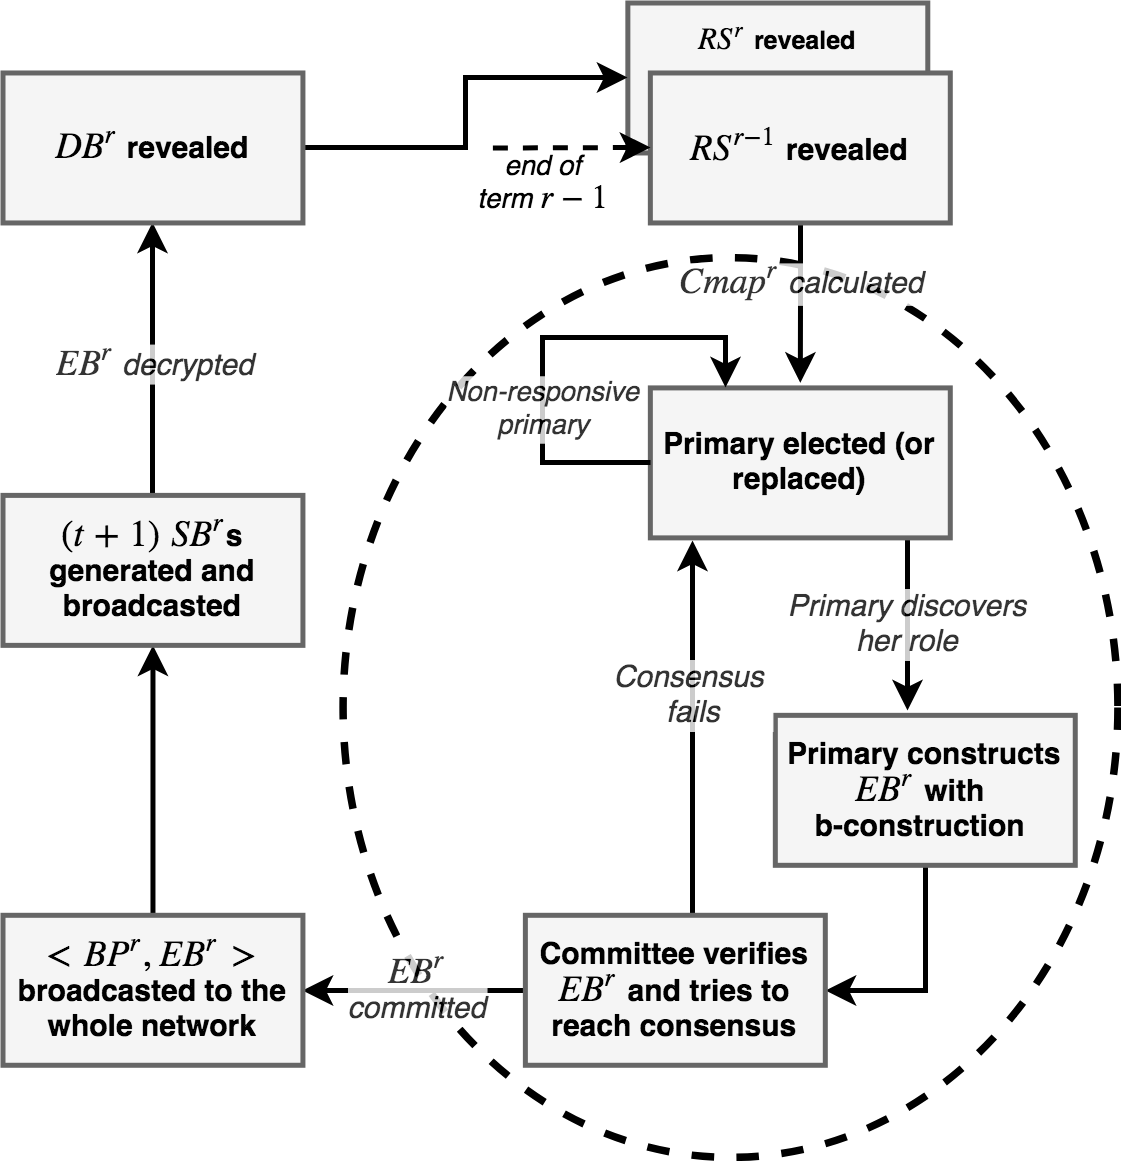
\includegraphics[width=8cm]{Helix_flow.png}
\caption{A high-level, system-view of the dynamics of a \name term. Segment four and the intra-committee communication related to the base agreement protocol lies in the dotted ellipse.}
\label{term_flow}
\end{figure}

\subsubsection*{Segment 1---Initial setup}
Since Helix relies on a threshold cryptosystem, an initial interactive step for key generation is required. A distributed key generation (DKG) protocol among the nodes would be used (e.g.,~\cite{Shoup-Gennaro, Boldyreva, NoLeaderThersholdDK2001}).

\underline{Threshold encryption}. 
We use the DKG to generate a common public key ($PK$), secret keys $(S_0,...,S_{n-1})$ and verification keys $(V_0,...,V_{n-1})$. The $PK$ is known to all entities in the system and is used to encrypt transactions. The secret and verification keys are kept privately by the nodes and are used to decrypt $etx$s. In this article we assume static membership of nodes\footnote{An interesting topic for future investigation is removing the need to redo the setup process every time a node joins or leaves. A possible approach is to generate extra key pairs and distribute them among the nodes according to some secret sharing scheme. When a new node joins she collects enough shares to construct her key pair, in the spirit of~\cite{NoLeaderThersholdDK2001}. Supporting removal of nodes can be more tricky.}.

\underline{Random seed}. 
In every term, a random seed is generated as part of the decryption of the committed Eblock. The initial random seed $RS^0$  is hard-coded into the genesis block. The initial seed will be used to determine the first Cmap and in particular the first committee.
Instead of using a dealer, a (Public)-VSS Coin Tossing scheme can be used to generate $RS^0$~\cite{SCRAP}.

\subsubsection*{Segment 2---$\pmb{etx}$ propagation}
Transactions are issued by users; each user signs and then encrypts each transaction that he issues\footnote{The choice to have users sign and then encrypt transactions favors user's anonymity, but exposes the network to spam attacks. Under our model assumptions, these attacks are mitigated by the nodes, where each node is responsible for her users. As a matter of fact, the bare minimum required is a mechanism that reveals the owner nodes of committed transactions. If this cannot be achieved in a real deployment system, user anonymity can be given up.}. Each user’s unique $sk$ is used for signing, whereas the common $PK$ is used for encryption. The $sk$ is generated locally by each user, whereas the $PK$ is hard-coded into the genesis block\footnote{To address cases in which the $PK$ changes due to a reconfiguration of the participating nodes, it is necessary to have a safe means for updating the users. We leave this discussion for future work.}. After signing and encrypting is complete, the user sends the $etx$ to his owner node.

\underline{Communicating Encrypted-transactions}.
As described previously, each $etx$ is sent by the issuing user to his owner node. The owner node then forwards the $etx$ to all the nodes in the network. A key objective of the forwarding scheme is to reduce the ability of other nodes to identify the original sender node (a node should only certify which $etx$s she owns but will not publicize this until after the Eblock containing her $etx$ is committed). This is crucial for maintaining fairness (as described in Sec.~\ref{section_properties_fairness}). Each node maintains her own Epool by adding new $etx$s she receives and by removing committed $etx$s (i.e., $etx$s included in committed Eblocks). We emphasize that the progress of segment 2 is independent of the advancement of the blockchain as described in segments 3 and 4. 

%user process
\begin{algorithm}
\caption*{\textbf{Process User}}\label{Process:User}
\begin{algorithmic}[1]
	\small
    
    \Statex \text{\fontshape{ui}\selectfont Let $sk$ be the user's secret key and $PK$ the network's }
     \Statex \text{\fontshape{ui}\selectfont public key.}
	%\State \text{\textbf{Input:} Secret key $sk$, public key $PK$ } \textit{// Issuing transaction and sending it}
    \Statex   
	\Indent
    	\Statex \textit{// Issuing transaction and casting it}
		\State $tx \gets \text{IssueNewTransaction}\big(\big) $
		\State $\sigma \gets \text{SignTransaction}\big(tx, sk\big) $  
		\State $etx \gets \text{EncryptTransaction}\big(\langle tx \rangle _{\sigma}, PK\big) $
		\State \text{Unicast\big($etx$\big)} \Comment{to owner node}

	\EndIndent

\end{algorithmic}
\end{algorithm}

\subsubsection*{Segment 3---Spreading consensus}
\label{segment3}
The main purpose of this segment is to update all non-committee members as to the consensus result from the previous term and to kick-start the next one.    

\underline{Eblocks and Block-proofs}.
In a certain term $r$, once the consensus procedure for $EB^r$ has concluded and some committee member has built a valid $BP^r$, the pair $\langle EB^r, BP^r \rangle$ should be propagated to the whole network as rapidly as possible. Once a non-committee member receives the pair $\langle EB^r, BP^r \rangle$, she performs a \emph{brief-validation} and appends $EB^r$ to her blockchain. A brief-validation of a pair $\langle EB^r, BP^r \rangle$ includes the following checks: 
\begin{enumerate}
\item The Cmap appearing in $EB^r$'s header matches the one calculated locally by the node. In particular, a correct node would refuse to append $\langle EB^r, BP^r \rangle$ unless she had already appended the previous Eblock and can calculate the current Cmap and the current committee's composition.  As a matter of fact, this step can be dropped as we explain in Sec.~\ref{section_syncs}.
\item $BP^r$ serves as a valid proof that the base agreement protocol has been carried out successfully (as described in segment four) by the rightful committee (i.e., all signers appearing in $BP^r$ appear in Cmap$^r[0,\dots,m-1]$). 
\end{enumerate}

%Since the correct committee members should have already heard of the current Eblock and independently constructed (or are in the process of constructing) the corresponding $BP$ (as explained in sec.~\ref{layer4}), it makes more sense to first propagate them to the non-committee members. This corresponds to the instructions of the communication protocol in this case.

\underline{Shares-blocks and decryption}.
As briefly noted above, Shares-blocks are constructed by nodes that have committed an Eblock and have not yet received $t+1$ Shares-blocks for that Eblock (this condition is set to reduce the number of Shares-blocks propagating in the network). Normally, committee members would be first to hear of new committed Eblocks and would thus be the ones producing Shares-blocks (this however strongly depends on message propagation in the network). After a node assembles a Shares-block, she broadcasts the Shares-block to all nodes through the fast forwarding scheme. Once a node obtains $t+1$ Shares-blocks for a committed Eblock, the Eblock is decrypted and the Dblock is revealed. We note that from the nature of the threshold encryption scheme, any valid $t+1$ Shares-blocks would produce the same Dblock. The choice $t=f$ minimizes the time from committing an Eblock to decrypting it, while maintaining \nameNS's resilience to $f$ Byzantine (and cooperating) nodes.

% Node process
\begin{algorithm} [htbp] \caption{\label{proc} \textsc{ProcessNode }} 
	\caption*{\textbf{Process Node} (for node $i$)}\label{Process:Node}
	\begin{algorithmic}[1]
    
    	\small

    	% Node's state
        \Statex \text{\fontshape{ui}\selectfont Let $r$ be the term number and $Cmap^r$ the Cmap of term $r$.}
		%\State \text{\textbf{State:} Term $r$, Cmap $Cmap^r$,}      
        
        \Statex    
        % Wait and Decrypt
        \State \text{Upon receiving a briefly validated $\langle EB^r$, $BP^r \rangle$ and $t+1$ $SB^r$s} 
            \Indent
            	
                \State \text{$DB^r \gets $DecryptEblock\big($EB^r$, $SB^r[0,\dots ,t]$\big)}
                \State \text{AppendToBlockchain\big(\big[\footnotesize $EB^r$, $SB^r[0,\dots ,t]$, $BP^r$,$DB^r$\big]\big)}
                \State \text{$Cmap^{r+1} \gets $UpdateCmap\big($DB^r$, $Cmap^{r}$\big)}
                \State $r \gets r+1$
                \State Broadcast$\big( \langle EB^r$, $BP^r\rangle \big)$
                \State \text{If $i \in Cmap^r[0,\dots ,m-1]$}
        		\Indent
                	\State \text{Trigger Process PBFT}
				\EndIndent
            \EndIndent       
	\end{algorithmic}
\end{algorithm}


\subsubsection*{Segment 4---Base agreement protocol}
\label{segment4}
Generally speaking, the base agreement protocol is a single-value variant of PBFT, re-instantiated every term, and responsible for intra-committee consensus regarding the current term's Eblock. The ellipse in Fig.~\ref{term_flow} illustrates segment four within the \name protocol. PBFT, as a Byzantine agreement protocol, enables \name to reach finality, i.e., no two correct nodes ever commit different Eblocks in the same term, as long as the bound $f$ on the number of Byzantine nodes holds (see proof in Sec.~\ref{section_properties_safety}). To emphasize this, \name inherits PBFT's robust safety guarantees---safety is kept even during times the communication network is asynchronous or unreliable. We split the segment's description into two parts. First, we describe segment four as an \emph{ideal agreement protocol} that achieves certain properties. Then, we explain how PBFT is used to implement it.  

\underline{Ideal agreement protocol}. 
The ideal agreement protocol run between $m$ nodes $u_{0},\dots,u_{m-1}$ shall implement the following primitive.
\begin{definition}[ideal agreement protocol]\label{Protocol:BBP}
An agreement protocol is said to implement the ideal agreement protocol for \nameNS's segment four if it satisfies the following properties:
\begin{itemize}
\item Validity. If a correct node commits a value $\alpha$ then some node proposed $\alpha$.
\item Liveness. If all correct nodes initiated the protocol then all correct nodes commit a value.
\item Safety. If a correct node commits a value $\alpha$ then every correct node commits $\alpha$.
\item Verifiability. If a correct node commits a value $\alpha$, then she can produce a proof $p_{\alpha}$, such that anyone can efficiently verify that $\alpha$ was agreed upon by the $m$ nodes.
\end{itemize}
\end{definition}
A typical Byzantine agreement (BA) protocol satisfies the first three items. Nodes that have not participated actively in the BA and wish to commit the agreed-upon value after the fact can do so (safely and efficiently) using the verifiability proof. 
%Verifiability allows anyone to certify the output was indeed agreed by the m participating nodes thus it implies acquaintance, i.e., the verifier must know the participating node prior the verification.realized
\nameNS's base agreement protocol implements the ideal agreement protocol, where $EB^r$ is the value agreed upon and $BP^r$ serves as a proof that it was indeed agreed upon by nodes $u_0,\dots,u_{m-1}$. The question remains though---which nodes are the rightful committee members in term $r$? In order to avoid forks (i.e., inconsistencies), \name must figure out a way for all the participating nodes to come to an agreement as to a single committee. This is done using $EB^{r-1}$ which contains a commitment to the seed that determines the $r$-term committee. Using an inductive argument, if there are no forks in term $r-1$, then only a single committee is possible in term $r$ and accordingly there can neither be forks in term $r$. Finally, since the first committee is hard-coded into the genesis block and agreed upon by all nodes, \name enjoys no forks. 

\underline{Simplified PBFT as the ideal agreement protocol}.
In \nameNS, the ideal agreement protocol is implemented using a simplified version of PBFT~\cite{PBFT} that reaches agreement over a single value. We assume a familiarity with PBFT's logic and terminology and describe Helix's adjustments and modifications to PBFT\footnote{To keep our presentation concise, we leave PBFT's original point-to-point communication intact and do not adopt a more bandwidth-economical protocol such as CoSi~\cite{CoSi} as proposed in Byzcoin~\cite{Byzcoin} or Zilliqa~\cite{Zilliqa}. In \nameNS, optimizations to PBFT's bandwidth consumption can be relieved as we assume $m \ll n$, where $m$ is the size of the committee running PBFT.}.

\textit{Accepting an Eblock}. \label{Protocol:ValidateEB}
In PBFT, a node \emph{accepts} a pre-prepare message (and the value she proposes) by broadcasting a corresponding prepare message after validating the following: 
\begin{enumerate}
\item The view in the pre-prepare message matches her internal view number.
\item The pre-prepare message is signed by the rightful primary in that view.
\item She has not accepted a pre-prepare message in the same view containing a different Eblock.
\end{enumerate}

In \nameNS, when accepting $EB^r$, a correct committee member further validates that:
\begin{enumerate}
\item $EB^r$'s header contains Cmap$^r$ as locally computed with $DB^{r-1}$ and $EB^{r-1}$. We emphasize that a correct committee member does not depend on $EB^r$'s header in order to figure out whether she is in the committee or not. This implies that in order to participate in a committee a correct node must obtain $DB^{r-1}$ and $EB^{r-1}$.
%A correct committee member also checks it appears somewhere in the first $m$ places in Cmap$^r$. 
%(for $RS^{r-1}$ which depends on $MDR^{r-1}$, and the new reputations which can be calculated from the old ones (that appear in Cmap$^{r-1}$), the composer of $EB^{r-1}$ and the view in which it was committed locally for the first time. All these are written in the header of $EB^{r-1}$).
\item $EB^r$'s header contains a valid hash pointer to $EB^{r-1}$.
\item $EB^r$'s header contains a valid hash pointer to $DB^{r-1}$.
\item $EB^r$'s header contains a valid hash of concatenated $ese$s, i.e., $H(ese^r_{i_0},\dots,ese^r_{i_{t}})$, properly signed by the different nodes $i_0,\dots,i_{t}$ (taken from the $t+1$ $SB^{r-1}$s the composer node used in order to decrypt $EB^{r-1}$).
\item $EB^r$'s header contains the correct composer and view (this can be validated with the new-view messages, if exist).
\item $EB^r$'s payload contains at most $b$ $etx$s.
\end{enumerate}

\textit{View-change mechanism}. 
In PBFT, when timeouts expire (e.g., due to a faulty primary or an unexpected network slowdown) view-change messages are broadcasted with the aim of replacing the primary. In order to ensure safety is maintained cross-views, proofs of previously committed values are submitted within the view-change mechanism. To avoid rerunning all the committed values from the beginning of time, a checkpoint mechanism is introduced where proofs are sent only for values that were committed after the last stable checkpoint. 
\nameNS's blockchain construction enables invoking a new instance of a single-value PBFT for each term (this single-value PBFT implements the ideal agreement protocol). Thus, the checkpoint and truncating mechanism can be given up altogether (while primaries keep being replaced seamlessly). In addition, new-view messages contain only one pre-prepare message which never contains the null digest, $d^{null}$. Only in case a new Eblock is proposed, the Eblock itself is passed as regularly done with pre-prepare messages.

\textit{Verifying consensus}.
The verifiability property of the ideal agreement protocol (see definition~\ref{Protocol:BBP}) is obtained by the Block-proof that stores a signed pre-prepare message, $2f$ corresponding signed prepare messages and $2f+1$ corresponding signed commit messages\footnote{We note that in order to reduce the size of such a proof, aggregation of signatures or a threshold signature scheme may be deployed, as in~\cite{Hot-Stuff}.}. On its own, a Block-proof is not enough as a node needs to know the composition of the term's committee and make sure all the signers are indeed committee members. As mentioned before, this can be deduced from the previous term's block. We show in Sec.~\ref{section_properties_safety} that $BP^r$ indeed serves as an unforgeable proof a $EB^r$ was committed-locally by some correct committee member in term $r$. Thus, the pair $\langle EB^r, BP^r \rangle$ (after validation) is safe to append to one's blockchain.

\textit{Timeout mechanism}.
We consider two timeout mechanisms for \nameNS. In PBFT's original approach, timeouts are deterministic and double every time the view increases, i.e., the timer in view $v$ is set to be $2^{v-1} x$, for some positive value $x$. This ensures that in a timely network, all backups will eventually converge to a specific view (that of the current most advanced backup or one view later), even if the network performs unreliably for a restricted amount of time. This technique, although it works in theory, is very problematic (see ~\cite{Prime}) as timeouts must keep growing and cannot be adjusted to be shorter\footnote{As a matter of fact, once a backup commits-locally a value in PBFT, she could potentially start over with timer set to $x$ in the next view, leaving in previous views at most $f$ backups. These would eventually be synced with the checkpoint mechanism.}.

We suggest a different possible timeout mechanism, in which timeouts remain constant and thus highly relies on the network being reliable and predictable in latency. Every time an instance of PBFT is initiated, or when a view-change message is sent, a node's timer is reset to the same value, $x = \max \left\{ 2\Delta, \text{ } \Delta+3\delta \right\}$. In a nutshell, this value is set so that it expires only after a committee member is certain a correct primary had enough time to get her Eblock committed. In the next section, we prove formally that \name is indeed live under the condition any piece of information a node broadcasts (according to the fast forwarding scheme) is received by all correct nodes within a known bound $\Delta$ (see App.~\ref{appendix_comm} that discusses \nameNS's communication schemes).    

%AVI: add highest view value in the NEW-VIEW message....
%Process PBFT
\begin{algorithm*}
	\caption*{\textbf{Process PBFT} (for committee member $i$)}\label{Process:PBFT}
	\begin{algorithmic}[1]  
    	%\algsetup{linenosize=\tiny}
    	\small
        
        
    	\Statex \text{\fontshape{ui}\selectfont Let $r$ be the term's number, Cmap$^r$ the Cmap of term $r$, $v \in \mathbb{N}$ the view, and $CEB$ a candidate Eblock.}
        \Statex \text{\fontshape{ui}\selectfont Let $j \in $Cmap$^r [\,0,\dots,m-1]\,$ be a committee member and $p_v=$Cmap$^r[\,v~mod~m]\,$ be v's primary.}
		%\State  \text{This process is triggered by DecryptProcess.} 
        %\State $\textbf{Input: } \text{Term $r$, Cmap $Cmap^r$. } $
        \Indent
        %\State \textbf{Def: }\text{Let $j \in Cmap^r [\,1,\dots,m]\,$ be a committee member and $p \in Cmap^r[\,1]\,$ be the primary.}
        
       \Statex
		%\Procedure{BackupProcess$\left(Cmap^r,\text{ } r \right)$ }{}
        \Statex \textbf{Init: } \text{$v \gets 0$, $CEB \gets null$, $prepared \gets false$, $committed\_locally \gets false$, $\mathcal{P}_i^r \gets null$.}
        \Statex \textbf{Timer: } \text{Set timer to $x_0=x$ and start countdown.}
        
        \Statex
        
        \Statex \textit{// First primary}
        \State \text{If $i=p_0$,} 
            \Indent
                \State $CEB \gets \text{ConstructEblockFromEpool\big(\big)}$
                \State \text{Multicast$_{committee}$\big($\big\langle\langle \text{PRE-PREPARE, $0$, $r$, H}(CEB)\rangle _{\sigma_{p_0}} \text{, }CEB \big\rangle$\big)}
            \EndIndent
        
        \Statex
        	\Statex \textit{// Normal flow}
            \State $\text{Upon receiving a } \big\langle\langle \text{PRE-PREPARE, $v$, $r$, H}(EB)\rangle _{\sigma_{p_v}} \text{, }EB \big\rangle \text{ message}$
            
            \Indent
                \State \text{ValidateEblock$\big(EB \big)$}  \Comment see Sec.\ref{Protocol:ValidateEB}
                \State $CEB \gets EB$ 
                \State \text{Multicast$_{committee}$\big($\langle \text{PREPARE, $v$, $r$, H}(CEB) \text{, }pk_i\rangle _{\sigma_i}$\big)} 
            \EndIndent

            \State $\text{Upon receiving $2f$ }  \langle \text{PREPARE, $v$, $r$, H}(CEB) \text{, }pk_i\rangle _{\sigma_j} \text{ messages and } CEB \neq null   $ \label{PBFT:Backup:Primary_Join}
            \Indent
                \State $prepared \gets true$
                \State \text{Multicast$_{committee}$\big($\langle \text{COMMIT, $v$, $r$, H}(CEB) \text{, }pk_i\rangle _{\sigma_i}$\big)} 
            \EndIndent

             \State $\text{Upon receiving $2f+1$ } \langle \text{COMMIT, $v$, $r$, H}(CEB) \text{, }pk_i\rangle _{\sigma_j} \text{ messages and } prepared = true$
            \Indent
                \State $committed\_locally \gets true$
				\State $BP \gets \text{ConstructBP\big(\big)}$
                \State \text{PropagateEB\big($  CEB$, $BP$\big)}
            \EndIndent
            
            \Statex 
            \Statex \textit{// Timeout: primary change proposal}
            
            
            
            \State \text{Upon timer expiry, reset timer to $x_{v+1}=2^{v+1} x_0$}
            \Indent
            	\State \text{$\mathcal{P}_i^r = null$}
            	\State \text{If $prepared=true$ then,}
                \Indent
                	\State \text{$\mathcal{P}_i^r = \begin{cases}
       \mathcal{P}_i^r.EB \gets CEB\\
       \mathcal{P}_i^r.msgs_v \gets 2f+1\text{ PREPARE messages with view $v$, received for $CEB$}\\
     \end{cases}$}
                \EndIndent
                \State \text{Unicast$_{p_{v+1}}$\big($\langle \text{VIEW-CHANGE, $v+1$, $r$, $\mathcal{P}_i^r$, } pk_i\rangle _{\sigma_i} $}\big) 
                \State $v \gets v+1$
            \EndIndent
            
            \Statex 
            \Statex \textit{// Primary change takeover, for $p_{\tilde{v}}$}
            
            \State \text{Upon receiving $2f+1$} $\langle \text{VIEW-CHANGE, $\widetilde{v}$, $r$, $\mathcal{P}_j^r$, } pk_j\rangle _{\sigma_j} $ \text{messages, denote them by $\mathcal{V}$}
            \Indent
            	%\State \text{$\mathcal{V} \gets 2f+1$ view-change messages received}
            	\State \text{If there exists a $j$ s.t. $\mathcal{P}_j^r \neq null$ then, } 
                \Indent
                	\State \text{$j \gets$ the node with the maximal $v$ among $\mathcal{P}_j^r.msgs_v$}
                	\State \text{$CEB \gets \mathcal{P}_j^r.EB$}
                \EndIndent
                \State \text{Otherwise,}
                \Indent
                	\State \text{$CEB \gets$ ConstructEblockFromEpool\big(\big)}
                \EndIndent
                \State \text{$\mathcal{O} \gets \big\langle\langle \text{PRE-PREPARE, $\widetilde{v}$, $r$, }H(CEB)\rangle _{\sigma_i} \text{, }CEB \big\rangle$}
                \State \text{Multicast$_{committee}$\big($\langle \text{NEW-VIEW, $\widetilde{v}$, $r$, $\mathcal{V}$, $\mathcal{O}$}\rangle $\big)} \Comment{NEW-VIEW messages, after validated, are treated as} \par
                \Comment{PRE-PREPARE messages by recipients}
            \EndIndent

        \EndIndent     
	\end{algorithmic}
\end{algorithm*}

%\red{Note (terminology): a committed Eblock is an Eblock that was committed locally by at least one correct node and thus has a valid block-proof. It is also guaranteed to be the next Eblock appended to the blockchain.}


%add the partial synchrony timeout scheme and explain why necessary.
%Some terms may be very quick while others might take longer.

\subsection{Incentive mechanism in \nameNS}
\label{Reputation} 
%\red{Looks good. I would just make some changes in the presentation: I think we should start with the fact we want to incentive some behaviors, then present fees (explaining they are paid by nodes to nodes) and reputation (explaining again their influence). We can then give the list of examples, and then refer to the calculation of their inputs.}
Processing a transaction in \name costs money as it consumes resources such as bandwidth, storage and computation. Each node is responsible for the processing costs of transactions issued by her own users\footnote{The way a node covers the costs of her users depends on her business model, e.g., funding may come from the users themselves or from a third party.}. However, the cost for processing transactions for other nodes’ users may be considerable, and thus requires in-protocol compensation from those nodes. If all nodes produce the same amount of transactions, compensation is settled trivially as costs balance. Though if nodes produce different amounts of transactions, a fee mechanism that offsets costs among nodes is required. Fees would basically be paid by nodes with a high transaction rate to those with a low transaction rate\footnote{At this point we do not elaborate as to the implementation of \nameNS's fee mechanism, but assume that the fee is proportional to a node's transaction rate.}. 

Fees, in addition to balancing costs, serve as means to incentivize nodes to follow the protocol's instructions and allow the protocol to reach optimal performance. This is achieved by a reputation score that is attributed to each node and is updated frequently. The reputation strives to serve as a reliable measure to a node's quality of service. A node’s reputation is taken into account when calculating her fee tariffs, where nodes with low reputation can charge lower fees for their services than their peers, possibly resulting in losses. For this reason, it is important that both the measurement of the resource usage and of the quality of service are accurate. %(or: resources and behavior)

%Gruffalo's fee mechanism is based on a trusted third party\footnote{This entity can be represented by a smart contract\red{, in a different platform or over Gruffalo itself}.} that collects fees from nodes and pays them back later taking into account their issuance rate and reputation. In practice the third party would transfer funds from nodes with high usage to those with low usage taking into account nodes' reputation. Nodes with low reputation will be paid back less than their relative share, resulting in losses. Thus, it is crucial that Gruffalo's fee mechanism will measure accurately the usage of each node and that the reputation will measure correctly nodes' resources and behavior.

Measuring a node's usage is straightforward after revealing the owner nodes of all $etx$s in the decryption process. Making sure the reputation is consistent with \nameNS's requirements and instructions is more complicated. We suggest a few practical criteria that the reputation may examine, but a more elaborate discussion as to its exact specification is due at a later time. We further note that with the evolution of the system, the reputation measure may be enhanced to mitigate new found vulnerabilities in the protocol or to encourage new desired behaviors. The discussion above makes clear that nodes are incentivized to increase their reputation, but also wish to include their own $etx$s in Eblocks as fast as possible. These two distinct preferences may be conflicting, requiring nodes to prioritize.

We shall now illustrate a naive reputation measure. It is updated frequently (e.g., every 1000 blocks or every month), locally and deterministically by each node, according to the blockchain. A few concrete examples:
\begin{itemize}
\item In order to make sure that nodes maintain high uptime and stay available, every node is evaluated according to the average view number of committed Eblocks when she was a committee member. The higher the average view, the lower the reputation should be.
\item In order to make sure that nodes maintain the recent blockchain history, if an Eblock consists of a previously included $etx$, its composer should be punished by reducing hers reputation.
\item In order to make sure that nodes select $etx$s randomly (see Sec.~\ref{section_highload} for more details), adjacent Eblocks should represent similar distributions (in terms of the owner nodes of the $etx$s they include). If a specific node is found to construct Eblocks that significantly deviate from the Eblocks in their surrounding, she should be penalized by reducing her reputation.
\item In order to encourage nodes to stay up-to-date with protocol changes, a node that constructs an Eblock with a decommissioned protocol version should be penalized by reducing her reputation.
\end{itemize}

We emphasize that the reputation update rules that do not depend on Dblocks may be used as validation checks in the agreement protocol. On the contrary, some of the validation checks in Sec.~\ref{Protocol:ValidateEB} may be relaxed and become a part of the reputation mechanism. %These two mechanisms share a common goal---to have the blockchain represent nodes' needs and desires. 
An interesting possibility is to relate reputation to a node's stake in the system. We also note that the reputation measure is shared across other services in the system such as the execution service.




\section{Basic properties and proofs}
\label{section_properties}
\name achieves three desired properties: safety, liveness and fairness. First and foremost, \name is \emph{safe}. As long as the bound $f$ on the number of Byzantine (rather than sleepy) nodes holds, even without any assumptions on network synchrony, forks cannot happen (i.e., there will not be a situation in which different nodes commit different blocks in the same term).
Second, \name is \emph{live}. We refer to two types of liveness. First, under a weakly synchronous network \name achieves (eventual) liveness, meaning that new blocks are (eventually) added to the blockchain in some finite time. Second, we show that under a strongly synchronous network \name achieves a stronger property referred to as \emph{strong liveness}, in which new blocks are added within a known bounded period of time.
Finally, \name is \emph{fair} with regard to three types of fairness. The first two refer to fairness among nodes: election fairness (of committee members) and selection fairness (of transactions in Eblocks). The third type refers to fairness towards users. In this section, we elaborate on each of these three properties and prove that the \name protocol fulfills them. %We rely on the notations and assumptions defined in the previous sections.  
%Question: Is it true that safety depends on Cmap being explicitly written in the Eblock? This is especially interesting under the fast sync optimization. Could we generate a fork if nodes only compute Cmap locally and make sure all the signatures in the Block-proof belong to the committee they calculated locally. In the fast sync not having the committee in the Eblock introduces new difficulties as nodes that do not belong to the committee might sign and non-synced nodes cannot verify this as they have no idea what the committee is and it is not written in the Eblock...... 
\subsection{Safety}
\label{section_properties_safety}
\name is designed to provide safety even in the case of a slow and unreliable communication network. Safety implies finality, meaning that once an Eblock has been appended to the blockchain in the eyes of any (even one) correct node, then no correct node ever appends a different Eblock for that term. The safety of \name relies on the safety of its underlying protocol, PBFT~\cite{PBFT}.  

\begin{claim}{(\name is safe)}
Let $0,\dots,n-1$ be the nodes running \nameNS. In term $r$, let $EB^r_i$ and $EB^r_j$ be Eblocks appended by correct nodes $i,j\in [n-1]$, respectively, to their local blockchains. Then, $EB^r_i=EB^r_j$.
\end{claim}
\begin{proof}
For PBFT's proof to be applicable here, we need to show that the committee in term $r$ is a well-defined and agreed-upon set of $m$ nodes. Put differently, we need to show that no correct node can be ``tricked'' into believing she is a committee member when she is actually not, submitting signatures for invalid Eblocks. This is easily prevented by relying on the previous term's Eblock (or more accurately Dblock) to determine the next term's committee. A simple inductive argument can convince that there can be only a single version of $DB^{r-1}$ and thus the composition of the $r$-term committee is well defined. Since all nodes compute the $r$-term committee from their $r$-term Dblock, all correct nodes will agree as to its composition. This concludes the proof using PBFT's safety proof. 
\end{proof}
%old proof - formal induction, too long, too complicated.
% We prove the claim by induction on $r$. We split the proof into three sections. 
% %We assume that $r$ is not the first term. The proof for the case in which $r$ is the first term is similar, relying on the genesis block which is shared between all the nodes before the protocol starts.  

% \begin{itemize}
% \item Agreement on committee members: We first show that the committee of term $r$, denoted $C^r$, is a well-defined set of $m$ nodes, i.e., that all correct nodes running \name either agree on $C^r$ or have not yet discovered it. From the induction hypothesis all correct nodes that appended an Eblock in term $r-1$ appended the same Eblock. We denote this Eblock by $EB^{r-1}$. From \nameNS's decryption mechanism and Cmap calculation, we deduce that all correct nodes that appended and decrypted $EB^{r-1}$ hold the same Cmap in term $r$, denoted Cmap$^r$. $C^r$ is simply the first $m$ nodes in Cmap$^r$. The rest of the correct nodes have not yet calculated a Cmap in term $r$.  

% \item Agreement on Block-proofs: From safety in PBFT, we show that any two valid $r$-term Block-proofs correspond to the same $r$-term Eblock (we emphasize that valid Block-proofs in the same term may differ). From our model assumptions there can be at most $f$ Byzantine nodes among the $m=3f+1$ members in $C^r$\footnote{We note that there can be correct nodes in $C^r$ that are not aware of being committee members and thus do not participate and are considered sleepy. In an asynchronous network a sleepy node cannot be distinguished from a slow one and thus is not taken into the $f$ count.}. If a Block-proof exists (it might be the case that a third party intercepted the messages and constructed a Block-proof locally before any of the committee members does so) for a given Eblock, $EB^r$,
% %\footnote{A Block-proof consists of a pre-prepare message proposing $EB^r$, $2f$ corresponding prepare messages and $2f+1$  corresponding commit messages, all containing a matching $\langle view, term, H(EB^r) \rangle$ and signed by nodes in $C^r$.}
% then $EB^r$ could have been committed-locally by some node in term $r$. From PBFT's safety, $EB^r$ is the only block that can be committed-locally in term $r$ and thus, any other valid set of such messages could solely relate to the same Eblock.

% \item Agreement on the Eblock corresponding to a given term: Last, we show that $EB^r_i=EB^r_j$ for any correct nodes $u_i$ and $u_j$. In \name there are exactly two ways to append an Eblock in term $r$. The first is to participate in a committee and commit-locally an Eblock that has undergone all the $r$-term PBFT phases. The second is to receive a valid pair $\langle EB^r, BP^r \rangle$ from another node in the network. In both cases, an Eblock is appended only once a valid Block-proof is obtained. That means $EB^r_i$ comes with $BP^r_i$ and $EB^r_j$ comes with $BP^r_j$. From the previous item we know that they relate to the same Eblock, concluding $EB^r_i=EB^r_j$.   
% %If both $u_i$ and $u_j$ have committed-locally their respective Eblocks, $EB^r_i$ and $EB^r_j$, then, from PBFT's safety, $EB^r_i= EB^r_j$. Otherwise, if, w.l.o.g. only $u_i$ committed-locally $EB^r_i$, and has constructed a valid Block-proof for its Eblock $BP^r_i$ (this notation relates to the first version of $BP^r$ that node $i$ adopted, either constructing it locally or receiving it from another node), then by the previous item it follows that $BP^r_i$ and $BP^r_j$ relate to the same Eblock, implying that $EB^r_i= EB^r_j$. Finally, if neither $u_i$ nor $u_j$ committed their Eblocks locally, but instead received $\langle EB^r_i, BP^r_i \rangle$ and $\langle EB^r_j, BP^r_j \rangle$, respectively, then again, by the previous item, the Block-proofs $BP^r_i$ and $BP^r_j$ relate to the same Eblock. In all cases, $EB^r_i=EB^r_j$.
% \end{itemize}
%\end{proof}

\subsection{Liveness}
\label{section_properties_liveness}
In its most general sense, liveness guarantees that new blocks are added to the blockchain in some finite time. We consider two types of liveness which correspond to different synchrony assumptions and timeout mechanisms. 

\subsubsection*{General liveness}
For \name to be live in the general sense, we need each PBFT instance to be live and for each member of the subsequent committee to (eventually) realize that she has been assigned to this role. For this to hold, we need the same synchrony assumptions as in PBFT, namely, a weakly synchronous network, where message delay is arbitrary up to a certain point but is eventually bounded by some unknown bound. 
\begin{claim}{(\name is live)} 
Among $n$ nodes, \name (with the doubling timeout mechanism) continues to make progress, meaning that regardless of the internal state of the nodes, within some finite time, some correct node will commit a new Eblock to her blockchain.
\end{claim}
\begin{proof}
The proof follows from  PBFT's liveness and the fact that committee members eventually become aware of their committee membership. Assume that the last Eblock to be committed by a correct node was in term $r-1$. We identify three possible system states:
\begin{itemize}
\item State 1: At least $2f+1$ correct nodes are aware of their participation in term $r$'s PBFT instance concurrently. In this case, by the liveness property in PBFT, in a finite time, at least one of them will append a valid Eblock to her blockchain.
\item State 2: Fewer than $2f+1$ correct committee members are aware of their committee membership, but at least one correct node knows the identities of the committee members for term $r$. This node has the ability (and duty, so to speak) to update all the committee members for term $r$ (safety guarantees that this will not contradict any other correct node's view of term $r$'s committee members) by sending them $EB^r$, $BP^r$ and $t+1$ $SB^r$s. A simple syncing and feedback protocol\footnote{We do not get into the details of this protocol, but it is clear that as long as messages are eventually delivered, this information will propagate.} 
%Ronen: maybe add a reference if possible, this is a little vague maybe? See for example section 4.2 in Tendermint paper for example of how they handle the issue} 
run between the nodes ensures that this information is eventually propagated to all correct nodes. Accordingly, after a finite period of time state 1 takes place.
\item State 3: No correct node is aware of the composition of term $r$'s committee. According to the protocol, the correct node that appended $(r-1)$'s Eblock to her blockchain is in the process of decrypting it (again, safety guarantees no forks in the  term $r-1$). The decryption process duration depends only on the time of message dispersal, i.e., propagation of the committed Eblock, its Block-proof and $t+1$ Shares-blocks. Thus, the process of decrypting term $(r-1)$'s Eblock is finite. Once at least one correct node decrypts the committed Eblock, we are back in state 2, which concludes the proof. \qedhere
\end{itemize}
\end{proof}


\subsubsection*{Strong liveness}
In \nameNS, we wish to obtain a stronger notion of liveness that relies on two additional requirements. First, we require a time frame in which new blocks are committed. Second, we aim for a correct primary to succeed in committing her Eblock before a new primary is appointed. The first of these requirements is driven by the need for practical liveness (with a guaranteed bound on progress time), whereas the second requirement is related to fairness (discussed in Sec.~\ref{section_properties_fairness}). We refer to this stricter notion of liveness as \emph{strong liveness}. For strong liveness to hold in \name we require the network to be strongly synchronous, namely, message delay is assumed to be bounded by some known constant (as explained in detail in Sec.~\ref{section_model}). To obtain strong liveness in \name we use the constant timeout mechanism, in which $x = \max\left\{ 2\Delta, \text{ } \Delta+3\delta \right\}$ is set as the timeout, as mentioned in Sec.~\ref{segment4}. %Ronen: $\delta$ and $\Delta$ are functions of node bandwidth, network latency, and other factors, so while they allow us to prove a theoretic claim, in practice I don't see how one could find the appropriate setting for the timeouts using them. In that case, I'm not sure I see the reason to prove this property.

\begin{definition}{(Strong liveness)}
\label{definition_strong_liveness}
A blockchain protocol (that enjoys finality), run between $n$ participants is said to be strongly live if it satisfies the following properties:
\begin{enumerate}
\item A primary that proposes a valid block, immediately after its construction, gets it committed.
\item A correct node that appended the $(r-1)$-term block, appends the $r$-term block within some known bounded period of time.
\end{enumerate}
\end{definition}

Before proceeding, recall the network model assumptions: $\Delta$ is the maximal time it takes for a message that a correct node broadcasts, according to the fast forwarding scheme, to reach all correct nodes; and $\delta$ is the maximal time it takes for point-to-point messages to arrive at their destinations. The relationship between $\delta$ and $\Delta$ depends on the communication protocol\footnote{In general gossip communication, where nodes send a new piece of information to some random group of neighbor nodes, a bound like $\Delta$ usually refers to the time it takes to reach a certain percentage of the network, say $90\%$. This is because the last nodes are hard to reach in such probabilistic protocols as was shown specifically for the Bitcoin network in~\cite{BitcoinPropagation}.} as discussed in Sec.~\ref{section_model}.

We now prove that \name (with the constant timeout mechanism) is strongly live if the network is strongly synchronous. We distinguish between two cases based on the status of the first primary. First, we denote by $u_r$ the first correct node to reveal $DB^r$ at time $\tau_r$, and with it, Cmap$^{r+1}$.
\begin{lemma}{(Term with a correct first primary)}
If the first primary Cmap$^r[0]$ is correct, she will get $EB^r$ committed prior to any correct member’s timeout expiring.
\end{lemma}
\begin{proof}
In term $r$, $u_{r-1}$'s initial timeout will be the first among the correct nodes to expire (at time $\tau_{r-1}+x$). Since $u_{r-1}$ follows the communication protocol, she has propagated each piece of information she has heard or produced so far (in particular $EB^{r-1}$, $BP^{r-1}$ and some $t+1$ $SB^{r-1}$s) and thus necessarily  all nodes reveal $DB^{r-1}$ (and Cmap$^r$) by time $\tau_{r-1}+\Delta$. In particular, the first committee's primary (since assumed to be correct) would realize her role by time $\tau_{r-1}+\Delta$ and would multicast a pre-prepared message with $EB^r$ to all committee members of term $r$. This message would reach all correct committee members by time $\tau_{r-1}+\Delta+\delta$ (intra-committee communication is done point-to-point).
%Ronen: This implicitly assumes the leader can simultaneously unicast a block to each committee member, for large block sizes this isn't the case. 
Then, by time $\tau_{r-1}+\Delta+2 \delta$ all correct committee members should receive enough prepare messages and by time $\tau_{r-1}+\Delta+3 \delta$, $EB^r$ should be committed-locally by all correct committee members. Since all correct nodes' timers expire later than $\tau_{r-1}+\Delta+3 \delta$, no timeouts expire before $EB^r$ is committed-locally by all as required.
\end{proof}

\begin{lemma}{(Term with a faulty first primary)}
Assume Cmap$^r[0]$,$\dots$,Cmap$^r[i-1]$ are all faulty nodes and Cmap$^r[i]$ is a correct node, where $i \in \{ 1, \dots ,f \}$. Then, $EB^r$ will be committed-locally by all correct committee members in a view $v \in \{ 1, \dots ,i \}$.
\end{lemma}
\begin{proof}
If $EB^r$ is committed-locally, by even a single correct member, in view $j<i$, we are done because a correct committed-locally member would propagate $\langle EB^r, BP^r\rangle$ to all correct nodes within $\Delta$ time. This ensures that any correct committee member would append $EB^r$ to her blockchain prior to sending a view-change message for the $(j+2)^\text{th}$ time (i.e., within its $j+1$ view). The $(j+2)^\text{th}$ view-change message can be sent, the earliest at $\tau_{r-1}+(j+2)x$, on the other hand, $\langle EB^r, BP^r\rangle$ would reach all nodes, the latest at $\tau_{r-1}+(j+1)x+2\Delta$. Indeed, we have $x\geq 2\Delta$.

Otherwise, we show that all correct members commit-locally $EB^r$ in view $i$. Denote the first correct committee member to send Cmap$^r[i]$ a view-change message by $u$. The earliest time $u$ can send this message is $\tau_{r-1}^i=\tau_{r-1}+i \cdot x$. Since no other correct node had already committed-locally, all correct nodes keep sending view-change messages every $x$ time. Thus, if two correct members enter term $r$ in some time difference, then they keep sending view-change messages with the same time difference. As was shown in the first case, this difference is bounded by $\Delta$. Thus, by $\tau_{r-1}^i+\Delta$ all correct nodes would send Cmap$^r[i]$ a view-change message and Cmap$^r[i]$, being correct, would reply with a new-view message containing a valid Eblock $EB^r$, that would reach all correct committee members by time $\tau_{r-1}^i+\Delta+\delta$. As was explained before, by $\tau_{r-1}^i+\Delta+3\delta$, $EB^r$ would be committed-locally by all correct committee members. Since all the $(i+1)^\text{th}$ timers expire later than $\tau_{r-1}^i+\Delta+3\delta$, none should expire before committing-locally $EB^r$ as required.
\end{proof}

\begin{corollary}{(\name is strongly live)}
If \name is run over a strong synchronous network (with the constant timeout mechanism), it is strongly live.
\end{corollary}
\begin{proof}
The first property (in definition~\ref{definition_strong_liveness}) is deduced directly from the two previous lemmas.

To conclude the second property in the definition, we look at a correct node that appended $EB^{r-1}$. Since the network is strongly synchronous, then from the fast forwarding scheme, $EB^{r-1}$ would propagate to all correct nodes within $\Delta$ time and decrypted within another $\Delta$ time. Once $DB^{r-1}$ is revealed, the two lemmas above become relevant---the more view-changes, the longer it takes to reach agreement as to the $r$-term Eblock. Since there could be at most $f$ faulty nodes within the term-$r$ committee, we saw that there can be at most $f$ view-changes after which it is certain a correct primary is appointed. A correct primary gets her Eblock committed in another $3\delta$ time. Since every view lasts exactly $x$ time, we conclude that a node that appended $EB^{r-1}$ would append $EB^r$ in (at most) $2\Delta+f\cdot x+3\delta$ time.
\end{proof}
We note that if \name is run with the doubling timeout mechanism, nonetheless \name is strongly live, only with a longer bound. 

\subsection{Fairness}
\label{section_properties_fairness}
\name achieves \emph{fairness} in three aspects. \emph{Election fairness} relates to the amount of terms in which a node participates as committee member. Fairness in this sense implies that a node's participation level is proportional to her resource holdings, which in our system is related to reputation\footnote{In PoW systems, the resource is proportional to the computational ability to solve partial hash-collision puzzles. In PoS systems, the resource is proportional to stake in the system. In \nameNS, reputation is a concept that reflects how aligned a node is with the protocol's instructions.}. \emph{Fairness towards users} relates to mechanisms that limit nodes' capabilities in discriminating or censoring users' transactions. In this section we discuss election fairness and fairness towards users in Helix. In the following section we analyze the third type of fairness, \emph{selection fairness}, which thrives to achieve a blockchain in which the representation of nodes (according to their $etx$s) is proportional to their \emph{transaction rate}.


\subsubsection*{Election fairness}
\label{section_voting_fairness}
In blockchain protocols, nodes (sometimes referred to as miners) compete in a lottery to find blocks, where a node can increase her probability of winning, if she has more \emph{resources}. We consider this lottery as \emph{fair} if a node's probability of winning a block (or being given the right to propose a block) is proportional to her holdings in the resource. We denote node $i$'s resource holdings in term $r$ as $res^r_i$ and her proportionate share as $rep^r_i = \frac{res^r_i}{\sum_j res^r_j}$.

\begin{definition}{(Election fairness)}
A blockchain protocol, where nodes are randomly elected to propose blocks according to a resource holdings $rep$, is said to be \emph{election-fair} if the probability of node $i$ to be elected as the composer of the block in term $r$ is $rep^r_i$.
\end{definition}

Nakamoto consensus for example is not election-fair---selfish mining attacks are possible by a strong adversary with $p_a \geq 0.25$, increasing her probability to find a block over $p_a$ as was shown in \cite{SelfishMining, SelfishMiningStrategies}. Another example is Algorand~\cite{AlgorandV9}, which falls a bit short---there, a leader knows before the network what the next random seed would be in case her block is accepted. Thus, she can choose between two options---either to propose a block or not to. This introduces an advantage to the leader, even if small. The main goal in this section is to prove the following claim:

\begin{claim}{(Election fairness)} \label{claim:ele_fair}
\name is election-fair with respect to reputation as the resource, assuming at most $f$ nodes are Byzantine (i.e., deviate from the protocol).
\end{claim}

We note that in the context of \nameNS, election fairness is more relevant to consider in terms of committee membership rather than leader election. 
We proceed to prove claim~\ref{claim:ele_fair} with the following argument: since Cmap$^r$ is determined by $RS^r$, it is enough to show that $RS^r$ serves as a randomness beacon. That is, the adversary (or any other node) cannot manipulate or foresee $RS^r$ prior to its ``global" disclosure. Put formally,
\begin{lemma}
A set of nodes running \name can use $RS^r$ as a common and unpredictable string of bits. Specifically, for every $r$:
\begin{enumerate}
\item Two correct nodes $i$ and $j$ with $RS^r_i$ and $RS^r_j$ have $RS^r_i=RS^r_j$.
\item Prior to $EB^r$ being committed by at least one correct node, none of the bits in $RS^r$ can be predicted with probability greater than $1/2$ by the adversary (with non-negligible probability). 
\end{enumerate}  
\end{lemma}

\noindent Before the proof, we recall the fact that a valid Eblock must contain exactly $t+1$ signed (and distinct) $ese$s (see Sec.~\ref{Protocol:ValidateEB}).
\begin{proof}
$ $\\
\begin{enumerate}
\item The first item follows directly from Helix's safety.
\item Regarding the second item, consider the adversary that wishes to predict $RS^r$ given a candidate valid $EB^r$ (considering a non-valid Eblock is irrelevant as it would never be committed) that has not yet been committed by even a single correct node. $EB^r$ must contain exactly $t+1$ distinct $ese$s and the adversary needs to predict $RS^r=se^r_0 \oplus \dots \oplus se^r_{t}$. We show that none of the bits in $RS^r$ can be predicted with probability grater than $1/2$. Pick an arbitrary bit in $RS^r$, $z=z_0 \oplus \dots \oplus z_{t}$ where $z_i$ is the corresponding bit in $se^r_i$.
Before $EB^r$ being committed, the adversary has access to $ese^r_0,\dots,ese^r_{t}$. From the assumption that at most $f<t+1$ nodes are controlled by the adversary, and from the security of the encryption scheme, the adversary knows at most $t$ $z_i$s (the adversary knows the $(t+1)$th $z_i$ with negligible probability). Without loss of generality, be these bits $z_0,\dots,z_{t-1}$. This implies that $z_t$ is sampled by an honest node, i.e., in the eyes of the adversary $z_t$ can be modeled as an unbiased Bernoulli random variable.
Additionally, the encryption scheme used by \name is non-malleable~\cite{malleable}, which means the adversary cannot correlate her $ese$s to $ese_t$ such that the corresponding $se$s are related. This implies that (again, from the eyes of the adversary) $z_t$ is sampled independently from any other $z_i$ for $0\leq i \leq t-1$. To conclude, the adversary can denote $z=w\oplus z_t$, where $w$ is known and $z_t$ is an unbiased Bernoulli random variable sampled independently from $w$. It is a well-known fact that due to the XOR operation $z$ can also be regarded as an unbiased Bernoulli random variable, which completes the proof.  \qedhere
\end{enumerate}
\end{proof}

\noindent We are now ready to prove claim~\ref{claim:ele_fair}.
\begin{proof}
Recall that node $i$'s value in Cmap$^r$ is defined as follows: $$v_i^{r+1}:=\frac{H(RS^r,r+1,pk_i)}{rep^{r+1}_i}$$ and that the $m$ nodes with the minimal values are the committee members in term $r+1$. Since $RS^r$ serves as a non-manipulable source of randomness, we conclude that the values $\big\{H(RS^r,r+1,pk_i)\big\}_{i=0}^{n-1}$ induce a random ordering of the nodes, and the values $\{ v_i^{r+1} \}_{i=0}^{n-1}$, induce a random ordering weighted by reputation.   
\end{proof}
We draw the reader's attention to a nice benefit of the random seed in \nameNS, namely that $RS^r$ is independent of $RS^{r-1}$. This is rather surprising as $RS^r$ is constructed iteratively (or rather, we are exposed to its values iteratively).


\subsubsection*{Fairness towards users}
This section describes the problem of fairness towards users in high-level and illustrates \nameNS's approach. 
In general, nodes and users are very different entities in blockchain protocols. Users are the entities issuing the transactions but they cannot directly append them to the blockchain. Users depend on their nodes for \emph{write} operations. Nodes proposing blocks can use this power in malicious ways---they can order transactions in a block according to their will, censor certain transactions, etc. 

The key factor in reducing nodes' ability to manipulate the blockchain is $etx$ indistinguishability. Ideally, two $etx$s propagated through the network are indistinguishable---in terms of their issuer nodes, sizes, or any other criteria (of course, a node knows which $etx$s she issued). Thereby, using a suitable encryption scheme that hides transaction information is necessary\footnote{Note that such indistinguishability facilitates spam attacks. To mitigate this problem, we intend on using a scheme that allows a subset of the nodes to trace the issuer of any $etx$ in question. Such a scheme can be realized via group signatures with distributed traceability~\cite{SignaturesWithDistributedTraceability,SignaturesWithThresholdTraceability}.}. This is realized in \name using two mechanisms:
\begin{itemize}
\item A threshold encryption scheme that takes place on the user end, concealing the actual content of transactions from nodes. The content is revealed only after the inclusion of the transaction in a block is finalized and its location in the blockchain can no longer be altered.
\item $etx$s are forwarded in \name in a manner that maximizes the sender's anonymity such that nodes are not aware who is the owner node of a transaction they receive.
\end{itemize}

We further illustrate how reducing nodes' information regarding transactions plays a role in \nameNS's resilience to a few common attacks against users:
\begin{itemize}
\item Payment censorship. In this attack, any transaction aimed to ``pay'' a certain user is denied and not processed. This attack is impossible in \name as the nodes have no clue who is the payee in an $etx$\footnote{During this article we tried to disregard any semantics attributed to transactions, this item is exceptional in that sense and assumes transactions have two sides---payers and payees.}. 

\item Service censorship. In this attack, any transaction issued by a certain user is denied service and never added to the blockchain. In case an owner node can identify an $etx$ issuer, she can refuse to propagate it or add it to Eblocks she proposes. This problem can be mitigated quite simply by allowing users to have multiple owner nodes, forwarding $etx$s to all of them\footnote{An alternative solution is to have another dedicated service: a transaction-forwarding service. For the time being \name handles both---the forwarding and the ordering services. Although this might change in the future as means to align subtle issues with the incentive structure and the mentioned attack.}.

\item Ordering manipulation. In this attack, later transactions are processed before earlier ones. This can be considered an attack only if the system should be \emph{order-fair} in some sense. Bitcoin for example is not order-fair in any sense, and as a matter of fact, this is considered one of Bitcoin's strengths---a high-priority later transaction can ``bypass'' earlier low-priority transactions by offering a higher fee. In a distributed system as \nameNS, the seemingly simple notion of \emph{$tx_1$ is earlier then $tx_2$} (denoted $tx_1<tx_2$) is not easy to define. A proper example of such a definition is given in Hashgraph \cite{Hashgraph}. Hashgraph is shown to be order-fair in the sense that the ledger's order reflects the order by which transactions reached a certain fraction of the entire network. \name is not fair in this sense, but suggests another concept of fairness in terms of ordering transactions. Intuitively, if an entity orders transactions she cannot relate any semantics to, there is nothing she can do other then ordering them randomly. In this spirit, we refer to an ordering of two transactions $tx_1$ and $tx_2$ as fair, if at the time of ordering, the ordering entity could not have determined which order is more \emph{profitable} for her.
\name is order-fair in this sense when the more profitable order---$tx_1<tx_2$ or $tx_2<tx_1$, depends on the content of both $tx_1$ and $tx_2$. Assuming at least one of these transactions was issued by a user, the ordering node is familiar only with the corresponding $etx$ and cannot extract any useful information from it. Thus, in this scenario, we conclude that the order of transactions \name produces is fair. The best example to illustrate Helix's resilience to order manipulation in this regard is front-running\footnote{Front-running is a form of market manipulation practice where an entity with non-public information exploits it to produce an unfair profit. Consider the following example, a user sends a transaction with an order to buy a large amount of shares of some stock. Since the buy order will drive the price of the stock up, the node receiving the transaction can push her own buy transaction beforehand, where she can buy the stock's shares before the price rises. Later, the node releases the user's transaction and sells her recently bought shares at a higher price.}.
In the next section we show that Helix is also fair in regards to another ordering manipulation where nodes service $etx$s owned by them prior to other nodes' $etx$s. This ordering manipulation does not depend on the content of transactions, but only on the ability to classify a transaction as owned by a specific node. It is crucial (and non-trivial) for Helix to be resilient to such manipulations under the incentive structure Helix assumes. We refer to this as \emph{selection fairness}.
\end{itemize}


\section{Selection fairness via correlated sampling}
\label{section_highload}
%motivation - representation fairness
Thus far we discussed \nameNS's mechanisms for combating transaction censorship and ensuring fair primary (and committee) election. We now turn to the more subtle procedure of constructing blocks from the pool of pending transactions.

In typical blockchain protocols, nodes (such as Bitcoin's miners) have the freedom to select which transactions to include in their blocks. Normally, when transactions come along with a fee determined by the issuer, this results in a fee market that drives fees unnecessarily high at times of high demand. While we do not elaborate on \nameNS's fee structure, we emphasize that \name is designed such that fees do not play a role in $etx$ selection\footnote{This design choice enables a variety of fee mechanisms e.g., constant fee per transaction, periodic subscription fees, and models in which fees are determined after processing.}. This design choice makes sense when fees are not needed as the main motivation of nodes to include transactions in blocks. Indeed, our presumption in \name is that nodes have inherent interest in processing their own transactions\footnote{For instance, nodes run consumer applications and wish to service their end-users by processing the transactions they issue.}. 
Under these circumstances, the main goal of this section is to describe \nameNS's mechanism for selecting $etx$s in a \emph{fair} manner. Fairness in this regard should be reflected by the blockchain, representing each node according to the proportion of $etx$s she owns\footnote{Under such notion of fairness nodes may be encouraged to artificially produce many self-owned transactions in order to get more block real-estate. Carefully designed fee mechanisms could disincentive such behavior, e.g., paying increased fee for failing transactions.}.

An important aspect in the context of fair sampling is the relation between the rate at which $etx$s are issued and the rate at which they are appended to the blockchain. An epoch at which the \emph{issuance rate} is smaller than the maximal \emph{append rate} (allowed by the system) is relatively easy to analyze---all transactions are processed within a small time frame. A more involved case is when the issuance rate is (temporarily) greater than the append rate. During such epochs, there are many $etx$s pending to be added to the blockchain, and the decision of which $etx$s to include in Eblocks is subject to manipulation. The core aspect of selection fairness is to ensure that the average \emph{waiting time} of an $etx$ depends solely on the number of pending transactions, rather than on its owner node or on any other characteristic.   

In high-load epochs, we adapt a strategy of \emph{correlated sampling} that restricts the freedom a primary has in selecting which $etx$s to include in her Eblock.
%way $etx$s are selected to be included in Eblocks. 
Correlated sampling, considered in~\cite{HashSample1,HashSample2,HashSample3} (see also~\cite{OptCorSampling} for a review and optimality result), refers to the problem in which there are two players having different distributions over the same domain (in our case the set of issued $etx$s) and access to shared randomness (in our case the random seed). Each player wishes to output a single element, sampled according to her distribution while minimizing the probability that the outputs differ. In the work of~\cite{HashSample1}, a MinHash strategy was used for performing correlated sampling for the case that the distributions are uniform over a subset of the domain (analogous to Epools in our setting). In~\cite{hashsamplemultiple}, Rivest applied the MinHash strategy sequentially in order to sample many elements from the domain, possibly with repetitions. However, to the best of our knowledge the scenario of correlated sampling of many elements without repetitions has not been analyzed before.   

%Section structure
Instead of dictating an Eblock construction strategy that might not be aligned with primaries' selfish interests and might be difficult to validate, we suggest an Eblock validation procedure that is better aligned with nodes' interests. In the following section we describe the Eblock validation procedure applied in \name in accordance with the correlated sampling scheme. We then show that strategies with substantial probability of passing validation remain close to the construction dictated by the correlated sampling scheme. Throughout this section we restrict ourselves to high-load epochs by assuming that the total number of pending $etx$s is $\Gamma b$ for some $\Gamma > 1$ (where $b$ is the maximal number of $etx$s in a valid Eblock). 

\subsection{Eblock validation} \label{Validation}
%common ordering of $etx$s in Epool in term $r$.
The \name correlated sampling scheme uses a hash function in order to serialize candidate $etx$s for the next Eblock. The hash function is tweaked with a random seed to eliminate its predictability, yielding a common, random and unpredictable serialization of the $etx$s. Formally, when considering the Eblock in term $r$, the nodes order the pending $etx$s according to the values $H(RS^{r-1},etx)$, and refer to these values as the \textit{hash values} of the $etx$s. We denote $H(etx)$ for brevity. 

%where the dot to the left of $H$ denotes the binary fraction the hash represents, so all hash values are in $[0,1]$. We assume the hash function distributes these values uniformly in $[0,1]$, and conclude that the probability of an $etx$ to be hashed below a given threshold $T\in [0,1]$ is exactly $T$. For brevity we usually write $H(etx)$ rather than $.H(RS^{r-1},etx)$. 

%Introducing locking times
To ensure unpredictability, we introduce the notion of \textit{locking time}. We denote by $EP_i^\tau$ node $i$'s locked Epool at time $\tau$, which is a snapshot of the $etx$s in $i$'s Epool at time $\tau$\footnote{This can be implemented by attaching a timestamp to each $etx$ at the time it was received.}. We denote by $\tau_i'$ the time at which node $i$ revealed $DB^{r-1}$, and define the locking time of node $i$ to be $\tau_i:=\tau_i'-2\Delta$ (recall the definition of $\Delta$ from Sec.~\ref{communication_schemes} as the upper bound on the dissemination time between any pair of nodes).

%upshot of locking times
In the validation procedure, nodes are asked to consider the serialized $etx$s in their Epool at locking time. The choice of $\tau_i$ was made such that nodes cannot quickly tailor $etx$s with low hash values \emph{after} revealing the random seed, but \emph{before} the rest of the network does.  Indeed, due to network latency it could be the case that $RS^{r-1}$ is revealed to some node before the rest of the network---by at most $2\Delta$ time. Without the notion of locking time nodes could have exploited this time to generate and forward tailored $etx$s, detracting from the randomness of the common ordering. Restricting nodes to consider only $etx$s which were known to them prior to time $\tau_i'-2\Delta$ prevents this kind of attack. From now on by writing $EP_i$ we mean $EP_i^{\tau_i}$, unless stated otherwise.

%A primary is asked to include in its Eblock the $b$-minimal hashed $etx$s of its Epool (\textit{$b$-minimal Eblock construction}). Each committee member is asked to validate this selection by comparing the primary's Eblock with the set of lowest hashed $etx$s in its own Epool. The primary's Eblock is validated iff for enough committee members, the intersection of these two sets is large enough.

%The validation conditions are set such that even though different Epools differ slightly due to network latency, correct nodes accept the $b$-minimal construction with overwhelming probability. If, on the other hand, the primary chooses to include in its Eblock $etx$s which are not among its $b$ minimal $etx$s, then this Eblock has a lower probability of passing validation and is more likely to get rejected. 

%Notations and notions we use in the validation procedure

Due to network latency and inherent properties of \nameNS, we cannot expect $EP_i$ and $EP_j$ to be identical, even if $i$ and $j$ are correct nodes. However, as locking times are similar, we may assume a measure of similarity between two correct Epools at locking times.
%\footnote{Entities with ability to predict network timing may conduct an attack that results in correct Epools being largely dissimilar. To mitigate such an attack, $\tau_i$ can be modified to $\tau_i:=\tau_i'-2\Delta-\eta_i$, where $\eta_i$ is locally sampled by $i$ in the range $[0,\Delta]$. This would decouple the predictability of the network from the locking-time procedure.}. 
To model this similarity, we use a probabilistic model satisfying the following property. For any two correct nodes $i,j$ each $etx$ in $EP_i$ is in $EP_j$ with probability at least $\alpha$. We refer to $\alpha$ as the \emph{similarity parameter} of the network.
%\footnote{Notice that this model clearly ignores the fact that an $etx$ which was issued by node $i$ is certainly in $EP_i$. We ignore this fact strictly for brevity.}.

%\red{To model this we consider the set $GP$, which is the \emph{global Epool} of round $r$, defined as $GP = \cup_{i}EP_i^{t_i}$ where the union is done over all correct nodes $i$. The Epools similarity can now be modeled precisely by a simple probabilistic model. $EP_i$ is a random sample of $GP$, containing any $etx$ from $GP$ with probability at least $\alpha$.}

Upon receiving a proposed Eblock, $EB_p$, from primary $p$, correct committee member $i$ validates it by performing the validation procedure presented in Sec.~\ref{Protocol:ValidateEB}. In addition, she checks two conditions regarding the size of the proposed Eblock and the size of its overlap with a set of transactions calculated according to her own Epool. 
We define $T_p$ be the maximal hash of an $etx$ in $EB_p$, i.e., $T_p:=\max\{H(etx)\vert etx\in EB_p\}$. Likewise, we denote by $EB_i' :=\{etx\in EP_i|H(etx)\leq T_p\}$ the set of $etx$s in $EP_i$ with hash values lower than $T_p$, and $b_i:=\max\{|EB_i'|,b\}$. We further denote by $b'$ the size of $EB_p'=\{etx\in EP_p|H(etx)\leq T_p\}$ and say that $EB_p$ was constructed under a $b'$-construction. 
This illustrates the fact that $EB_p$ was selected as a subset of size $b$ among the $b'$ lowest hashed $etx$s in $EP_p$ such that the $b'^{\text{th}}$ $etx$ was included. The setting is illustrated in Fig.~\ref{fig_correlated_sampling}.


\begin{figure}
%[!b]%[!ht]
	\centering
\begin{tikzpicture}
\tikzstyle{every loop}=[]
\draw (0,0) rectangle (1.8,2.5);
\draw (2.8,0) rectangle (4.6,6);
\draw (7.2,0) rectangle (9,6);

\filldraw[black] (0.1,-0.25) circle (0pt) node[anchor=west] {Proposed};
\filldraw[black] (0.3,-0.6) circle (0pt) node[anchor=west] {Eblock};
\filldraw[black] (0,-0.95) circle (0pt) node[anchor=west] {(of $b$ $etx$s)};
\filldraw[black] (3.00,-0.25) circle (0pt) node[anchor=west] {Primary $p$};
\filldraw[black] (2.60,-0.6) circle (0pt) node[anchor=west] {(following the};
\filldraw[black] (2.60,-0.95) circle (0pt) node[anchor=west] {$b'$-construction)};
\filldraw[black] (7.45,-0.25) circle (0pt) node[anchor=west] {Correct};
\filldraw[black] (7.25,-0.6) circle (0pt) node[anchor=west] {committee};
\filldraw[black] (7.30,-0.95) circle (0pt) node[anchor=west] {member $i$};


\filldraw[black] (0.35,2.75) circle (0pt) node[anchor=west] {$EB_p$};
\filldraw[black] (3.25,6.25) circle (0pt) node[anchor=west] {$EP_p$};
\filldraw[black] (7.65,6.25) circle (0pt) node[anchor=west] {$EP_i$};

\filldraw[black] (0.4,0.35) circle (0pt) node[anchor=west] {$etx_{1}$};
\filldraw[black] (0.4,0.7) circle (0pt) node[anchor=west] {$etx_{3}$};
\filldraw[black] (0.4,1.4) circle (0pt) node[anchor=west] {$etx_{j}$};
\filldraw[black] (0.4,2.15) circle (0pt) node[anchor=west] {$etx_{b'}$};
%\filldraw[black] (0.5,5.65) circle (0pt) node[anchor=west] {$etx_{|EP_P|}$};

\filldraw[black] (3.2,0.35) circle (0pt) node[anchor=west] {$\boldsymbol{etx_{1}}$};
\filldraw[black] (3.2,0.7) circle (0pt) node[anchor=west] {$etx_{2}$};
\filldraw[black] (3.2,1.05) circle (0pt) node[anchor=west] {$\boldsymbol{etx_{3}}$};
\filldraw[black] (3.2,1.9) circle (0pt) node[anchor=west] {$etx_{j-1}$};
\filldraw[black] (3.2,2.25) circle (0pt) node[anchor=west] {$\boldsymbol{etx_{j}}$};
\filldraw[black] (3.2,3.15) circle (0pt) node[anchor=west] {$\boldsymbol{etx_{b'}}$};
\filldraw[black] (3.2,3.85) circle (0pt) node[anchor=west] {$etx_{b'+1}$};
\filldraw[black] (3.1,5.65) circle (0pt) node[anchor=west] {$etx_{|EP_P|}$};

\draw [decorate,decoration={brace,amplitude=10pt,mirror},xshift=4pt,yshift=0pt]
(4.5,0) -- (4.5,3.5) node [black,midway,xshift=0.6cm, yshift=0.2cm] 
{\footnotesize $EB'_p$};

\filldraw[black] (7.6,0.35) circle (0pt) node[anchor=west] {$etx'_{1}$};
\filldraw[black] (7.6,0.75) circle (0pt) node[anchor=west] {$etx'_{2}$};
\filldraw[black] (7.6,1.15) circle (0pt) node[anchor=west] {$etx'_{3}$};
\filldraw[black] (7.6,3.15) circle (0pt) node[anchor=west] {$etx'_{b_i}$};
\filldraw[black] (7.6,3.85) circle (0pt) node[anchor=west] {$etx'_{b_i+1}$};
\filldraw[black] (7.6,5.65) circle (0pt) node[anchor=west] {$etx'_{|EP_i|}$};

\draw [decorate,decoration={brace,amplitude=10pt},xshift=4pt,yshift=0pt]
(7.0,0) -- (7.0,3.5) node [black,midway,xshift=-0.6cm, yshift=-0.3cm] 
{\footnotesize $EB'_i$};

\filldraw[black] (4.7,3.8) circle (0pt) node[anchor=west] {$T_p = H(etx_{b'})$};
\draw [-,dashed,thick, blue, line width=0.75mm] (2.8,3.5) to  (9,3.5);

\draw [->,dashed,thick, red, line width=0.75mm] (3.2,0.35) to (1.3,0.35);  
\draw [->,dashed,thick, red, line width=0.75mm] (3.2,1.125) to (1.3,0.7);  
\draw [->,dashed,thick, red, line width=0.75mm] (3.2,2.25) to (1.3,1.4);  
\draw [->,dashed,thick, red, line width=0.75mm] (3.2,3.155) to (1.3,2.25); 



 \path[]
 ;
\end{tikzpicture}
 \caption{Illustration of the correlated sampling validation process. In each Epool, $etx$s are sorted based on their hash values. A threshold $T_p$ is determined by the maximal hash value of an $etx$ in the EBlock $EB_p$ proposed by the primary $p$. A correct committee member $i$ examines the overlap between $EB_p$ and the set of $etx$s in $EP_i$ which hash below $T_p$.	}\label{fig_correlated_sampling}
\end{figure}






% \begin{figure}
% %[!b]%[!ht]
% 	\centering
% \begin{tikzpicture}
% \tikzstyle{every loop}=[]
% \draw (0,0) rectangle (1.8,2.5);
% \draw (2.8,0) rectangle (4.6,6);
% \draw (7.2,0) rectangle (9,6);

% \filldraw[black] (0.1,-0.25) circle (0pt) node[anchor=west] {Proposed};
% \filldraw[black] (0.3,-0.55) circle (0pt) node[anchor=west] {block};
% \filldraw[black] (0,-0.85) circle (0pt) node[anchor=west] {(of $b$ $etx$s)};
% \filldraw[black] (3.00,-0.25) circle (0pt) node[anchor=west] {Leader $l$};
% \filldraw[black] (7.20,-0.25) circle (0pt) node[anchor=west] {Verifier};
% %\filldraw[black] (7.30,-0.55) circle (0pt) node[anchor=west] {member $i$};


% \filldraw[black] (0.5,2.75) circle (0pt) node[anchor=west] {$B_l$};
% \filldraw[black] (3.5,6.25) circle (0pt) node[anchor=west] {$P_l$};
% \filldraw[black] (7.5,6.25) circle (0pt) node[anchor=west] {$P_i$};

% \filldraw[black] (0.4,0.35) circle (0pt) node[anchor=west] {$etx_{1}$};
% \filldraw[black] (0.4,0.7) circle (0pt) node[anchor=west] {$etx_{2}$};
% \filldraw[black] (0.4,1.4) circle (0pt) node[anchor=west] {$etx_{j}$};
% \filldraw[black] (0.4,2.15) circle (0pt) node[anchor=west] {$etx_{b}$};
% %\filldraw[black] (0.5,5.65) circle (0pt) node[anchor=west] {$etx_{|EP_P|}$};

% \filldraw[black] (3.2,0.35) circle (0pt) node[anchor=west] {$\boldsymbol{etx_{1}}$};
% \filldraw[black] (3.2,0.7) circle (0pt) node[anchor=west] {$\boldsymbol{etx_{2}}$};
% \filldraw[black] (3.2,1.05) circle (0pt) node[anchor=west] {$\boldsymbol{etx_{3}}$};
% \filldraw[black] (3.2,1.9) circle (0pt) node[anchor=west] {$\boldsymbol{etx_{j-1}}$};
% \filldraw[black] (3.2,2.25) circle (0pt) node[anchor=west] {$\boldsymbol{etx_{b}}$};
% \filldraw[black] (3.2,3.15) circle (0pt) node[anchor=west] {$etx_{b'}$};
% \filldraw[black] (3.2,3.85) circle (0pt) node[anchor=west] {$etx_{b'+1}$};
% \filldraw[black] (3.1,5.65) circle (0pt) node[anchor=west] {$etx_{|P_l|}$};

% \draw [decorate,decoration={brace,amplitude=10pt,mirror},xshift=4pt,yshift=0pt]
% (4.5,0) -- (4.5,2.5) node [black,midway,xshift=0.6cm, yshift=0.2cm] 
% {\footnotesize $B'_l$};

% \filldraw[black] (7.6,0.35) circle (0pt) node[anchor=west] {$etx'_{1}$};
% \filldraw[black] (7.6,0.7) circle (0pt) node[anchor=west] {$etx'_{2}$};
% \filldraw[black] (7.6,1.05) circle (0pt) node[anchor=west] {$etx'_{3}$};
% \filldraw[black] (7.6,3.15) circle (0pt) node[anchor=west] {$etx'_{b_i}$};
% \filldraw[black] (7.6,3.85) circle (0pt) node[anchor=west] {$etx'_{b_i+1}$};
% \filldraw[black] (7.6,5.65) circle (0pt) node[anchor=west] {$etx'_{|P_i|}$};

% \draw [decorate,decoration={brace,amplitude=10pt},xshift=4pt,yshift=0pt]
% (7.0,0) -- (7.0,2.5) node [black,midway,xshift=-0.6cm, yshift=-0.3cm] 
% {\footnotesize $B'_i$};

% \filldraw[black] (4.7,2.8) circle (0pt) node[anchor=west] {$T = H(etx_{b})$};
% \draw [-,dashed,thick, blue, line width=0.75mm] (0,2.5) to  (9,2.5);

% \draw [->,dashed,thick, red, line width=0.75mm] (3.2,0.35) to (1.3,0.35);  
% \draw [->,dashed,thick, red, line width=0.75mm] (3.2,1.125) to (1.3,1.125);  
% \draw [->,dashed,thick, red, line width=0.75mm] (3.2,2.25) to (1.3,2.25);  
%\draw [->,dashed,thick, red, line width=0.75mm] (3.2,3.155) to (1.3,2.25); 



%  \path[]
%  ;
% \end{tikzpicture}
% \end{figure}

Under these notations, the validation checks (in the context of selection fairness) performed by correct node $i$ upon receiving a proposed Eblock, $EB_p$ (from primary $p$), are:
\begin{enumerate}
	\item $|EB_p|=b$ \label{validiation_condition_1}
	\item $|EB_p\cap EB_i'|\geq \beta_{\alpha}(b_i)$ for $\beta_{\alpha}(b_i) :=  \alpha b_i-\sqrt{10 b_i}$ \label{validiation_condition_2}
\end{enumerate}

\noindent The second condition encourages primaries to construct Eblocks with low $b'$. The minimal value of $b'$ is $b$; in the event that the value of $b'$ is in fact $b$, the selection scheme is perfectly fair. Intuitively, a larger $b'$ allows the primary more freedom in the selection of $EB_p$ (rather than selecting it as the $b$ minimal $etx$s). However, since we can expect $|EB_p'| \approx  |EB_i'|$, large $b'$ yields large $b_i$ and accordingly large $\beta_\alpha(b_i)$, reducing the chances of $EB_p$ to pass validation. $\beta_\alpha(b_i)$ is the maximal value for which Eblocks constructed with $b'=b$ pass validation w.o.p., as implied by Hoeffding's bound. This is shown formally in the next section.

% Notice that the larger $|EB_p'\setminus EB_p|=b'-b$ is, the more freedom the primary had in selecting which $etx$s to include in $EB_p$. Since Epools similarity results in $|EB_p'|\sim |EB_i'|$

% $EB_p$ If $EB_p$ is indeed the $b$-minimal $etx$s of $EP_p$, then $EB_p=EB_p'$. It is achieved since on the one hand, $|EB_p\cap EB_i'|$ should be roughly $\alpha b$. Thus, if $b_i\sim b$ then $EB_p$ should pass this validation. On the other hand, $|EB_i'|\sim |EB_p'|$
% when $b'\ge b$ then $T_p'\ge T_i$ and the validation condition becomes $|EB_p'\cap EB_i'|\ge \gamma(b_i)b_i$. Both sides of this inequality grow with $T_p'$, but while the left hand side grows slowly, and is bounded by $b$, the right hand grows faster and is effectively un

% is that if $EB_p$ is composed of the $b$-minimal $etx$s in $EP_p$, then $EB_p=EB_P'$. Since we can expect $EB_p'$ and $EB_i'$ to be quite similar to one another, $EB_p\cap EB_i'$ approximates 

% To formulate the conditions checked in the validation procedure, we introduce the following notions and notations:
% \begin{itemize}
% 	\item $T_p':=max\{H(etx)\vert etx\in EB_p\}$.   \item $EB_p':=\big|\{etx\in EP_p|H(etx)\leq T_p'\}\big|$. We further denote $b':=|EB_p'|$, and note that $EB_p\subset EB_p'$ and is of size $b$. 
% 	\item $EB_i':=\{etx\in EP_i|H(etx)\leq T_p'\}$. We denote $b_i':=|EB_i'|$.
%     \item $EB_i$ is the set of $b$-minimal $etx$s in $EP_i$. 
%     \red{We denote by $T_i$ the maximal hash value of an $etx$s from $EB_i$.}
% \end{itemize}
% We define $b_i:=b_i'=|EB_i'|$ in case $T_i<T_p'$, and $b_i=b=|EB_p|$ otherwise. Notice that in case $T_i<T_p'$, it holds that $EB_i\subset EB_i'$ and $b_i\ge b$.

%intuition for validation conditions 
% We wish to give some intuition regarding the second validation condition. Consider the construction in which the Eblock contains exactly the $b$ $etx$s with lowest hash values in $EP_p$. I.e., this is a $b$-minimal construction. This construction emulates a perfect random construction in terms of the owner nodes representation. Our validation condition is set to check that $EB_p$ does not deviate from this construction by a lot. 
% The way this is done is the following. In the $b$-minimal construction, $T_p'=T_p$, and $EB_p=EB_p'$. In this case, we can expect $b_i'$ to be roughly $b$. Node $i$ should also expect $EP_p$ to contain at least an $\alpha$-fraction of $EB_i'$, which are roughly $\alpha b_i'$. If this is the case,If $EB_p$ was indeed constructed using the $b$-minimal construction then $EB_p\cap EB_i'=EP_p\cap EB_i'$, and so, on average $|EB_p\cap EB_i'|\sim \alpha b_i$ (recall in this case $b_i:=|EB_i'|$). The purpose of the validation condition is to make sure that this more or less the case.

% \textbf{Tradeoff in the selection of $\pmb{\beta}$}: Setting the function $\beta$ is a critical task. On the one hand, a large $\beta(b_i)$ guarantees solid correlated sampling resulting in \emph{representation fairness}, which is simply to say that nodes' representation in each Eblock is similar to their relative part in the overall issued $etx$s. On the other hand, the larger $\beta(b_i)$ is, committee members are more strict in validating Eblocks. Thus, potential differences between Epools of correct nodes might result in Eblocks being rejected often, and guaranteeing liveness becomes more difficult. %\red{further explanation needed, I would rephrase}. 

\subsection{Liveness under $b$-construction} \label{Liveness}
%The problem in Helix terms
The extra validation process dictated by the correlated sampling scheme bears risk to the liveness of the protocol. Blocks that would have passed validation might get rejected once correlated sampling validation is enforced. We thus prove that an Eblock compliant with the $b$-construction passes validation of any correct committee member w.o.p.

\begin{claim} [Liveness under $b$-construction.] \label{liveness} Let $EB_p$ be an Eblock constructed according to the $b$-construction, $i$ be a correct committee member. Then, $EB_p$ passes $i$'s validation w.o.p. (under the assumption that $\alpha$ bounds from below the similarity parameter of the network)
\end{claim}
\noindent We use the following lemma.
\begin{lemma}
For two correct nodes $k,l$ and a general set $A\subset EP_l$, $|A\cap EP_k|>\beta_\alpha(|A|)$ with probability greater then $1-2\exp(-20)$, where $\beta_\alpha(x):=\alpha x-\sqrt{10x}$.
\end{lemma}
\begin{proof}
Denote $Y:=|A\cap EP_k|$. We can write $Y=\sum_{etx\in A}Y_{etx}$, where $Y_{etx}$ are indicator random variables, 
\begin{equation*}
    		Y_{etx} =	
		    \begin{cases}
    			  1  &\mbox{if }  etx\in EP_k \\
     			  0  &\mbox{otherwise}
		     \end{cases}
  	\end{equation*}
By definition, these random variables are i.i.d. Bernoulli variables, with success probability (at least) $\alpha$. This is true from the similarity assumption. By Hoeffding's inequality, for any $\delta \ge 0$
$$Pr \left( \frac{1}{|A|}|Y-\mathbb{E}(Y)| >\delta \right) \leq 2\exp(-2|A|\delta^2)$$
%Bounding the above probability by $2\exp(-20)$, we derive an inequality $2|A|\delta^2 \ge 20\iff \delta \ge \sqrt{\frac{10}{|A|}}$.
The expected value of $Y$ is bounded from below by $\alpha |A|$, thus taking $\delta=\sqrt{\frac{10}{|A|}}$ and plugging this into the left-hand side of Hoeffding's inequality, we get that with probability $>1-2\exp(-20)$ 
\begin{equation*}\begin{split}|A\cap EP_i|= Y&>\mathbb{E}(Y)-|A|\delta\\ &\ge \alpha\cdot |A|-\sqrt{10|A|}=:\beta(|A|) \qedhere
\end{split}\end{equation*} 
\end{proof}

\noindent We now turn to prove claim~\ref{liveness}. 
\begin{proof}
Node $i$'s validation comprises of two checks. Check number~\ref{validiation_condition_1} is that $|EB_p|=b$, which passes with probability $1$. For clarity of the proof, we break check number~\ref{validiation_condition_2} into two:
\begin{enumerate}
	\item[2.1] $|EB_p\cap EB_i'|\geq \beta_{\alpha}(b)$ 
	\item[2.2] $|EB_p\cap EB_i'|\geq \beta_{\alpha}(|EB_i'|)$
\end{enumerate}
For $2.1$, take $A=EB_p\subset EP_p$. For a correct primary, this is simply a general random set of transactions of size $b$. The above lemma can be used as $|EB_p\cap EB_i'|=|EB_p\cap EP_i|$, yielding that the probability for failing this condition is at most $2\exp(-20)$.
The argument for condition $2.2$ is similar, only this time $A=EB_i'\subset EP_i$ and we use the equality $|EB_i'\cap EB_p |=|EB_i'\cap EP_p|$. The latter equality is derived from the assumption that $EB_p$ is a $b$-construction, which implies $EB_p=EB_p'=\{etx\in EP_p|H(etx)\leq T_p\}$. Now, the equality is easily derived from the definition of $EB_i'$.
%Combining the probabilities for $2.1$ and $2.2$ concludes the proof. \red{conditions 2.1 and 2.2 merge into one condition only when $\beta_\alpha(b_i)$ is a monotonically increasing function which is true only when $b_i\geq2.5/\alpha^2$, note that for $\alpha\geq0.5$, $b_i$ should be $\geq10$.}
\end{proof}

 
%Proof of claim (formal)
The claim establishes the fact that a primary following the $b$-construction would pass validation w.o.p., thus keeping the protocol live. 
In the next section we generalize the analysis above, considering Eblocks admitting $b'$-constructions for $b'>b$.




% \begin{tikzpicture} \label{graph11}
%   \begin{axis}[ 
%     xlabel={probability for passing validation ($q$)},
%     ylabel={maximal $etx$ (b'(q))$/1000$},
%     xmin=0.5, xmax=1,
%     ymin=1090, ymax=1120,
%     xtick={0.5,0.6,0.7,0.8,0.9,0.95},
%     ytick={1100,1105,1110,1115,1120}
%   ] 
%   \addplot [
%     color=blue,
%     mark=square,
%     ]
%     coordinates {
%     (0.9377,1100)(0.9053,1102)(0.8693,1104)(0.8371,1106)(0.7833,1108)(0.7231,1110)(0.6578,1112)(0.5979,1114)
%     }
%     \addplot [
%     color=red,
%     mark=square,
%     dashed
%     ]
%     coordinates {
%     (0.986,0.97, 0.948, 0.92, 0.880.8199999999999998
% 0.7199999999999998
% 0.5199999999999995
%     };
%   \end{axis}
% \end{tikzpicture}
% \red{TABLE, GRAPH?}
% Before we continue we note that while the values $\beta(b_i) = \alpha^2b_i-\sqrt{10b_i}$ and $\beta'=\alpha b_i-\sqrt{10b_i}$ are functions of the similarity bound $\alpha$ and the block size $b$, a lower bound on the value of $\beta$ holds in practical settings.
% %b = 200 or 2000 ??
% For $\alpha \ge 0.95$ and $b \ge 2000$ it satisfies $\beta \ge 0.83$. 
% Table~\ref{tab:table1} illustrates the values of $\beta$ for $\alpha \in \{0.90,0.95\}, b \in \{1000,2000,5000\}$. Values of $\beta$ are also presented 
% in Fig.~\ref{fig:beta_vs_alpha}.  
 
% \begin{table}[h!]
%   \begin{center}
%     \caption{$\beta$ calculated for different values of $\alpha$ and $b$}
%     \label{tab:table1}
%     \begin{tabular}{c|c|c|c} % <-- Alignments: 1st column left, 2nd middle and 3rd right, with vertical lines in between
%       $b$ & $\alpha$ &$\alpha ^2$ &  $\beta$ \\
%       \hline
%       1000&0.90 &0.8100&0.7100\\
%       1000&0.95 &0.9025&0.8025\\
%       2000&0.90 & 0.8100 & 0.7393\\
%       2000&0.95 &0.9025&0.8317\\
%       5000&0.90 & 0.8100 & 0.7653\\
%       5000&0.95 &0.9025&0.8578\\
%     \end{tabular}
%   \end{center}
% \end{table}


% \begin{figure}[!t]%[!ht]
% \centering
% \begin{tikzpicture}
% \begin{axis}[
% xmode=log,
%    xlabel={block size $b$},
%    ylabel={$\beta$},
%     %ylabel={$\phi(x)$},
%     xmin=1000, xmax=50000,
%     ymin=0, ymax=1,
%     xtick={1000, 2000, 5000, 10000, 20000,50000},
%     xticklabels={1K, 2K, 5K, 10K, 20K,50K},
%     ytick={0,0.2,0.4,0.6,0.8,1},
%     legend pos=north west,
%     ymajorgrids=true,
%     grid style=dashed,
%     height = 6.2cm,
%     width = 0.50*\textwidth,
%  %   line width=1.6pt,
% %]
%                 legend style={at={(0.65,0.05)},anchor=south west,font=\scriptsize},
%                 label style={font=\footnotesize}, grid=both];
%             %\addplot [black,mark=x] table [x={chi}, y={cooperative}] {\resfirsta};
%         \addplot[% only marks, mark=square,  black,mark=
%    color=red,mark=*,scale=10, line width=1pt,mark options={line width=0.9pt,draw=red,fill=red}]
%     coordinates {
% (1000, 0.8025) (1400, 0.8179845745271483) (2000, 0.8317893218813452) (3000, 0.8447649730810374) (5000, 0.8577786404500042) (7000, 0.8647035526990773)(10000, 0.8708772233983162) (14000, 0.8757738758087575) (20000, 0.8801393202250021) (35000, 0.8855969149054297) (50000, 0.8883578643762691)
%     };
%     \addlegendentry{$\alpha = 0.95$};
%     \addplot[% only marks, mark=square,  black,mark=
%    color=green,mark=triangle,%dotted, 
%    scale=10, line width=1pt,mark options={line width=0.9pt,draw=green,fill=green}]
%     coordinates {
%         (1000, 0.7100000000000001) (1400, 0.7254845745271484) (2000, 0.7392893218813453) (3000, 0.7522649730810375) (5000, 0.7652786404500043) (7000, 0.7722035526990774) (10000, 0.7783772233983163) (14000, 0.7832738758087576) (20000, 0.7876393202250022) (35000, 0.7930969149054298) (50000, 0.7958578643762692)
%     };
%     \addlegendentry{$\alpha = 0.9$};
% \addplot[% only marks, mark=square,
%    color=gray,mark=square,scale=10, line width=1pt,mark options={line width=0.5pt,draw=gray,fill=gray}]
%     coordinates {
%    (1000, 0.5400000000000001) (1400, 0.5554845745271485) (2000, 0.5692893218813454) (3000, 0.5822649730810375) (5000, 0.5952786404500043) (7000, 0.6022035526990774) (10000, 0.6083772233983163) (14000, 0.6132738758087577) (20000, 0.6176393202250022) (35000, 0.6230969149054298) (50000, 0.6258578643762692)
%     };
%     \addlegendentry{$\alpha = 0.8$};
% \end{axis}
% \end{tikzpicture}
% \caption{The value of $\beta$ calculated for different values of $\alpha$ and $b$}
% \label{fig:beta_vs_alpha}
% \end{figure}


\subsection{Selection fairness}\label{subsec:selectionFairness}
%fairness in terms of waiting time.


%In high-load epochs Epools contain many pending $etx$s and primaries have the freedom of choosing which $etx$s to include in new Eblocks they propose. The main motivation behind selection fairness is to restrict this freedom and ensure that the selection process does not favor $etx$ונ יממs of a certain group. Precisely, selectל ion fairness strives to reach a state where the average \emph{waiting time} of an $etx$ depends solely on the לsמטמize of the global Epool, and not on its owner node or on any other characteristic.   

%nodes can manipulate waiting time due to liveness constraints in the validation process.
Under conditions where all nodes follow the $b$-construction, the core aspect of selection fairness is an immediate result---an $etx$ is included in the next Eblock with probability $1/\Gamma$. However, as nodes are assumed to prioritize their own $etx$s and act to shorten their average waiting time, they might choose to follow a different strategy. The inevitable ``room for error'' permitted in the validation process (due to potentially non-identical Epools), prohibits such behavior from being completely eliminated. In this section we analyze the extent to which the validation scheme suggested above can guarantee selection fairness and a fair average waiting time.
%Specifically, we consider two methods that primaries may adopt in order to include more of their $etx$s in Eblocks and show how these influence the average waiting time of their $etx$s. 
%Specifically, we consider two methods that primaries may adopt in order to include more of their $etx$s in Eblocks and show how these influence the average waiting time of their $etx$s.  

%Presenting the two Eblock construction strategies
We consider two distinct methods to manipulate the selection process.
The first is by \emph{tailoring} $etx$s in order to hash them to low values. %Precisely, once the random seed is revealed, the primary tailors prioritized $etx$s such that they  have low hash values, keeping the maximal hash in the Eblock, $T_p$, low. 
The second method is through $b'$-constructions, for $b'>b$. We study the dependency between $b'$ and the certainty of an Eblock to pass validation. %While this analysis may be useful to \name nodes in tuning the parameter $b'$, our main goal is to 
%We deduce analytical, as well as experimental results as to the effect these constructions have on the probability of some $etx$ to get included in $EB_p$.


%Intuition for first strategy - tailoring $etx$s
We start with a high-level analysis of the tailoring approach. While the locking mechanism discussed earlier eliminates the advantage of revealing the random seed prior to the rest of the network, tailoring $etx$s can still be a worthwhile strategy. Issuing many tailored copies of the same transaction and forwarding them to the network would increase the probability of one copy to be processed quickly. In order to avoid such behavior, suitable fee models are needed\footnote{For example, one such fee model can be realized by a system rule that dictates an increased fee for failed transactions. In UtxO-based architectures (like Bitcoin), such an approach would be easier to enforce. In account-based architectures that support rich scripting languages (like Ethereum), circumventing such rules would be considerably impractical.}. 

Alternatively, nodes may keep their tailored $etx$s hidden from the network and include them only when constructing Eblocks. %Note that the probability of a hidden $etx$ to be included in the next Eblock is typically lower than that of a non-tailored $etx$ forwarded to the network. The former probability is $1/n$ (which is the probability of the issuer node to be elected primary), whereas the latter probability is (close to) $1/\Gamma$. A healthy distributed system should not reach a situation where $\Gamma>n$. Additionally, even if a node chooses to hide tailored $etx$s, 
the \name Eblock validation process prevents over-exploiting this strategy. Specifically, since tailored $etx$s are clearly not in $EP_i$, including many of them reduces $|EB_p\cap EB_i'|$, while in order to pass validation, the size of this intersection must be at least $\beta_{\alpha}(b)$.

%Analysis for second strategy - $b'$-minimal.
We continue with a formal analysis of the $b'$-construction. According to this strategy, the primary first looks at $EB_p'$ which contains the lowest $b'$ $etx$s in $EP_p$. Of those, she selects the $b$ $etx$s she prefers. Our analysis ignores this choice and is applicable to any subset of $b$ $etx$s from $EB_p'$ (that includes the $b'^{\text{th}}$ $etx$). Typically, when $b'\ge b$ the validation condition becomes $|EB_p\cap EB_i'|\ge \beta(|EB_i'|)$. Both sides of this inequality grow with $b'$, but while the left-hand side grows slowly, and is bounded by $b$, the right-hand side grows faster and is effectively unbounded. Thus, a large $b'$ decreases the probability of $EB_p$ to pass validation. A quantitative analysis is given hereafter.

%From $b'$ to $T_p'$
We fix some $b'>b$ and consider $EB_p$ constructed via the $b'$-construction. We calculate the probability $q=q(b')$ in which $EB_p$ passes a single validation. Denote this event by $A=A(b')$. 

%$|EB_p\cap EB_i'|$ assumption
Before continuing, we make a simplifying (average-case) assumption. Clearly, $|EB_p\cap EB_i'|$ is bounded from above by $b$, and we will assume that it is exactly $\alpha b$, as the probability of an $etx \in EP_p$ to be in $EP_i$ is (at least) $\alpha$.
%Taking $\lambda = 1$, on the other hand, results in an analysis that facilitates the validation process (for the primary) and can be seen as a worst case analysis in terms of selection fairness. 
Under this assumption, $Pr(A)$ becomes $Pr\left(\alpha b\ge \beta_{\alpha}(b_i)\right)$. Calculating for which $b_i$ this condition holds gives rise to a quadratic inequality, whose solution yields $Pr(A)=Pr(b_i \leq M)$ for $M=\bigg(\frac{\sqrt{10}+\sqrt{10+4\alpha^2 b}}{2\alpha}\bigg)^2$.
%\footnote{The second root of the quadratic equation is discarded as we are interested only in an upper bound for $|EB_i'|$}$. 
Clearly, $M$ satisfies $\alpha b=\beta_{\alpha}(M)$ and $M>b$. Recall that $b_i=\max\{b,|EB_i'|\}$, which implies $Pr(b_i\leq M)=Pr(|EB_i'|\leq M)$.
% a Binomial random variable, with parameters $(\Gamma b,\frac{b'}{\Gamma b})$: there are $\Gamma b$ $etx$s which can be hashed below $T_p$ and be in $EP_i$. By the random nature of $EP_p$, the probability for any $etx$ to hash below $T_p$ is $\frac{b'}{\alpha\Gamma b}$. The probability for an $etx$ to both lie in $EP_i$ and hash below $T_p$ is thus $\alpha\cdot \frac{b'}{\alpha\Gamma b}=\frac{b'}{\Gamma b}$. 

%going to use Chernoff
We use the Chernoff inequality to bound $Pr(|EB_i'|\leq M)$ from below. For this, we use the expected value of $|EB_i'|$, which can be approximated using a simple symmetry argument (based on the even dissemination of messages in the network), yielding $\mathbb{E}[|EB_i'|]=|EB_p'|=b'$. Our goal now is to find, for any desired probability to pass validation $q$,  the maximal $b'$ for which $Pr(|EB_i'|\leq M)\geq q$. The Chernoff inequality for the complement event yields
$$Pr(|EB_i'| > M)=Pr\big(|EB_i'| > (1+\delta)b'\big)\leq \exp(-\delta^2b' / 3)$$
where, $\delta=\frac{M}{b'}-1$. Chernoff requires $\delta \in [0,1]$, which implies $b'\leq M \leq 2b'$ must hold.
%Requiring the right hand side probability to be at most $1-q$ results in a bound 
%$$Pr(|EB_i'|\leq M)=1-Pr(|EB_i'| > M) \geq 1-(1-q)=q.$$
We are thus led to compute the maximal $b'\leq M$ for which $f(b'):=\exp(-\delta^2b' / 3)=1-q$.

Solving this equation, Table~\ref{tab:table2} illustrates maximal $b'=b'(q)$ values (note that for $b'\leq M$, the function $f$ is monotonically increasing) for various passing validation probabilities $q$, and various Eblock sizes $b$, while keeping $\alpha=0.95$ (which yields different $M$ values). Notice that as $q$ increases, the primary has to be more careful and $b'$ decreases. The fact that $b'(q)/b$ is very close to $1$ indicates that the freedom a primary has to act unfairly in constructing $EB_p$ is rather limited.


\begin{table}[h!]
  \begin{center}
    \caption{For Eblock size $b$ and a desired probability to pass a single validation $q$, we find the maximal $b'(q)$ for which we can guarantee that the $b'(q)$-construction would pass validation with probability at least $q$. The fact that the $b'(q)/b$ values are close to $1$ suggests fairness in $etx$ selection.}
    \label{tab:table2}
    \begin{tabular}{c|c|c|c|c} % <-- Alignments: 1st column left, 2nd middle and 3rd right, with vertical lines in between
      $b$ & $M$ & $q$ & $b'(q)$ & $b'(q)/b$ \\
      \hline 
1000  &  1111  &  0.95  &  1016  &  1.0154\\
1000  &  1111  &  0.75  &  1046  &  1.0450\\
1000  &  1111  &  0.5  &  1064  &  1.0639\\
1000  &  1111  &  0.1  &  1093  &  1.0924 \\
2500  &  2673  &  0.95  &  2523  &  1.0089 \\
2500  &  2673  &  0.75  &  2570  &  1.0278 \\
2500  &  2673  &  0.5  &  2600  &  1.0397 \\ 
2500  &  2673  &  0.1  &  2645  &  1.0576 \\
5000  &  5241  &  0.95  &  5029  &  1.0056 \\ 
5000  &  5241  &  0.75  &  5096  &  1.0190 \\
5000  &  5241  &  0.5  &  5138  &  1.0275 \\
5000  &  5241  &  0.1  &  5201  &  1.0400 \\
%Values for \lambda=1:
% 1000 & 1167 & 0.95 & 1069 & 1.069 \\
% 1000 & 1167 & 0.90 & 1081 & 1.081 \\
% 1000 & 1167 & 0.75 & 1100 & 1.100 \\
% 1000 & 1167 & 0.50 & 1119 & 1.119 \\
% 2500 & 2808 & 0.95 & 2654 & 1.061 \\
% 2500 & 2808 & 0.90 & 2673 & 1.068 \\
% 2500 & 2808 & 0.75 & 2702 & 1.080 \\
% 2500 & 2808 & 0.50 & 2733 & 1.093 \\
% 5000 & 5511 & 0.95 & 5293 & 1.058 \\
% 5000 & 5511 & 0.90 & 5320 & 1.063 \\
% 5000 & 5511 & 0.75 & 5362 & 1.072 \\
% 5000 & 5511 & 0.50 & 5405 & 1.080 \\
    \end{tabular}
  \end{center}
\end{table}

% We now turn to calculate $Pr(b_i\leq M)$. For this, we need to understand how $b_i$ is distributed. $EB_i'$ can be decomposed into two disjoint sets, namely 
% $$EB_i'=(EB_i'\cap EP_p)\cup (EB_i'\cap EP_p^{\mathsf{c}}).$$ 
% We denote the size of the first set by $Y_1$ and of the second by $Y_2$. Notice that $EB_i'\cap EP_p$ contains exactly all $etx$s which hash below $T_p$ and lie in both $EP_i$ and $EP_p$. Thus, 
% $$EB_i'\cap EP_p=EB_i'\cap EB_p'=EP_i\cap EB_p'.$$ 
% Any $etx$ from $EB_p'$ is in $EP_i$ with probability $\alpha$, hence $Y_1\sim Bin(b',\alpha)$. On the other hand, an $etx$ is in $Y_2$ iff three conditions hold: it is not in $EP_p$, it is in $EP_i$ and it hashes to a value below $T_p$. There are $c:=\Gamma b-|EP_p|$ $etx$s satisfying the first condition, and the probability of each of these $etx$s to satisfy both remaining conditions is $\alpha T_p$. Hence, $Y_2\sim Bin(c,\alpha T_p)$. 

% We conclude that $|EB_i'|=Y_1+Y_2$ is the sum of two independent Binomial variables. Recall that $b_i=max\{|EB_i'|,b\}$, and since $M>b$ we get $Pr(b_i\leq M)=Pr(|EB_i'|\leq M)$. To attain this probability is a matter of easy computation:

% \begingroup\makeatletter\def\f@size{8}\check@mathfonts
% \begin{align*}
% 	& \sum_{m=0}^M Pr(Y_1+Y_2=m) = \\
%     & \sum_{m=0}^M \sum_{y_1=0}^m Pr(Y_1=y_1,Y_2=m-y_1) = \\
%     & \sum_{m=0}^M\sum_{y_1=0}^m Pr\big(Y_1=y_1)\cdot Pr(Y_2=m-y_1\big) =\\
%     & \sum_{m=0}^M\sum_{y_1=0}^m \bigg[{{b'}\choose{y_1}}\alpha^{y_1}(1-\alpha)^{b'-y_1}\bigg]\bigg[{{c}\choose{m-y_1}}(\alpha T_p)^{m-y_1}(1-\alpha T_p)^{c-(m-y_1)}\bigg]
% \end{align*} \endgroup

%Give idea on mounts and numbers...
%TODO: read this
We clarify the motivation behind the analysis above. From the point of view of a primary that wants to construct an Eblock with a $b'$-construction, a prominent question is what $b'$ to choose given she wants to pass validation with probability $q$. The above analysis bounds $b'$ from below given $b$ and $\alpha$.

To conclude this section, we analyze to what extent a $b'$-construction allows a primary to promote her $etx$s. Given $b'$, a primary would first include all $etx$s (among the first $b'$ ones) she wishes to promote, and then complete the Eblock space randomly (this is a direct result of the indistinguishability of the encrypted transactions). The deviation of this construction from simply taking the minimal $b$ $etx$s depends on the fraction of $etx$s a node chooses to promote (e.g., the fraction of transactions she issued). We denote this fraction by $\xi_p$, and turn to compute the probability of an $etx$ to be included in an Eblock constructed according to the $b'$-construction described above.

\begin{lemma} \label{Fairness_WRT_Pormoted_Lemma}
Let $etx\in EP_p$ and $b' \ge b$. Suppose $EB_p$ is constructed according to a $b'$-construction with $\xi_p$, the fraction of promoted $etx$s among all pending $etx$s in $EP_p$. The probability that an arbitrary $etx$ is included in $EB_p$ is   
    \begin{equation*}
    		Pr(etx\in EB_p) =	
		    \begin{cases}
    			  \frac{b'}{|EP_p|}  &\mbox{if }  etx \text{ is promoted} \\
     			  \frac{b-\xi_p \cdot b'}{|EP_p|\cdot(1-\xi_p)}  &\mbox{otherwise}
		     \end{cases}
  	\end{equation*} 
\end{lemma}
\begin{proof}
First, all promoted $etx$s which are among the lowest $b'$ $etx$s are included in $EB_p$. The probability of an $etx$ to admit this condition is $\frac{b'}{|EP_p|}$, which explains the first case. In case the $etx$ is not promoted by the primary, it would be included if and only if both following conditions hold: it is hashed among the lowest $b'$ $etx$s; and it is selected by the primary among the remaining $etx$s. The probability to meet the first condition is again $\frac{b'}{|EP_p|}$, whereas for the second condition we can only give an average case estimation. In average, there are $\xi_p\cdot b'$ promoted $etx$s among the lowest $b'$. Thus there are $b-\xi_p b'$ slots left in $EB_p$. The probability to get selected for these slots is $\frac{b-\xi_p b'}{b'-\xi_p b'}$. Multiplying these probabilities yields the result.
\end{proof}
    
%\red{Let's examine the numbers with a concrete example. Based on Table~\ref{tab:table2}, taking $b'=1.1 b$ seems more than reasonable. Plugging this in the formula from the lemma gives $$Pr(etx\in EB_p|etx \text{ is not promoted})\ge \frac{(1-\xi_p\cdot 1.1)}{(1-\xi_p)}\cdot  \frac{b}{|EP_p|}$$ As a result, even if the fraction of $etx$s the primary wishes to promote is quite large, say a fraction of $\xi_p=0.3$\footnote{A reasonable assumption is that $\xi_p$ is the fraction of $etx$s that node $p$ owns. In a network of several dozen nodes, we do not expect this fraction to exceed $0.1$.}, then  $\frac{(1-0.3\cdot 1.1)}{(1-0.3)} > 0.95$ and so $$Pr(etx\in EB_p|etx \text{ is not promoted}) > 0.95\cdot \frac {b}{|EP_p|}$$ Recall that for the fair $b$-construction, $Pr(etx\in EB_p)=\frac{b}{|EP_p|}$.}

%\red{We conclude that the validation process derived from the correlated sampling scheme can, to a large extent, guarantee fairness in the selection process of $etx$s to Eblocks. In the next section we present experimental results that reassure the theoretical analysis.}


    %Average time claim: 
    %One may view the probability in the claim as $Pr(etx|p)$, i.e., the probability of an $etx$ to get included in $EB_p$ under the condition that the primary is $p$. By the law of total probability, we get $Pr(etx\in EB^r)=\sum_i\frac{1}{rep_i}\cdot Pr(etx|i)$. It is clear that this probability indeed depends on the identity of the owner node, which comes into play both in $\mathcal{GP}^r$, i.e., how many $etx$s a node owns, as well as in $|EP_p|$, which can be viewd as a function of a node's 'connectivity' to the network.
    
    %To get a quantitative result that would exemplify by how much the $q$-construction effects the 'fair' waiting time obtained by the $b$-minimal construction, one should make some assumptions regarding $GP$ and $\alpha$. Assume that $|GP|$ is fixed for several consecutive terms (that is, in each term $b$ new $etx$s are issued while $b$ $etx$s are appended to the blockchain), and that $\mathcal{GP}^r$ is also fixed for several consecutive terms (that is, the proportion of $etx$s owned by each nodes stays stable for several terms). 
    
    %Denote the average waiting time of an $etx$ by $T_{etx}$. Under the assumptions above, $T_{etx}$ is a geometric random variable with parameter $Pr(etx)$, and expectancy $\mathbb{E}(T_{etx})=\frac{1}{Pr(etx)}$. \comment{The table below illustrates by how much this time deviates from $\frac{1}{\Gamma}$, the expected waiting time for $b$-minimal constructions.}
    
 




\subsection{Experimental results}

To examine selection fairness beyond the theoretical bounds, we conduct simulation-based experiments that reflect Helix's fairness properties in practice. We isolate specific elements within the system and inspect their effect on fairness. We simulate primaries that follow the $b'$-construction strategy and measure fairness as the ratio $b'/b$.    
Our open-source code is available online~\cite{githubconsensus}.
   
To obtain probabilistic results we repeat the same experiment a thousand times and give an average case analysis. In our experiments a pair of nodes, a primary $p$ and a committee member $i$, construct and validate a block respectively. We model their Epools at locking time, $EP_p$ and $EP_i$, by sampling random $etx$s, where the total number of pending $etx$s is $10b$ and $|EP_p \cap EP_i|=\alpha \cdot10b$. The block size is set to $b=1000$.       

\begin{figure}[t!]
\begin{tikzpicture}
  \begin{axis}
  [ 
    xlabel={probability to pass a validation ($q$)},
    ylabel={$b'/b$},
    xmin=0.35, xmax=0.95,
    ymin=1.02, ymax=1.14,
    xtick={0.35,0.45,0.55,0.65,0.75,0.85,0.95},
    ytick={1.02,1.04,1.06,1.08,1.1,1.12,1.14},
    height = 0.27 \textwidth,
    width = 0.42  \textwidth, 
    legend style={at={(0.45,0.3)},font=\fontsize{7}{5}\selectfont},
    x tick label style={
    	font=\footnotesize,
        /pgf/number format/.cd,
            fixed,
            precision=2,
        /tikz/.cd
    },
    y tick label style={font=\footnotesize},
    label style={font=\footnotesize}
  ] 

       \addplot[color=red, mark=triangle*, dashed] coordinates {(0.9377,1.100)(0.9053,1.102)(0.8693,1.104)(0.8371,1.106)(0.7833,1.108)(0.7231,1.110)(0.6578,1.112)(0.5979,1.114) (0.5292,1.116)(0.4441,1.118) (0.3736,  1.120)
    };
    \addlegendentry{simulation};
    \addplot[color=blue, mark=o] coordinates {
    (0.1,  1.100)(0.2,  1.091)(0.3,  1.084)(0.4,  1.078)
    (0.5,  1.071)(0.6,  1.064)(0.7,  1.057)
    (0.8,  1.047)(0.9,  1.034)(0.95,  1.023)
    };
    \addlegendentry{Chernoff bound}; 
  \end{axis}
\end{tikzpicture}
\caption{The ratio $b'/b$ vs. the desired probability to pass a single validation.}
 \label{fig_pr_vs_q}
\end{figure}

Fig.~\ref{fig_pr_vs_q} illustrates our first experiment. We set $\alpha=0.95$, and check the relation between the primary's desired probability to pass a single validation, $q$, and the maximal $b'$ she can use. We compare the theoretical lower bound to the experimental results. It is interesting to note that the practical results indicate a very moderate decent from $q=0.95$ to $q=0.5$ where $b'$ increases by roughly $20$ $etx$s. This should imply that rational primaries would use $b'<1100$ (and avoid unnecessary risks). Note that within these (less than) $100$ extra $etx$s there is only a fraction of promoted ones, see Fig.~\ref{fig_tx_inclusion_prob}. In case we take larger $b$s or $\alpha$s the relative amount of feasible manipulation further reduces.

In a real system, the Chernoff bound could serve as ``advice" to the primary, as to what $b'$ she can use and still pass validation with her desired probability. An upper bound analysis, that would indicate the maximal $b'$ a primary might use and still pass a single validation with a desired probability, is left for future work.

\begin{figure}[t!]
\begin{tikzpicture}
  \begin{axis}[ 
    xlabel= similarity parameter ($\alpha$),
    ylabel={$b'/b$},
    xmin=0.60, xmax=0.95,
    ymin=1.08, ymax=1.16,
    xtick={0.60,0.65,0.70,0.75,0.80,0.85,0.90,0.95},
    ytick={1.08,1.10,1.12,1.14,1.16},
        height = 0.2250 \textwidth,
    width = 0.42  \textwidth, 
    legend style={at={(0.990,0.980)},font=\fontsize{7}{5}\selectfont},
    x tick label style={
    	font=\footnotesize,
        /pgf/number format/.cd,
            fixed,
            precision=2,
        /tikz/.cd
    },
    y tick label style={font=\footnotesize},
    label style={font=\footnotesize}
  ] 
 % \addplot {(1-x*1.12) / (1-x)};
   % \addplot gnuplot [domain=0.1:0.5,samples = 10 ]{(1-x*1.12) / (1-x) }; 
     \addplot[color=red, mark=triangle*, dashed] coordinates {
(0.6, 1.156)
(0.7, 1.133) 
(0.8, 1.119)
 (0.85, 1.111)
 (0.9, 1.107) 
(0.95, 1.103)
    };
    \addlegendentry{$q=0.8$}; 
       \addplot[color=black, mark=o] coordinates {
(0.6, 1.144) 
(0.7, 1.124) 
(0.8, 1.111) 
(0.85, 1.105) 
(0.9, 1.102)
(0.95, 1.101)
    };
    \addlegendentry{$q=0.9$}; 
          \addplot[color=blue, mark=diamond*,densely dotted] coordinates {
(0.6, 1.133) 
(0.7, 1.114) 
(0.8, 1.104) 
(0.85, 1.101) 
(0.9, 1.098)
(0.95, 1.098)
    };
    \addlegendentry{$q=0.95$}; 
  \end{axis}
\end{tikzpicture}
\caption{Impact of network similarity parameter on fairness---larger $\alpha$ values enhance fairness.}
 \label{fig_ratio_vs_alpha}
\end{figure}

Fig.~\ref{fig_ratio_vs_alpha} illustrates the second experiment which checks the effect of $\alpha$ on selection fairness. It clearly shows that larger $\alpha$ yields smaller $b'/b$ ratio. Intuitively, large $\alpha$ values allow the validator to know more about the primary's Epool thus yielding stricter validation conditions (i.e., larger $\beta$), resulting in enhanced fairness. %The value of $\alpha$ is affected by various network characteristics .  

Finally, Fig.~\ref{fig_tx_inclusion_prob} takes into account the analysis in Lemma~\ref{Fairness_WRT_Pormoted_Lemma} and the fraction of $etx$s the primary wishes to promote in order to give a realistic estimation of the possible manipulation in $b'$-constructions. We choose $b'$ values arising from the simulations presented in Fig.~\ref{fig_pr_vs_q}. For non-promoted $etx$s, the graph shows the ratio between the probability of getting included in $b'$-constructions, to that in the $b$-construction. We plot these ratios with respect to different fractions of $etx$s, $\xi_p$, the primary wishes to promote. 
The fact that the observed ratios are very close to $1$ (even for small $q$ values) demonstrates that in practice, selection fairness in \name is maintained even under a $b'>b$ manipulation.

\begin{figure}[t!]
\begin{tikzpicture}
  \begin{axis}[ 
    xlabel= promoted $etxs$ fraction ($\xi_p$),
    ylabel={waiting time ratio},
 %   ylabel={fairness ratio},
    xmin=0, xmax=0.3,
    ymin=0.94, ymax=1,
    xtick={0.01,0.1,0.2,0.3},
    ytick={0.94,0.96,0.98,1},
        height = 0.200 \textwidth,
    width = 0.42  \textwidth, 
    legend style={at={(0.43,0.525)},font=\fontsize{7}{5}\selectfont},
    x tick label style={
    	font=\footnotesize,
        /pgf/number format/.cd,
            fixed,
            precision=2,
        /tikz/.cd
    },
    y tick label style={font=\footnotesize},
    label style={font=\footnotesize}
  ] 
 % \addplot {(1-x*1.12) / (1-x)};
   % \addplot gnuplot [domain=0.1:0.5,samples = 10 ]{(1-x*1.12) / (1-x) }; 
     \addplot[color=red, mark=triangle*, dashed] coordinates {
       (0.01 ,0.999 )
(0.05 ,0.994 )
(0.1 ,0.989 )
(0.2 ,0.975 )
(0.3 ,0.958 )
    };
    \addlegendentry{$b'(q=0.95)$}; 
       \addplot[color=blue, mark=o] coordinates {
 (0.01 ,0.998 )
(0.05 ,0.994 )
(0.1 ,0.987 )
(0.2 ,0.972 )
(0.3 ,0.952 )
    };
    \addlegendentry{$b'(q=0.5)$}; 
  \end{axis}
\end{tikzpicture}
\caption{The ratio between the expected waiting time of a non-promoted $etx$ in the $b$-construction, and that in a $b'$-construction. In both curves $\alpha=0.95$.
}
 \label{fig_tx_inclusion_prob}
\end{figure}

However, the main insight from the experiment section is that, surprisingly, the effectiveness of the selection fairness scheme is quite indifferent to the similarity parameter $\alpha$. Between $\alpha=0.95$ and $\alpha=0.6$, the ratio $b'/b$ and the expected waiting time of non-promoted $etx$s does not differ by much. Thus, in practice, a system that uses our selection fairness mechanism should not make a special effort to increase $\alpha$. 

We note however that in the experiments above, the parameter $\alpha$ used for validation matched the actual overlap of Epools. We believe that a loose estimation of $\alpha$ would enable primaries to manipulate \nameNS's selection fairness, e.g., by tailoring many $etx$s. It is left for future work to find methods to reduce the importance of estimating $\alpha$ accurately.   



\label{experiments}

\section{Fast syncs}
\label{section_syncs}
The following section illustrates an algorithm for syncing a node to the present \emph{state of the system} (loosely speaking, the state of the system relates to the blockchain up to the term number of the most advanced correct node). It is desired to perform the syncing procedure as fast as possible, without sacrificing \nameNS's safety. Intuitively, having a quick syncing mechanism, reduces the effective time a node is considered faulty (sleepy) and thus, helps in reducing $f$. Reducing the number of faulty nodes enhances the performance of the system.

%In our model we assume a small number of faulty nodes. Since our protocol runs indefinitely, in order to justify this assumption, a recovery mechanism for corrupted nodes is crucial. Intuitively, having a quick syncing mechanism, reduces the effective time a node is considered faulty (sleepy) and thus, helps in reducing $f$ and achieving $f\ll n$. In addition, it contributes to the liveness of the system. Recovering a node requires a two step procedure - first, a corrupted node needs to be detected and restarted (with correct code); then, it needs to be synced to the present \emph{state of the system} (loosely speaking, the state of the system relates to the blockchain up to the term number of the most advanced correct node). In this section, we are concerned with the second step\footnote{The first step can be tackled with a proactive approach as done in PBFT~\cite{PBFT}. For the time being, \name takes a different approach by which we rely on human intervention (e.g. a node's administrator) for making sure a node is not corrupted (by conducting periodic checkups and reboots).} and elaborate on the syncing procedure of a recovered node.

%Syncing may take very long if a node has much data to recover. According to our description thus far, a node needs to complete syncing prior to safely realizing its membership in a committee and taking part in it. We emphasize that as long as a recovered node cannot participate in a committee it is considered faulty (specifically, sleepy). We now illustrate a minor modification in our protocol that enables a more efficient syncing procedure that allows a recovered node to nearly instantaneously realize its membership status and act accordingly.

A straightforward way for a node ($i$) to sync is by sending some node ($j$) a request to sync that contains the highest term for which she has a Dblock ($DB^r$). If $j$ has higher term committed Eblocks, she sends $i$ tuples of the form ($EB^q$, $BP^q$, $SB^q_0$, \dots, $SB^q_t$) for $q>r$ in an incrementing manner. Upon receiving the $(r+1)$-term tuple, $i$ verifies $BP^{r+1}$ as a valid Block-proof for $EB^{r+1}$ under the $(r+1)$-term committee (as determined by $DB^r$). $i$ then appends $EB^{r+1}$ and reveals $DB^{r+1}$ and the committee for term $r+2$ (using $SB^{r+1}_0, \dots , SB^{r+1}_t$). This process is performed repeatedly until $j$ completes sending all its blockchain. If $j$ itself is \emph{in-sync with the network}, then once the process is terminated, $i$ is successfully synced.
%\footnote{We note that in PoW type blockchains, as long as syncing is in progress miners cannot participate in extending the chain as they have no way to evaluate the validity of a block before they are certain of the preceding block's authenticity. This is also true in Algorand \cite{AlgorandV9} which is problematic for lazy honesty, because lazy nodes need to sync all blocks before their "turn" begins.}.
The downside of this method is that it might take a node a long time to sync (especially when syncing after a long downtime) during which the node is considered faulty and cannot participate in committees.

The \name fast sync algorithm enables a node to actively participate while the previously described syncing procedure is taking place. A node $i$ constantly listens to the network and learns the current term number, $r$, from the received messages. Upon receiving a message that contains a Block-proof and a matching Eblock (i.e., $\langle EB^r, BP^r\rangle$) $i$ validates $BP^r$. Particularly, in the fast sync optimization, $i$ drops the Cmap brief-validation check as defined in Sec.~\ref{segment3}. If found valid, we claim that $i$ is safe to append $EB^r$ to her blockchain, even though $i$ does not have $DB^{r-1}$ and can not calculate locally Cmap$^r$ (or the committee in term $r$) and relies on $EB^r$'s header for it. 

We emphasize that if $i$ receives segment 4 messages (i.e., committee-related messages such as pre-prepare, prepare, etc.) she may assume that it is in the $r$-term PBFT committee. But since $i$ does not have the previous Dblock yet, she cannot reassure it and thus cannot participate. Thus, in this term, $i$ still counts as faulty. In particular, if $i$ is primary in this term, she would lose her turn.

We now turn to prove that Helix is safe when nodes apply the fast sync optimization.
\begin{claim}{(Fast syncing safety)}
%Let $u_1,\dots,u_n$ be $n$ nodes running \name with the fast syncing optimization, and denote by $u_i$ the first correct node to append an Eblock in term $r$, denoted $EB^r_i$. Let $u_j$ be an arbitrary correct node that appended an Eblock in term $r$, denoted $EB^r_j$. Then, $EB^r_i=EB^r_j$.
Let $0,\dots,n-1$ be the nodes running \name with the fast syncing optimization. In term $r$, let $EB^r_i$ and $EB^r_j$ be Eblocks appended by correct nodes $i,j\in [n-1]$, respectively, to their local blockchains. Then, $EB^r_i=EB^r_j$.
\end{claim}

\begin{proof}
The proof is very similar to the original safety proof given in Sec.~\ref{section_properties_safety}. It relies on PBFT's safety which suffices as long as the committee in term $r$ is a well-defined set of $m$ nodes, which is agreed upon by all nodes. 
%We thus focus on showing that $C^r$ is indeed well-defined also after introducing the fast sync optimization. 
Let $C^r$ be the committee that arises from $DB^{r-1}$. As in the original safety proof, an inductive argument convinces that $DB^{r-1}$ is agreed-upon and thus $C^r$ is indeed well-defined. This is not enough though, as the fast sync optimization enables nodes to deduce the committee of term $r$ from $EB^{r}$ (rather than learn it locally from $DB^{r-1}$). However, for a correct node to deduce the committee of term $r$ from $EB^{r}$, the latter must be accompanied by a valid Block-proof. Since correct nodes would contribute their signatures to a Block-proof only if they can calculate $C^r$ locally and validate that it matches $EB^r$'s Cmap, no Block-proof for a term-$r$ Eblock that contradicts $C^r$ can be generated. This concludes that $C^r$ is indeed well-defined and PBFT's safety proof is now applicable.
\end{proof}
%Old proof - too long 
% We prove the claim by induction on $r$. We split the proof into three sections.
% \begin{itemize}
% \item We first show that \emph{the committee of term $r$}, denoted $C^r$ is a well-defined set of $m$ nodes. This remains the same as in the original safety proof in~\ref{section_properties_safety}. 

% \item We then show, from safety in PBFT, that any two valid $r$-term Block-proofs correspond to the same $r$-term Eblock. 
% %This is the only item that needs a new proof. It might be the case that a fake Block-proof can be constructed such that nodes that do not know $C^r$ consider it valid and thus append an inconsistent Eblock in term $r$. The reason this needs a new proof is because the validation process of non-committee members slightly changed under the fast syncing optimization as described above. 
% According to the fast sync optimization, a correct node only verifies that all the signers appearing in $BP^r$ are indeed committee members according to the header of $EB^r$. It is thus left to show that it cannot be that the committee appearing in $EB^r$ is any different to $C^r$. Assume by negation that this is indeed the case, i.e., the Cmap in $EB^r$ is different to $C^r$. This would immediately contradict our assumption of at most $f$ Byzantine nodes in the network. No correct node would sign a pre-prepare message that contains an invalid Eblock, and in particular an Eblock that contains an incorrect committee. A correct member either does not know $C^r$ (meaning it did not calculate it locally) and would thus not sign any prepare messages (even if it is in $C^r$), or knows $C^r$ and would thus only sign valid prepare messages, that in particular attest to the rightful committee (specifically, it would not sign a pre-prepare message proposing $EB^r$). A correct non-committee member would never sign any pre-prepare (or other PBFT related) messages in term $r$. Thus, at most $f$ nodes would sign pre-prepare messages proposing $EB^r$ and there is no way a valid Block-proof could be constructed for it. 

% \item Finally, we show that $EB^r_i=EB^r_j$ for any correct node $u_j$ as needed. This remains the same as in the original safety proof.
% \end{itemize}

%\red{until now, there was strong consistency with no holes... Problem: desynchronized Epools of a node that missed a few Eblocks and fast-synced and is now primary but did not get all blocks until now.}

\section{Conclusion}
We presented \nameNS, a Byzantine fault tolerant consensus protocol for ordering transactions that ensures the resulting order was \emph{fairly} determined. We believe that our work is highly suitable for ledger implementations in which transaction fees are not the sole motivation for processing transactions, such as decentralized ledgers whose nodes are operated by companies, each wishing to service its own users. Indeed, such use-case requires the protocol to achieve a fair ordering of transactions, where all participants experience an equal level of service (transaction confirmation time, throughput, etc.). \name is providing this property while keeping the decentralized control of the ledger in the hands of the participating nodes; the capability to scale the transaction throughput; and a Byzantine fault tolerant engine. \name ensures the end-users enhanced protection from censorship and discrimination relative to other typical solutions, while requiring them to utilize a negligible amount of resources. It can therefore be seen as a fair protocol towards end-users as well.

%We presented \nameNS, a Byzantine fault tolerant consensus protocol for ordering transactions that realizes a \emph{fair} order of the transactions it processes. We believe that our work is highly suitable for a cryptocurrency implementation that assumes nodes are motivated to include transactions in blocks for reasons other than transaction fees, e.g., nodes run applications and wish to service their own users. Indeed, such a use-case would require the protocol to achieve a fair ordering of transactions, where all applications enjoy an equal level of service (transaction confirmation time, throughput, etc.). Helix addresses this property together with maintaining, decentralized control over the ledger by the participating nodes; scalability capabilities in the throughput of transactions; and a Byzantine fault tolerance engine. Finally, while users are required to use negligible resources, they enjoy enhanced protection from censorship and discrimination relative to other typical solutions. Thus, Helix can be seen as a fair protocol towards users.

%We presented \nameNS, as a fair and scalable algorithm for transactions ordering. \name makes use of bounded-size committees to reach consensus on the order while allowing scalability. \name relies on an efficient mechanism for block selection and validation to achieve fairness among network nodes. This guarantees for each of the network nodes representation of its transactions in a rate similar to their issuance rate. We also describe incentives that can further enhance fairness and can encourage nodes to follow more strictly different aspects of their expected behavior. Our experiments show that \name achieves fairness with a limited ability for various nodes to avoid it.  

\section{Acknowledgements}
\label{section_acks}
We would like to thank Rosario Gennaro, Steven Goldfeder and Idit Keidar for their fruitful discussions and helpful suggestions.
\clearpage


\addcontentsline{toc}{section}{References}
\bibliographystyle{IEEEtran}
\bibliography{Bibliography}
\clearpage

\begin{appendices}
\section{Communication}
\label{appendix_comm}

This section outlines broadcast communication abstractions, utilized in \nameNS, under the unique environment of a fully connected network. 
While by Sec.~\ref{section_model} nodes in the network are assumed to be fully connected, a forwarding scheme determines which of the links to use to optimize a relevant metric. We refer to the node who starts disseminating a message as the message originator. 
We describe two high level approaches for communication. The first aims to reduce dissemination time, while the second aims to maximize originator anonymity. 
We start with some notations and intuition.
% Use case - guaranteed fast dissemination	time - propagate EB+BP, Block Shares - the creation of each new block is reliant on the previous decrypted block - the propagation time of the mentioned information will affect the throughput.  
% as each decrypted block dictates the 2 provide both 
% Second, the timouts used in PBFT are derived from the bound on this propagation time - 




%Motivation + use case for each method

% The anonymity protocol is used to propagate the encrypted transaction. To maintain representation fairness (Sec. ?), transactions are not only encrypted, but also hide their originator node.  
% Mixnets for anonymity

%We realize them in multiple suggested forwarding schemes.
%%When and why we use each approach/    
\subsection{Background}
%settings (n,f,k)
% Working in a coordinated manner as a whole, depends on the components ability to disseminate information. Interactions between processes should manifest desired qualities, as speed or reliability. 
The design of a forwarding scheme can influence several performance metrics such as:

\begin{enumerate}
\item The dissemination time of a message.
\item The required fan-out of a node number, describing the maximal amount of message copies required to be sent by a node.
\item Resistance to faulty nodes which, for instance, unexpectedly do not forward messages.
\item Various privacy aspects, e.g., the anonymity of the message source. 
%Anonymity can be measured, for instance, by the ratio of potential senders of a message among all nodes. 
\end{enumerate}
Often, there is a tradeoff between these metrics, such that one can be improved only at the expense of some others. 


Consider for instance the  basic forwarding schemes illustrated in Fig.~\ref{fig_basic_routing} and assume all links share the same propagation delay. First, in Fig.~\ref{fig_basic_routing_a}, a message is sent from its source directly to all other nodes along their connecting link. Accordingly, all nodes receive the message within a single hop time, achieving an ideal dissemination time.  On the other hand, when a node receives a message, she immediately  knows the identity of its originator. This is the node from which the message was received.  This implies a complete avoidance of originator anonymity. 

In the scheme of Fig.~\ref{fig_basic_routing_b}, a message is forwarded as in a ring such that each node transmits messages only to a single node, the following node in some predetermined order of the nodes. Here, it might take a node several hops to receive a message where the exact time it takes  is determined by her location with regards to the source location such that the maximal delay is $n-1$ hops for $n$ connected nodes. 
%The scheme is not tolerant to the existence of Byzantine nodes that the existence of even one of them can eliminate nodes from receiving a message. 
Likewise,  the scheme of Fig.~\ref{fig_basic_routing_c} tries to balance these two metrics. A message is first sent to a common central node that forwards it to all other nodes. A message has a fixed delay of two hops and a node always receives a message from the central node without revealing an information regarding the originator. Note that here, the central node does know the originator identity. Moreover, operation highly relies on the assumption that the central node follows her expected behavior. 

%Accordingly, our solution relies on more than a single forwarding scheme suggested for various message types.
In the analysis of the  described forwarding schemes we make use of parameters such as $n$, $f$ and $k$. $n$ describes the total number of network nodes forwarding and receiving messages. Among these  at most $f$ are Byzantine, and no node transmits a message to more than $k$ of her neighbors. 
From bandwidth considerations we want to keep $k$ small, while it is quite clear $k<f$ cannot allow dealing with $f$ Byzantine nodes.

\begin{figure}[!b]%[!ht]
	\centering
	\subfigure[Clique  forwarding] {
\begin{tikzpicture}
\tikzstyle{every loop}=[]
\node[style={circle,draw,thick,align=center, fill={green}}] (2) 
at (1, 0) {$3$};
\node[style={circle,draw,thick,align=center, fill={green}}] (3) at (0, 2) {$4$};
\node[style={circle,draw,thick,align=center, fill={green}}] (4) at (2, 4) {$S$};
\node[style={circle,draw,thick,align=center, fill={green}}] (5) at (4, 2) {$1$};
\node[style={circle,draw,thick,align=center, fill={green}}] (1) at (3, 0) {$2$};
\path[]
    (1) [-,dashed] edge node[above,minimum size=0pt] {} (2)
    (1) [-,dashed] edge node[above,minimum size=0pt] {} (3)
    (1) [-,dashed] edge node[above,minimum size=0pt] {} (5)
    (2) [-,dashed] edge node[above,minimum size=0pt] {} (3)
    (2) [-,dashed] edge node[above,minimum size=0pt] {} (5)
    (3) [-,dashed] edge node[below,minimum size=0pt] {} (5);
\path[]
    (4) [->,solid,thick] edge node[right,minimum size=0pt] {} (1)
    (4) [->,solid,thick] edge node[right,minimum size=0pt] {} (2)
    (4) [->,solid,thick] edge node[right,minimum size=0pt] {} (3)
    (4) [->,solid,thick] edge node[right,minimum size=0pt] {} (5);
\end{tikzpicture}
		\label{fig_basic_routing_a}
	}
%\hspace{5pt}
	\subfigure[Ring  forwarding] {
\begin{tikzpicture}
\tikzstyle{every loop}=[]
\node[style={circle,draw,thick,align=center, fill={green}}] (2) 
at (1, 0) {$3$};
\node[style={circle,draw,thick,align=center, fill={green}}] (3) at (0, 2) {$4$};
\node[style={circle,draw,thick,align=center, fill={green}}] (4) at (2, 4) {$S$};
\node[style={circle,draw,thick,align=center, fill={green}}] (5) at (4, 2) {$1$};
\node[style={circle,draw,thick,align=center, fill={green}}] (1) at (3, 0) {$2$};
\path[]
    (1) [-,dashed] edge node[above,minimum size=0pt] {} (3)
    (1) [-,dashed] edge node[above,minimum size=0pt] {} (4)
    (2) [-,dashed] edge node[above,minimum size=0pt] {} (4)
    (2) [-,dashed] edge node[above,minimum size=0pt] {} (5)
    (3) [-,dashed] edge node[below,minimum size=0pt] {} (5);
\path[]
    (1) [->,solid,thick] edge node[right,minimum size=0pt] {} (2)
    (2) [->,solid,thick] edge node[right,minimum size=0pt] {} (3)
    (3) [->,solid,thick] edge node[right,minimum size=0pt] {} (4)
    (4) [->,solid,thick] edge node[right,minimum size=0pt] {} (5)
    (5) [->,solid,thick] edge node[right,minimum size=0pt] {} (1);
\end{tikzpicture}
		\label{fig_basic_routing_b}
	}
    %\hspace{5pt}
	\subfigure[Star forwarding] {
\begin{tikzpicture}
\tikzstyle{every loop}=[]
\node[style={circle,draw,thick,align=center, fill={green}}] (2) 
at (1, 0) {$3$};
\node[style={circle,draw,thick,align=center, fill={green}}] (3) at (0, 2) {$4$};
\node[style={circle,draw,thick,align=center, fill={green}}] (4) at (2, 4) {$S$};
\node[style={circle,draw,thick,align=center, fill={green}}] (5) at (4, 2) {$1$};
\node[style={circle,draw,thick,align=center, fill={green}}] (1) at (3, 0) {$2$};
\node[style={circle,draw,thick,align=center, fill={green}}] (6) at (2, 2) {$*$};
\path[]
	(1) [-,dashed] edge node[above,minimum size=0pt] {} (2)
    (1) [-,dashed] edge node[above,minimum size=0pt] {} (3)
    (1) [-,dashed] edge node[above,minimum size=0pt] {} (4)
    (1) [-,dashed] edge node[above,minimum size=0pt] {} (5)
    (2) [-,dashed] edge node[above,minimum size=0pt] {} (3)
%    (2) [-,dashed] edge node[above,minimum size=0pt] {} (4)
    (2) [-,dashed] edge node[above,minimum size=0pt] {} (5)
    (3) [-,dashed] edge node[below,minimum size=0pt] {} (4)
    (2) [-,dashed] edge node[below,minimum size=0pt] {} (4)
    (3) [-,dashed] edge node[below,minimum size=0pt] {} (6)
    (4) [-,dashed] edge node[below,minimum size=0pt] {} (5);
\path[]
	(4) [->,solid,thick] edge node[right,minimum size=0pt] {} (6)
    (6) [->,solid,thick] edge node[right,minimum size=0pt] {} (2)
    (6) [->,solid,thick] edge node[right,minimum size=0pt] {} (3)
    (6) [->,solid,thick] edge node[right,minimum size=0pt] {} (5)
    (6) [->,solid,thick] edge node[right,minimum size=0pt] {} (1);
\end{tikzpicture}
		\label{fig_basic_routing_c}
	}
	\\ \caption{Illustration of  various forwarding schemes. A message is transmitted from a source node $S$ to all other nodes, either directly or through intermediate nodes. 
	}\label{fig_basic_routing}
\end{figure}
%######## Model in the context of communication ##########
%%% network  - nodes..
%%% static byzantine
%%% arbitrary faults - deviate in any conceivable way
%%% limiting assumption - authenticated perfect links
%%% Timing assumption - links sync - bounded latency 
%%% property - Messages are self-verifiable\ relying on byzantine quorums (block proof, encrypted txs, block share) 
%%% Together with auth links - limits the adversary manipulation power - mainly to routing (where crash is routing 0)
% • (Purely asynchronous network) We assume each pair of nodes
% is connected by a reliable authenticated point-to-point channel
% that does not drop messages.2 The delivery schedule is entirely
% determined by the adversary, but every message sent between
% correct nodes must eventually be delivered. We will be interested
% in characterizing the running time of protocols based on the
% 2Reliable channels can be emulated on top of unreliable channels
% by resending transmissions, at the expense of some efficiency.
% number of asynchronous rounds (as described in Section 2). As
% the network may queue messages with arbitrary delay, we also
% assume nodes have unbounded buffers and are able to process all
% the messages they receive.
% • (Static Byzantine faults) The adversary is given complete control
% of up to f faulty nodes, where f is a protocol parameter. Note
% that 3 f +1 ≤ N (which our protocol achieves) is the lower bound
% for broadcast protocols in this setting.

%\subsection{System model}
\subsection{Minimizing worst-case dissemination time}
We focus here on the design of a forwarding scheme with \emph{a small worst-case delay}. In that, we refer to the maximal time it takes to send a message between any pair of source and destination nodes. We maintain the settings of $n$ nodes with $f$ Byzantines. %, while neglecting issues related to originator anonymity.
Denote by $\zeta$ the worst-case message delay, as a function of the number of hops.
Schemes are characterized by two parameters: the fan-out bound $k$  and the obtained delay $\zeta$. Intuitively, increasing the fan-out enables faster message dissemination. 
We describe forwarding schemes which illustrate this tradeoff. In the first scheme, the fan-out $k = O(\sqrt{n \cdot f})$ and the achieved delay is constant $\zeta=2$. In the second scheme $k=2 \cdot (f+1)$ and the achieved delay is $\zeta = O(\log({n/f}))$.


\begin{figure}[!b]%[!ht]
	\centering
\begin{tikzpicture}[scale=0.7]
\tikzstyle{every loop}=[]
\node[style={circle,draw,thick,align=center, fill={green}}] (0) at (5.25, 4) {$S$};
\node[style={circle,draw,thick,align=center, fill={blue}}] (1) at (0, 2) {};
\node[style={circle,draw,thick,align=center, fill={blue}}] (2) at (1.5, 2) {};
\node[style={circle,draw,thick,align=center, fill={blue}}] (3) at (4.5, 2) {};
\node[style={circle,draw,thick,align=center, fill={blue}}] (4) at (6, 2) {};

\node[style={circle,draw,thick,align=center, fill={blue}}] (5) at (9, 2) {};
\node[style={circle,draw,thick,align=center, fill={blue}}] (6) at (10.5, 2) {};
\node[style={circle,draw,thick,align=center, fill={red}}] (11) at (-0.5, 0) {};
\node[style={circle,draw,thick,align=center, fill={red}}] (12) at (0, 0) {};
\node[style={circle,draw,thick,align=center, fill={red}}] (13) at (0.5, 0) {};
\node[style={circle,draw,thick,align=center, fill={red}}] (14) at (1, 0) {};
\node[style={circle,draw,thick,align=center, fill={red}}] (15) at (1.5, 0) {};
\node[style={circle,draw,thick,align=center, fill={red}}] (16) at (2, 0) {};

\node[style={circle,draw,thick,align=center, fill={red}}] (17) at (4, 0) {};
\node[style={circle,draw,thick,align=center, fill={red}}] (18) at (4.5, 0) {};
\node[style={circle,draw,thick,align=center, fill={red}}] (19) at (5, 0) {};
\node[style={circle,draw,thick,align=center, fill={red}}] (20) at (5.5, 0) {};
\node[style={circle,draw,thick,align=center, fill={red}}] (21) at (6, 0) {};
\node[style={circle,draw,thick,align=center, fill={red}}] (22) at (6.5, 0) {};

\node[style={circle,draw,thick,align=center, fill={red}}] (23) at (8.5, 0) {};
\node[style={circle,draw,thick,align=center, fill={red}}] (24) at (9, 0) {};
\node[style={circle,draw,thick,align=center, fill={red}}] (25) at (9.5, 0) {};
\node[style={circle,draw,thick,align=center, fill={red}}] (26) at (10, 0) {};
\node[style={circle,draw,thick,align=center, fill={red}}] (27) at (10.5, 0) {};
\node[style={circle,draw,thick,align=center, fill={red}}] (28) at (11, 0) {};

%\path[]
%    (1) [-,dashed] edge node[above,minimum size=0pt] {} (2)
%    (1) [-,dashed] edge node[above,minimum size=0pt] {} (3)
%    (1) [-,dashed] edge node[above,minimum size=0pt] {} (5)
%    (2) [-,dashed] edge node[above,minimum size=0pt] {} (3)
%    (2) [-,dashed] edge node[above,minimum size=0pt] {} (5)
%    (3) [-,dashed] edge node[below,minimum size=0pt] {} (5);
 \path[]
     (0) [->,solid,thick] edge node[right,minimum size=0pt] {} (1)
     (0) [->,solid,thick] edge node[right,minimum size=0pt] {} (2)
     (0) [->,solid,thick] edge node[right,minimum size=0pt] {} (3)
     (0) [->,solid,thick] edge node[right,minimum size=0pt] {} (4)
     (0) [->,solid,thick] edge node[right,minimum size=0pt] {} (5)
     (0) [->,solid,thick] edge node[right,minimum size=0pt] {} (6)
     (1) [->,solid,thick] edge node[right,minimum size=0pt] {} (11)
     (1) [->,solid,thick] edge node[right,minimum size=0pt] {} (12)
     (1) [->,solid,thick] edge node[right,minimum size=0pt] {} (13)
     (1) [->,solid,thick] edge node[right,minimum size=0pt] {} (14)
     (1) [->,solid,thick] edge node[right,minimum size=0pt] {} (15)
     (1) [->,solid,thick] edge node[right,minimum size=0pt] {} (16)
     (2) [->,solid,thick] edge node[right,minimum size=0pt] {} (11)
     (2) [->,solid,thick] edge node[right,minimum size=0pt] {} (12)
     (2) [->,solid,thick] edge node[right,minimum size=0pt] {} (13)
     (2) [->,solid,thick] edge node[right,minimum size=0pt] {} (14)
     (2) [->,solid,thick] edge node[right,minimum size=0pt] {} (15)
     (2) [->,solid,thick] edge node[right,minimum size=0pt] {} (16)
     (3) [->,solid,thick] edge node[right,minimum size=0pt] {} (17)
     (3) [->,solid,thick] edge node[right,minimum size=0pt] {} (18)
     (3) [->,solid,thick] edge node[right,minimum size=0pt] {} (19)
     (3) [->,solid,thick] edge node[right,minimum size=0pt] {} (20)
     (3) [->,solid,thick] edge node[right,minimum size=0pt] {} (21)
     (3) [->,solid,thick] edge node[right,minimum size=0pt] {} (22)
     (4) [->,solid,thick] edge node[right,minimum size=0pt] {} (17)
     (4) [->,solid,thick] edge node[right,minimum size=0pt] {} (18)
     (4) [->,solid,thick] edge node[right,minimum size=0pt] {} (19)
     (4) [->,solid,thick] edge node[right,minimum size=0pt] {} (20)
     (4) [->,solid,thick] edge node[right,minimum size=0pt] {} (21)
     (4) [->,solid,thick] edge node[right,minimum size=0pt] {} (22)
     (5) [->,solid,thick] edge node[right,minimum size=0pt] {} (23)
     (5) [->,solid,thick] edge node[right,minimum size=0pt] {} (24)
     (5) [->,solid,thick] edge node[right,minimum size=0pt] {} (25)
     (5) [->,solid,thick] edge node[right,minimum size=0pt] {} (26)
     (5) [->,solid,thick] edge node[right,minimum size=0pt] {} (27)
     (6) [->,solid,thick] edge node[right,minimum size=0pt] {} (28)
     (6) [->,solid,thick] edge node[right,minimum size=0pt] {} (23)
     (6) [->,solid,thick] edge node[right,minimum size=0pt] {} (24)
     (6) [->,solid,thick] edge node[right,minimum size=0pt] {} (25)
     (6) [->,solid,thick] edge node[right,minimum size=0pt] {} (26)
     (6) [->,solid,thick] edge node[right,minimum size=0pt] {} (27)
     (6) [->,solid,thick] edge node[right,minimum size=0pt] {} (28)
%     (4) [->,solid,thick] edge node[right,minimum size=0pt] {} (14)
%     (4) [->,solid,thick] edge node[right,minimum size=0pt] {} (15)
%     (4) [->,solid,thick] edge node[right,minimum size=0pt] {} (16)
%     (5) [->,solid,thick] edge node[right,minimum size=0pt] {} (17)
%     (5) [->,solid,thick] edge node[right,minimum size=0pt] {} (18)
%     (5) [->,solid,thick] edge node[right,minimum size=0pt] {} (19)
%     (6) [->,solid,thick] edge node[right,minimum size=0pt] {} (17)
%     (6) [->,solid,thick] edge node[right,minimum size=0pt] {} (18)
%     (6) [->,solid,thick] edge node[right,minimum size=0pt] {} (19)
%     (7) [->,solid,thick] edge node[right,minimum size=0pt] {} (20)
%     (7) [->,solid,thick] edge node[right,minimum size=0pt] {} (21)
%     (7) [->,solid,thick] edge node[right,minimum size=0pt] {} (22)
%     (8) [->,solid,thick] edge node[right,minimum size=0pt] {} (20)
%     (8) [->,solid,thick] edge node[right,minimum size=0pt] {} (21)
%     (8) [->,solid,thick] edge node[right,minimum size=0pt] {} (22);
;
\end{tikzpicture}
 \caption{Illustration of  the forwarding scheme optimizing the worst-case propagation delay for a network of $n=25$ nodes with at most $f=1$ Byzantine nodes and a maximal of $d=6$ messages sent by a node and $k=d=6$ nodes that serve as intermediate in the message dissemination process. 
	}\label{fig_basic_routing_example}
\end{figure}

%The third scheme hash scheme $k= f+1$ and the achieved delay is $T = O(n/f)$.
% \red{check}
 
% %They can be characterized by the assumed value of the bound $k$ and the obtained delay.
% They illustrate a tradeoff between the allowed bound $k$  and the obtained delay.
% In the first scheme, the bound is $k = O(n \cdot f / k)$ \red{$k = O(\sqrt{n \cdot f})$} and the achieved delay is constant $T=2$. 
% In the second scheme the bound is  $k=2$ and the achieved delay is $T =  \log{n}$.


% The approach satisfies the bound $k$ on the number of nodes any node can send messages directly to. We also assume the bound $f$ on number of Byzantine nodes  holds.
% We rely on a bound $\delta$ for the delay of a message over one link (single  hop).
% Simple relations between the parameters can be easily deduced. 
% We focus on the case where $k < n − 1$  and it is impossible to send a message from its source to each of other nodes within a single hop.
% We also assume $k \geq f + 1$. Otherwise, the message sent by the source might be neglected from all its receivers, making it impossible to guarantee a complete dissemination. We denote by $T$ the worst-case message delay.
% We refer to a node as faulty whenever it does not completely follow the communication protocol.
  
% Naively, to overcome $f$ byzantines, node $i$ could forward messages to the subsequent $[i+1, i+f+1] \: \mod \: n$. While this is sufficient to ensure complete message dissemination (assuming $n \geq f+1$), it is inefficient. Namely, $T$ is linear in $\frac{n}{f+1}$. 

% We describe two forwarding schemes inspired by the approach. 
% %They can be characterized by the assumed value of the bound $k$ and the obtained delay.
% They illustrate a tradeoff between the allowed bound $k$  and the obtained delay.
% In the first scheme, the bound is $k = O(n \cdot f / k)$ \red{$k = O(\sqrt{n \cdot f})$} and the achieved delay is constant $T=2$. 
% In the second scheme the bound is  $k=2$ and the achieved delay is $T =  \log{n}$.
%We illustrate a solution where $T$ is $O(\log{n})$.
%\textbf{Challenge: Fast Convergence}
%Once a correct node $i$ acquires new information $v$, and forwards it using the fast broadcast protocol, all correct nodes in the network, will acquire $v$ in at most $T$ rounds. 

% \begin{enumerate}
% \item \textbf{}
% \end{enumerate}

%  API: Fast reliable broadcast (n,f,k,delta, cmap)
%  properties:

\subsubsection*{Two-hop dissemination}
    
We first describe a simple scheme with $\zeta=2$:  in the first hop, the message is forwarded from the source node to $k \ge f+1$ nodes. Then, each of these nodes forwards the message to $k$ nodes. 
%The delay is influenced by the selection of the set of size $k$, where each node, in the network, receives the message by each of these single node (in the first hop) and $k$ nodes (in the second hop).  
We describe this forwarding through a binary matrix $A$ of $k$ rows and $n-k-1$ columns such that $A_{i,j} = 1$ only if a node $i$ forwards a message to a node $j$ among the $n-k-1$ other nodes. 
We can express the constraints based on values of the matrix $A$. This would allow us to determine the values of the matrix, the mutual required relationship  of $k,n$ and $f$ and accordingly to derive  a possible forwarding scheme. 
The demands from the matrix are expressed as follows.
\begin{property}
The binary traffic matrix $A$ has to satisfy the following  constraints:
\begin{enumerate}
\item The sum of each line equals at most $k$, namely $\forall i \in [1,k], \sum_{j \in [1,n-k-1]}{A_{i,j}} \le k$
\item The sum of each column equals at least $f+1$, namely $\forall j \in [1,n-k-1], \sum_{i \in [1,k]}{A_{i,j}} \ge f+1$
\end{enumerate}
\end{property}

While the first constraint follows the bound on the messages sent by a node, the second guarantees each nodes hears the message whenever at most $f$ nodes are Byzantine. A possible selection of $A$ has the following form illustrated for $f=1$:
\[
%\begin{pmatrix*}[r]
%-1 & 3 \\
%2 & -4
%\end{pmatrix*}
A = \begin{pmatrix}

1 & \dots & 1 & 0 & \dots & 0 & \dots & 0 & \dots & 0 \\
1 & \dots & 1 & 0 & \dots & 0 & \dots & 0 & \dots & 0 \\
0 & \dots & 0 & 1 & \dots & 1 &  \dots & 0 & \dots & 0 \\
0 & \dots & 0 & 1 & \dots & 1 &  \dots & 0 & \dots & 0 \\
    &  &  \hdotsfor{5} &  & \\
0 & \dots & 0  & 0 & \dots & 0 &  \dots & 1 & \dots & 1\\
0 & \dots & 0  & 0 & \dots & 0 &  \dots & 1 & \dots & 1\\
\end{pmatrix} 
\]
The matrix $A$ has $f+1$ copies of each distinct line. The first $f+1$ simply forwards traffic to the first $k$ among the $n-k-1$ receiving nodes.
The next $f+1$ to the following $k$ nodes among the $n-k-1$ and so on. 
The constraint on the number of sent messages has to be satisfied for each node and in particular the source. This implies each of the $n-k - 1$ nodes is guaranteed to receive the message when 
the number of lines $k$ allow having at least  $(n-k-1) / k$ groups, each of $f+1$ similar lines. 
Namely, the parameters satisfy $\lfloor \frac{k}{f+1} \rfloor \cdot k \ge n-k-1$, namely $k \ge (n-k) /  \lfloor \frac{k}{f+1}  \rfloor$. 

%\clearpage

\subsubsection*{Fast Reliable Forwarding}
We next generalize the above notion, specifically, we do not assume the node out degree $k$ suffices to reach all network nodes in only two hops.
We describe a forwarding scheme with a fixed out degree of $k=2$ for a node that guarantees a dissemination time of $\zeta = \log(n)$ where there are no Byzantine nodes. 
Following some number assignment for the nodes $0, \ldots, n-1$ we let a node $i$ forward traffic to exactly two nodes $2 \cdot i$ and $2 \cdot i + 1$. Along this subsection, all calculations of nodes indices are performed modulo $n$, we avoid repeating that for conciseness.
A forwarding binary matrix  (of size $n \times n$) can be derived accordingly with $2 \cdot n$ positive values. For a node $i$, we denote by $C_{\ell}(i)$, the set of nodes reached by node $i$ after at most $\ell$ hops.

For the sake of simplicity, we assume the number of the network nodes $n$ can be described as $n = 2^{h}$.
We  show that a message sent by an arbitrary node $i \in [0,n-1]$ would reach all $n$ nodes $0, \ldots n-1$ within $h = \log(n)$ hops.
\begin{claim}{}
\label{claim_log_delay}
Every node $i \in [0,n-1]$ satisfies  $C_{h}(i) = [0,n-1]$.
\end{claim} 
\begin{proof}
The proof is by induction on the number of hops $j \in [0,h]$ that the set of reachable nodes after (at most) $j$ hops $C_{j}(i)$ satisfies  $S_{i,j} \subseteq C_{j}(i)$ for 
$S_{i,j} = \{(i \% 2^{h-j}) \cdot 2^j  + z | z \in [0,2^j-1] \} $  of size $|S_{i,j}| = 2^j$, where $\%$ denotes the modulo operation. Then, the claim follows for the correctness for $j=h$, since the only set of nodes of size $2^h$ is $[0,n-1]$. As the induction basis, we have for $j=0$ that $C_{j}(i) = \{i\}$ and $S_{i,0} = \{i\}$  is of size $2^j = 1$ and satisfies $S_{i,0} \subseteq C_{j}(i)$. As the induction step for $j \ge 1$, we show that every node in $S_{i,j}$ is reachable within one hop from some node in $S_{i,j-1}$. Let $x = (i \% 2^{h-j}) \cdot 2^j  + z_x$ be a node in $S_{i,j}$. We first assume that $x$ is even. It immediately follows that $z_x$ is even. Then,  for 
$y =  (i \% 2^{h-(j-1)}) \cdot 2^{j-1}  + z_x / 2$ it satisfies  $2\cdot y = 2 \cdot ( (i \% 2^{h-(j-1)}) \cdot 2^{j-1}  + z_x / 2) = 2 \cdot (i \% 2^{h-(j-1)}) \cdot 2^{j-1} + z_x = 
2 \cdot (i \% 2^{h-j}   + a \cdot 2^{h-j} ) \cdot 2^{j-1}  + z_x$, where the last equality holds for some $a \in \{0,1\}$. Then, again, with calculations performed modulo $n$ (the number of nodes), we have 
$2\cdot y = 
2 \cdot (i \% 2^{h-j}   + a \cdot 2^{h-j} ) \cdot 2^{j-1}  + z_x = 
2 \cdot (i \% 2^{h-j}) \cdot 2^{j-1}   + 2 \cdot a \cdot 2^{h-j}  \cdot 2^{j-1} + z_x = 
2 \cdot (i \% 2^{h-j}) \cdot 2^{j-1}   + a \cdot 2^{h}  + z_x =
(i \% 2^{h-j}) \cdot 2^{j}   + z_x = x$. Thus $x$ is reachable within one hop from 
$y \in S_{i,j-1}$.
Similarly, if $x$ is odd then $x-1$ is even and in $S_{i,j}$ (since, $z_x$ is odd). Let $y \in S_{i,j-1}$ be a node from which $x-1$ is reachable. By the forwarding properties, $x$ is also reachable within one hop from $y$.  
\end{proof}



% \begin{figure}[h!]
% \begin{center}
% \begin{tikzpicture}[thick,scale=0.8,every node/.style={transform shape,minimum size=1.2cm,font=\fontsize{10}{0}\selectfont}, level/.style={sibling distance=60mm/#1}]
% \node [circle,draw, minimum size=1cm] (z){$i$}
%   child {node [circle,draw] (a) {$2i$}
%     child {node [circle,draw] (b) {$4i$}
%       child {node {$\vdots$}
%         child {node [circle,draw] (d) {$2^{\alpha} \cdot i$}}
%         child {node [circle,draw,scale=0.75] (e) {$2^{\alpha} \cdot i + 1$}}
%       } 
%       child {node {$\vdots$}}
%     }
%     child {node [circle,draw,font=\fontsize{10}{0}\selectfont] (g) {$4i+1$}
%       child {node {$\vdots$}}
%       child {node {$\vdots$}}
%     }
%   }
%   child {node [circle,draw] (j) {$2i+1$}
%     child {node [circle,draw] (k) {$4i+2$}
%       child {node {$\vdots$}}
%       child {node {$\vdots$}}
%     }
%   child {node [circle,draw] (l) {$4i+3$}
%     child {node {$\vdots$}}
%     child {node (c){$\vdots$}
%       child {node [circle,draw,scale=0.6 ] (o) {$2^{\alpha} \cdot i + 2^{\alpha}-2$}}
%       child {node [circle,draw,scale=0.6] (p) {$2^{\alpha} \cdot i + 2^{\alpha}-1$}
%         child [grow=right] {node (q) {} edge from parent[draw=none]
%           child [grow=right] {node (q) {$\alpha$} edge from parent[draw=none]
%             child [grow=up] {node (r) {$\vdots$} edge from parent[draw=none]
%               child [grow=up] {node (s) {$2$} edge from parent[draw=none]
%                 child [grow=up] {node (t) {$1$} edge from parent[draw=none]
%                   child [grow=up] {node (u) {$0$} edge from parent[draw=none]}
%                 }
%               }
%             }
%             child [grow=down] {node (v) {}edge from parent[draw=none]}
%           }
%         }
%       }
%     }
%   }
% };
% \path (o) -- (e) node (x) [midway] {$\cdots$}
%   child [grow=down] {
%     node (y) {}
%     edge from parent[draw=none]
%   };
%   node (w) [midway] {};
% \path (e) -- (x) node [midway] {$\cdots$};
% \path (o) -- (x) node [midway] {$\cdots$};
% \end{tikzpicture}
% \end{center}
% \vspace*{-30pt}
% \caption{The forwarding tree $\Psi_0$,  shown for $h=\alpha$. Each node forwards messages to its two children nodes.} 
% \label{fig_forwarding_tree}
% \end{figure}
 





 
To withstand $f$ Byzantine nodes, we add an abstraction on top of the described scheme. 
We assume here that a Byzantine node can only avoid forwarding messages (rather than modifying them). Let $f' = 2^ {\left \lceil log_2 (f+1) \right \rceil}$ be the minimal power of two that equals at least $f+1$.   
We divide the $n$ nodes into groups of $f'$ nodes, mapping each group to a vertex in the tree. 

When $n = 2^h$ we have a number of  $2^{h - f'}$ groups.
We apply the forwarding scheme in terms of the groups. Namely, a node forwards the message to all $2 \cdot f'$ nodes, belonging to the two groups she should forward to, following the forwarding scheme.

We state this forwarding scheme holds the following property:
\begin{claim}{}
\label{frf_correctness}
If a correct node sends a message  according to the above scheme having a node out degree of $k=2\cdot f'$, all  nodes in the network receive the message in at most $\zeta=log(n/(f')) \le log(n/(f))$ hops.
\end{claim} 
\begin{proof}
We explain why even with the existence of up to $f$ Byzantine, a message sent by an arbitrary node is received by all groups (including the group for which the node belongs). Consider the group to which the source node belongs.   By properties of the scheme, all groups appear in a distance of $\log(n/(f))$ from this group, similarly to the proof of Claim~\ref{claim_log_delay}. Consider for $i \in [1,\log(n/(f))]$ the $2^i$ groups that appear in a distance of $i$ following the scheme. We refer to them as groups of level $i$ (A group can appear in more than a single level). By a simple induction, for all $i$, these $2^i$ groups receive the message. A group in some level does not receive a message only if it was not forwarded by all $f'$ nodes in the group it should have receive the message from based on the scheme. Since $f' > f$, this cannot happen and all groups receive the message and accordingly all $n$ nodes. The number of hops is given as the logarithm of the number of groups.  
\end{proof}

This approach involves a potential large amount of redundancy in the number of sent messages. A message can be sent $f'$ times between two groups. One way to avoid that is to limit members of a group to send messages incrementally. Following some arbitrary order of nodes in a group, a node sends a message only when it is clear that the message sent by a previous node was not received by at least one of the next group members. 




\subsection{Maximizing originator anonymity}

We examine here, the challenges in designing a communication protocol with strong originator anonymity in a network composed of well-identified nodes. 
% , in the presence of $f$ adversarial colluding nodes, 
%\footnote{The best-known example for anonymous broadcasting is dining cryptographer networks (DC nets), which
%enable a user to broadcast a message anonymously with
%information-theoretic guarantees. DC nets are communication %intensive, which has prevented them from scaling.}

%\red{Here, we mainly focus in constraining the spreading protocol, under the assumption that the adversary cannot use message propagation patterns.}  
Originator anonymity can be measured in various ways.  
A typical metric is the \emph{anonymity set size}, denoting amongst how many nodes the message originator is hidden, namely 
the number of nodes that can potentially be the originator of a message. These are the nodes that cannot be eliminated from being the originator following information held by the receiver of the message.
An alternative metric is the \emph{originator entropy} considering the probability  for  a node in the anonymity set to be the originator. The metric examines the level of uncertainty  for the originator identity in terms of Information theory.
Intuitively, for a set of possible originators, the level of uncertainty is larger, when their probabilities to be the originator are uniform, than in the case in which some nodes have larger probabilities than others.
 

% We consider the first metric examining the originator set size. 
We say that a forwarding scheme maintains originator anonymity, if for any originator the \emph{anonymity set}, calculated by some destination node, is the set of $n-1$ other nodes. A ring based scheme, maintains originator anonymity when all nodes are correct.
In a ring forwarding, a node forwards a message to the successive node, according to some order of the nodes. It is illustrated in Fig.~\ref{fig_basic_routing_b}.  
% The Ring forwarding maximizes originator anonymity. 
For every node, there is a single node she receives messages from. Accordingly, no information regarding the source of the message is revealed to a node from the identity of the node she got a message from. 
% While the ring scheme, guarantees the maximal anonymity set of size $n-1$ (since all other nodes along the circular path are equally likely to be the message originator), this is only true under a simplified model.
Using the ring forwarding is not survivable to the existence of Byzantine nodes. The existence of even a single Byzantine node can eliminate the opportunity of some nodes to receive a message.

In a realistic adversarial model, we have to account for the presence of colluding nodes. These \textit{spy} nodes, disguised as honest, can exploit information about the message propagation---i.e., timestamps, sending neighbors---with the used topology, to break originator anonymity. An example of a simple de-anonymization attack, called \textit{first-spy}, outputs, as the originator, the first honest node to send the message to any of the adversarial nodes. In a structured ring scheme, the colluding nodes can deduce a set of potential originators, of size smaller than $n-1$. If, for example, the $f$ Byzantine nodes are distributed evenly along the ring, the expected anonymity set size is $\frac{n}{f}-1$.
 
De-anonymization attacks, exploit available information such as the network topology or the network protocol and even side channels traffic. An intuitive strategy, would therefore try to break persistent patterns of information, which eventually harm the system’s privacy qualities    
The use of a dynamic topology, changed periodically, might then account as a useful heuristic towards obtaining stronger anonymity merits. Simply changing the topology, globally, while informing all participating nodes, should not be considered as a good strategy, since the adversary is actively taking part in the system. 
% A better scheme is to add local randomness along the routing path. An example of such approach, suggested in \cite{SenderAnonymity}, where the use of imprecise routing, accounted for a better distribution of the anonymity amongst possible candidate nodes. 
To achieve on the fly dynamic topology, we could base our solution on a technique for anonymous communication called \textit{Onion routing}. The idea, is to encapsulate a message in layers of encryption. Each node, after decrypting her own layer, forwards the message, according to the next encrypted layer’s public key. 
Similarly, in our approach, the originator of the message could devise a dynamic topology, locally, where the routing path is induced by the successive layers of encryption.

% By not using a fixed topology, we could achieve another added value, we call \textit{anonymity fairness}. In a fixed topology the colluding nodes’s location might be biased towards a subset of nodes, whose anonymity will suffer more than the rest. On the other hand, by repeatedly changing the topology overtime, we distribute the adversarial nodes more equally amongst the network’s nodes. 

Another powerful de-anonymization attack the adversary might exploit, is side channels; providing useful information about participants, such as traffic patterns. This potential anonymity breach, is even more prevalent in 
%Gruffalo’s permissioned 
an environment where the participants’ identities are known to each other. 
A client’s whose mass users are located in North America, will manifest different  network traffic, than a client’s whose users are mainly located in Asia. Generally, the adversary could construct a typical user profile for each known participant. This information, in turn could increase or decrease the likelihood of being the originator of a message.
A common countermeasure against such attack, is the use of dummy traffic. However, trading throughput for privacy, might not be a reasonable solution in our network.

Finally, we address scale in terms of latency. Some anonymity schemes might introduce prohibitive inconsistency amongst nodes, and thus, will not scale well. An interesting approach to overcome this difficulty, suggested in \cite{Dandelion}, is to break the forwarding scheme to two phases: a short anonymity phase, followed by a fast broadcasting, such as diffusion; Where the originator multicasts a message to a group, in varying random delays, to increase the uncertainty in the adversary’s timing estimates. 
This solution while providing for good originator anonymity also maintains, reasonable propagation time, steering clear of the aforementioned problem. 




% We would like to enjoy the advantages of the forwarding scheme in terms of originator anonymity while guaranteeing a message is received by all other nodes, even upon the existence of some (limited) number of Byzantine nodes. 
% It is clear that in order to do so,  nodes must have the option to receive a message from more than a single node. However, we would still like to maintain this number limited for every node. 
% We illustrate our selected approach in a constructive manner. 

% We start with an elegant and simple scheme that provides originator anonymity when all nodes are correct. 


%under a simplified model and limited  Byzantine nodes. 
% We first assume the Byzantine nodes cannot share information among them and later discuss how to refer also to such abilities. 
% We  then generalize the scheme to consider deal with Byzantine behaviors.  
%\red{same as above}

%intro
%Metrics
%measuring anonymity

%Challenge+properties
 

%naive solution -ring
%claim

%discussion - timing, Byz
%Gossip

%solution outline
 
%Pseudo code
%correctness
%performance

% \subsubsection*{Ring based forwarding}
% In our first approach \emph{achieves sender  anonymity} while dealing with nodes that are not correct.
%\textbf{Forwarding scheme I: Providing sender anonymity}


%
% To withstand $f$ Byzantine nodes, we add an abstraction on top of the ring scheme. 
% We assume here that a Byzantine node can only avoid forwarding messages (rather than modifying them).
% We assume that the number of nodes $n$ can be described as $n = \alpha \cdot (f+1)$ for some $\alpha$. We group the $n$ nodes in $\alpha$ groups, each of size $f+1$. We refer to a ring topology connecting the $\alpha$ groups such that upon receiving a message (for the first time) a node in a group forwards a message to the $f+1$ nodes in the next group in the topology. 

% It is easy to see that even with the existence of $f$ Byzantine node, all nodes receive a message treansmitted by some originator node.
% Consider the ring topology of the groups. A group in th ring has $f+1$ nodes, all trasmitting a message to all nodes in the next group of the ring. Since (at least) one of these $f+1$ nodes is not Byzantine, the message is received by all $f+1$ nodes in the following group of the ring. Within $\alpha = n / (f+1)$ such steps the message would be received at least once by all network nodes. 


% The scheme maintains originator anonymity.  

% \Distances{
% Given the order of nodes implied by a ring, a message can be forwarded to additional nodes, e.g.,  nodes located in some specific allowed distances described in a set $X$, rather than the typical single distance of one. In such a case each node transmits  $x = |X|$ copies of the message. \red{Accordingly, a node can receive a message from $x$ other nodes and receiving a message on a specific node does not imply a specific source for the message.}
% * <oded@orbs.com> 2018-03-15T09:53:50.430Z:
% 
% > , e.g.
% . For example, 
% 
% ^.

% %\red{unclear + Generalization of Ring = X !!}
% Consider for instance the 
% case of $X = \{1,2\}$ with $n=8$. In this case, a node $i$ can receive messages from nodes $i-1$ and $i-2$ (node indices are calculated modulo the number of nodes $n$). For instance, node $i=7$ receives messages from nodes 5 and 6. 
% Note that for any source node $s \in \{0,1, \ldots, 6\}$, there exists a path towards $i$ with a last hop of $5 \rightarrow 7$ as well as a path with a last hop of $6 \rightarrow 7$.
% For instance, if $s=2$ is the source, it can reach node 7 via the path $2 \rightarrow 3 \rightarrow 5 \rightarrow 7$ or alternatively  the path $2 \rightarrow 3 \rightarrow 4 \rightarrow 6 \rightarrow 7$. Accordingly, receiving the message from a specific previous node does not restrict at all its potential sources. 
% This holds since for any source $s \in V \setminus \{i\}$ there exists a path to both previous nodes 5 and 6, that does not pass through $i$.

% We generalize this example in the following property describing a characteristic of a forwarding scheme that preserves originator anonymity. 

% \begin {claim}{}
% \label{claim_originator_anonymity}
% Consider a ring forwarding scheme where each node $i$ forwards a message to nodes $\{i + j | j \in X\}$. For a destination node $t$,  let $Y_t = \{t - j | j \in X\}$ be the set of previous nodes. The scheme \red{maintains originator anonymity - not properly defined} if for every destination node $t$ and for every source node there exists a path to every node in $Y_t$ that does not go through $t$. 
% \end{claim} 

% One can easily derive  the following, showing originator anonymity can be easily achieved also for simple sets. Intuitively,  any node can be reached using the distance of one and we can avoid reaching the destination node earlier to some requested node using any other distance.  
% \begin {claim}{}
% A ring forwarding scheme with any set $X$ satisfying $1 \in X, |X| \ge 2$ satisfies the requirements of Claim~\ref{claim_originator_anonymity} and thus maintains originator anonymity. 
% \end{claim}

% By the last lemma, we can suggest the forwarding scheme based on a distance set $X$ that satisfies the lemma requirements, e.g., $X = \{1,2\}$. From a source node $s$ to some destination node $t$, use one of two paths, each reaching one of the two nodes in $Y_t$ before continuing from this node to $t$ as the last hop. 
% }



 
%intro
%Metrics
%Challenge
%properties

%Interface

% Gossip won't do 
%naive solution

%solution

%message tree
%claim
%proof


%Pseudo code
%correctness
%performance


%note - ordering - might change


%Future - Erasure coding

 
%######## Optimizing worst case delay ##########

\clearpage
 
\end{appendices}

\end{document}
